% \'Evaluations
\chapter{Évaluation et Validation de la méthode CREA}
\label{chapter:Evaluation}

Dans ce chapitre, nous évaluons la méthode CREA décrite précédemment et discutons ces résultats.
Les expérimentations sont effectuées selon la démarche méthodologique de \textit{design science}~\cite{hevner2004design}\cite{hevner2007three} décrite par la suite.
Nous présentons un protocole d'évaluation basé sur plusieurs validations (structurelles, fonctionnelles, et par retour d'expérience), puis nous l'exécutons.
Enfin, nous discutons des conclusions de ces expérimentations, des limites de la méthode CREA, et de la méthodologie d'évaluation en elle-même.


\bigskip

\minitoc % Creating an actual minitoc / ToC local to a chapter

\newpage

%%%%%%%%%%%%%%%%%%%%%%%%%%%%%%%%%%%%%%%%%%%%%%%%%%%%%%%%%

\section{Méthodologie d'évaluation}
\label{section:Evaluation:MethodologieEvaluation}

La \textit{science du design}~\cite{hevner2004design}\cite{hevner2007three}\cite{peffers2007design}\cite{pascal2011approche}, ou \textit{design science} en anglais, décrit une méthodologie de recherche permettant de développer et évaluer un artefact visant à répondre à une question de recherche.
Cette méthodologie de recherche appliquée au système d'informations s'appuie sur trois boucles d'activités (pertinence, rigueur, et design) décrites dans~\cite{hevner2007three} et \cite{pascal2011approche}, et illustrées par la figure~\ref{figure:1-S3-DesignScience-ThreeLoops}.
Chaque boucle décrit un ensemble d'activités à réaliser successivement pour produire un artefact de meilleure qualité à chaque itération :
\begin{itemize}
\item La \textit{boucle de pertinence} permet de déterminer les problèmes ou opportunités d'un domaine d'étude en particulier, et les critères nécessaires à évaluer (dans le cadre de recherche plus général~\cite{hevner2004design}, il s'agit des critères permettant de valider les tests fonctionnels).
Cette boucle est itérée autant de fois que nécessaire tant que les critères fonctionnels ne sont pas validés.

\item La \textit{boucle de rigueur} permet de choisir les théories et méthodes les plus adaptées~\cite{pascal2011approche} pour répondre à la question de recherche, et donc déterminer les solutions déjà proposées dans le domaine de recherche.
Cette boucle permet de construire et alimenter une base de connaissances, elle se rapproche d'une revue de la littérature ou d'un état de l'art.

\item La \textit{boucle de design} s'appuie sur deux activités en particulier : la conception et l'évaluation~\cite{pascal2011approche}.
Ces activités dépendent des résultats des deux autres boucles afin de déterminer quoi réaliser (par rapport aux exigences), quels résultats sont visés (par rapport aux critères de validation), et enfin qu'est-ce que ces travaux apportent à la base de connaissances.
\end{itemize}

\bigskip

%\begin{figure*} % Figure flottante
\begin{figure}[ht]
\centering
\centerline{  % FORCE FIGURE OUTSIDE THE MARGIN !!! BUT STILL CENTERING !!!
% scale = 0.7    0.68 (sans enumerate)
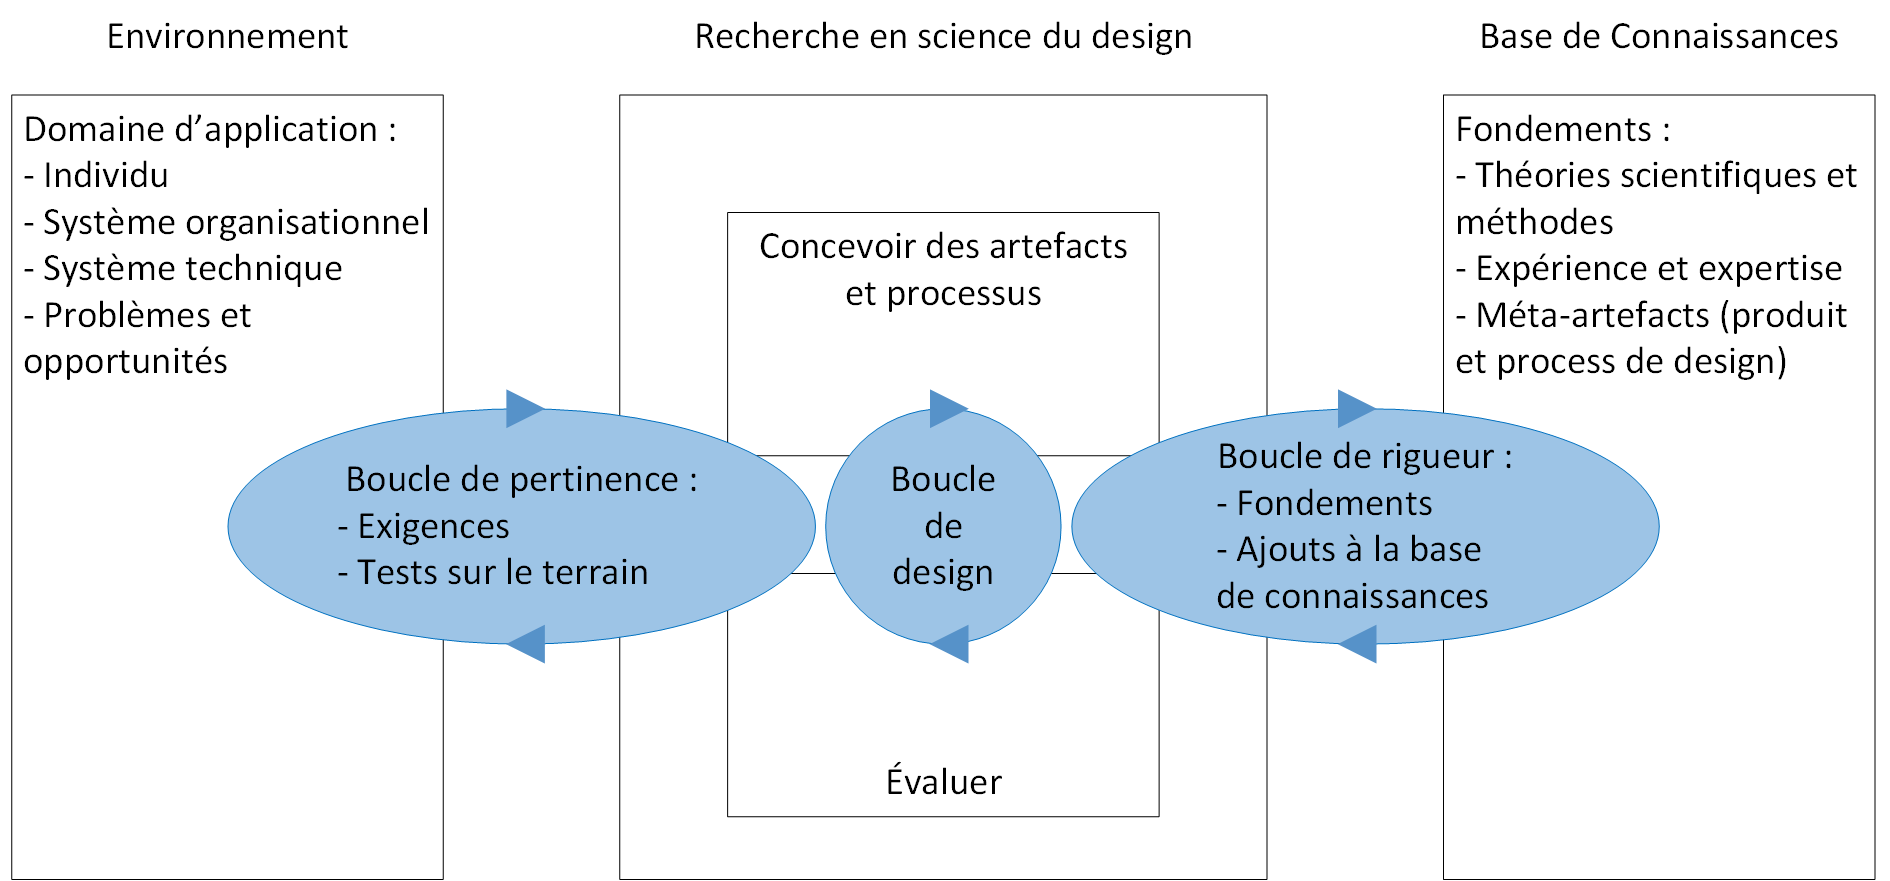
\includegraphics[scale=0.78]{1-Introduction/images/MethodeRecherche/Cycles-Design-Science.png}
}
\caption{Les trois boucles de la science du design présentées dans~\cite{hevner2007three} et \cite{pascal2011approche}}
\label{figure:1-S3-DesignScience-ThreeLoops}
\end{figure}
%\end{figure*} % Figure flottante
% To use it : fig~\ref{label}

\bigskip
%\vspace*{1pt}

Pour répondre à notre question de recherche, nous avons effectué une méthodologie de recherche s'inspirant particulièrement de la science du design.
Tout d'abord, nous avons réalisé une étude du domaine des processus à forte intensité des connaissances et l'avons publié dans un article~\cite{boissier2019challenges}.
Celle-ci a permis de mettre en évidence six défis récurrents dans le domaine des processus à forte intensité de connaissances en étudiant les différents fondements théoriques et réponses actuellement apportées par la recherche.
Cette étude a donc contribué aux boucles de pertinence et de rigueur en construisant un premier cadre.
Afin d'évaluer les résultats d'une contribution pouvant relever certains des défis présentés, nous avons choisi un domaine particulièrement adapté à la manipulation de connaissances et rencontrant actuellement des difficultés suite à la crise du COVID-19 : l'enseignement supérieur et la recherche.
Notre premier objectif a été de proposer une méthode permettant d'aider à construire le cours le plus pertinent possible pour un sujet donné en s'appuyant sur la réutilisation de fragments de processus.
Notre stratégie de validation pour la méthode CREA consiste à la réalisation et l'analyse de cinq scénarios de création de cours ainsi qu'un retour d'expérience basé sur des entretiens.

\bigskip
%\vspace*{1pt}

Un premier scénario servant de cas de référence a été réalisé afin d'établir une première itération de la boucle de design et vérifier les critères attendus pour les domaines de recherche et d'application.
Ce premier scénario vise à rassembler plusieurs supports de cours traitant d'un même sujet, afin de pouvoir en extraire des fragments réutilisables (des notions à présenter à chaque séance de cours).
La boucle de design pouvant fonctionner seule, ce premier scénario nous a permis de fixer certains paramètres au sein de la méthode construite.
Ces paramètres sont présentés au fur et à mesure dans le chapitre~\ref{chapter:CREA}.
De plus, plusieurs directions ont été testées et abandonnées étant donné la faible qualité des résultats apportés.

Nous avons ensuite étendu nos objectifs en ajoutant une détection de la pertinence des supports de cours par rapport à un sujet donné.
Un deuxième scénario a donc été construit en insérant parmi les données d'entrée un document traitant d'un sujet un peu plus éloigné, mais pas complètement hors sujet.
En comparaison du premier scénario, celui-ci doit mettre en évidence que le document supplémentaire est moins pertinent que les autres, et donc qu'il n'est pas conforme.

Un troisième scénario a permis d'étudier l'impact de l'augmentation du nombre de documents sur les métriques de sorties et les clusters générés.
Deux fois plus de documents ont été insérés en entrée pour observer les effets.
Ces trois premiers cas ont surtout permis d'effectuer une validation structurelle de la méthode CREA que nous avons construite, tout en s'assurant de l'absence de problèmes fonctionnels sur le fond.

Un quatrième scénario a permis d'étudier la correction du bruit sur un support et les conséquences sur le graphe d'impact mutuel au fur et à mesure.
Certains documents précédemment utilisés ont été utilisés et l'un d'entre eux a été \textit{corrigé} en lui retirant des sections hors sujet.

Un cinquième scénario a permis d'étudier l'impact de la langue sur les clusters finaux et de la nature des documents sur leur pertinence, tout en s'assurant que la méthode n'a pas été spécialisée sur le cas de référence et ses dérivés.
Plusieurs documents de nature diversifiée en anglais (supports de cours, d'articles de recherche, et de pages web) ont été insérés en entrée.



%%%%%

Enfin, deux questionnaires ont été réalisés sur le cas de référence en interrogeant des experts du sujet traité pour s'assurer que les résultats sont exploitables par des utilisateurs.
Nous présentons dans cette thèse le résultat des multiples itérations de ces trois boucles et les cinq scénarios qui ont permis cela.

\bigskip

Cette méthodologie de recherche manipule elle-même de nombreuses connaissances et réutilise des contributions passées, ou s'en inspire grandement pour avancer plus loin.
Comme tout processus de recherche, il s'agit bien d'un processus à forte intensité de connaissances qui contribue à répondre à un problème de processus à forte intensité de connaissances (condition nécessaire).
La contribution proposée dépendant elle aussi des connaissances implicites de l'utilisateur, ainsi que des connaissances intégrées aux documents et aux bases de connaissances utilisées comme nous l'avons présenté dans les chapitres précédents, il n'y a donc pas de contradiction théorique.




%%%%%%%%%%%%%%%%%%%%%%%%%%%%%%%%%%%%%%%%%%%%
\clearpage % Clean for pictures and tables %
\newpage   % Clean for pictures and tables %
%%%%%%%%%%%%%%%%%%%%%%%%%%%%%%%%%%%%%%%%%%%%

%%%%%%%%%%%%%%%%%%%%%%%%%%%%%%%%%%%%%%%%%%%%%%%%%%%%%%%%%
%%%%%%%%%%%%%%%%%%%%%%%%%%%%%%%%%%%%%%%%%%%%%%%%%%%%%%%%%
%%%%%%%%%%%%%%%%%%%%%%%%%%%%%%%%%%%%%%%%%%%%%%%%%%%%%%%%%
%%%%%%%%%%%%%%%%%%%%%%%%%%%%%%%%%%%%%%%%%%%%%%%%%%%%%%%%%
%%%%%%%%%%%%%%%%%%%%%%%%%%%%%%%%%%%%%%%%%%%%%%%%%%%%%%%%%
%%%%%%%%%%%%%%%%%%%%%%%%%%%%%%%%%%%%%%%%%%%%%%%%%%%%%%%%%

\section{Protocole d'évaluation}
\label{section:Evaluation:ProtocoleEvaluation}


\subsection{Scénarios d'évaluation}
\label{subsection:Evaluation:ProtocoleEvaluation:ScenariosEvaluation}

Cinq scénarios ont été préparés pour pouvoir valider la méthode CREA dans plusieurs situations.
Ces scénarios visent à construire un cours en 8 séances, donc générer 8 clusters.
\begin{itemize}
\item Scénario n°1 (cas référence) : Ce scénario de référence doit pouvoir fournir des clusters de termes pertinents pour un cours de développement web en PHP.
Les clusters de termes générés doivent au moins aider un enseignant à parler des bases du développement du web avec HTML, PHP, et un peu de base de données avec MySQL.
9 supports de cours de PHP sont utilisés, 6 sont au format diapositives et 3 au format texte long.
Tous les documents fournis en entrée sont pertinents, bien qu'ils aient leurs spécificités.
Ceux-ci sont détaillés dans les paragraphes suivants afin de mieux comprendre leurs spécificités et ce qui est attendu dans le graphe d'impact mutuel.
Nous avons également réalisé une étude comparative depuis notre propre point de vue expert sur ce cas de référence.
Enfin, nous avons demandé à 5 informaticiens de construire 8 clusters à partir des termes retenus par la stratégie haute et $ \beta = 1.00 $ pour pouvoir les comparer à ceux produits par la méthode CREA.
Nous leurs avons ensuite demandé de donner leur avis sur les clusters générés par la méthode CREA.
Ainsi, ce scénario contribue à répondre aux hypothèses H1, H2, H3, H4a-b, H5, H6a-b-c, et H8a-b-c en faisant l'extraction des termes d'un premier corpus documentaire traitant d'un même sujet, puis en produisant un premier graphe d'impact mutuel et des clusters.
Ces données seront comparées à celles produites dans les autres scénarios afin de valider ou invalider les hypothèses. \\

\item Scénario n°2 : Ce scénario vise à vérifier la résistance au bruit en insérant un cours sur un sujet éloigné dans le corpus initial.
Les 9 supports de cours de PHP du scénario n°1 sont utilisés, et sont complétés d'un cours de Java au format texte long.
Le document Java traitant de développement, il sera suffisamment proche des cours de PHP pour avoir quelques liens sémantiques, mais le c\oe{}ur du sujet n'étant pas le développement web, ces liens sémantiques seront limités et il devrait apparaitre comme éloigné des autres documents.
Ce scénario se limite à la génération du graphe d'impact mutuel pour permettre à un enseignant de constater qu'un des documents insérés est trop peu pertinent par rapport aux autres, et qu'il faudrait donc le retirer.
Ce deuxième scénario contribue à répondre aux hypothèses H1, H2, H3, H7b, et H8a-b-c en faisant l'extraction des termes d'un deuxième corpus documentaire dont un document est incorrect, puis en produisant un second graphe d'impact mutuel devant faire apparaître une incohérence. \\

\item Scénario n°3 : Ce scénario vise à vérifier la robustesse de la méthode en doublant le nombre de documents par rapport au corpus initial.
18 supports de cours de PHP sont donc utilisés.
9 proviennent du scénario n°1 (6 au format diapositives et 3 au format texte long), et 9 autres sont ajoutés (5 au format diapositives et 4 au format texte long).
Ce troisième scénario contribue à répondre aux hypothèses H1, H2, H3, H4a-b, H5, H6a-b-c, et H8a-b-c en faisant l'extraction des termes d'un troisième corpus documentaire traitant d'un même sujet mais avec beaucoup plus de documents, puis en produisant un troisième graphe d'impact mutuel et des clusters. \\

\item Scénario n°4 : Ce scénario vise à vérifier que la méthode est fonctionnellement correcte en s'assurant que l'amélioration des documents en entrée produit un graphe d'impact mutuel reflétant ces améliorations.
7 supports de cours de PHP sont utilisés parmi les 18 du scénario n°3, en particulier, nous ne sélectionnons que ceux au format texte long.
L'un de ces supports étant considéré comme assez peu cohérent par rapport aux autres, nous étudions succinctement ses différences pour pouvoir le \textit{corriger} deux fois de suite en supprimant des sections hors sujet.
Afin de s'assurer de la validité des corrections, et de leurs conséquences, chaque test est également reproduit une deuxième fois en insérant le support de cours Java parmi les données d'entrée.
Ce quatrième scénario contribue à répondre aux hypothèses H1, H3, H7b, et H8a-b-c en étudiant l'évolution du graphe d'impact mutuel suite aux modifications dans le contenu des documents.

\item Scénario n°5 : Ce scénario a trois objectifs distincts.
Il vise tout d'abord à s'assurer que la méthode n'a pas été construite pour favoriser la détection de cours PHP, étant donné que le cas de référence a été utilisé pour fixer les paramètres tout au long des travaux de cette thèse.
Le second objectif est de valider que la partie traitement automatique du langage supporte d'autres langues, en particulier l'anglais.
Le troisième objectif est de confirmer que les documents pouvant être analysés ne se limitent pas à des supports de cours, mais peuvent être étendus à d'autres formats (page web, articles de recherche, livres, ...).
Nous avons donc testé la méthode CREA sur 13 documents en anglais traitant des Statecharts~\cite{harel1987statecharts}.
Afin de gérer l'anglais, les configurations de TreeTagger et BabelFy ont été adaptées.
Ce cinquième scénario contribue à répondre aux hypothèses H1, H2, H3, H4a-b, H5, H6a-b-c, H7a-c, et H8a-b-c en faisant l'extraction des termes d'un quatrième corpus documentaire beaucoup plus hétérogène traitant d'un sujet différent des précédents, puis en produisant un cinquième graphe d'impact mutuel et des clusters. \\

\end{itemize}

\bigskip


\begin{table}[htb!]
\centering
\centerline{  % FORCE FIGURE OUTSIDE THE MARGIN !!! BUT STILL CENTERING !!!
\begin{tabular}{ c   c   c   c  l  c  c  c  l  c  l  c  c  c  l  c  c  c  l  c  c  c  l  c }
\specialrule{.1em}{.05em}{.05em}
\multirow{2}{*}{} & \multirow{2}{*}{H1} & \multirow{2}{*}{H2} & \multirow{2}{*}{H3} & & \multicolumn{3}{c}{H4} & & \multirow{2}{*}{H5} & & \multicolumn{3}{c}{H6} & & \multicolumn{3}{c}{H7} & & \multicolumn{3}{c}{H8} & & \multirow{2}{*}{H9} \\
\cline{6-8} \cline{12-14} \cline{16-18} \cline{20-22}
                  &                     &                     &                     & &     a & b & c        & &                    &           & a & b & c        & &      a & b & c         & &      a & b & c        & &  \\

\specialrule{.1em}{.05em}{.05em}
%  & H1 & H2 & H3 & H4a & H4b & H4c &
% H5 & H6a & H6b & H6c & H7a & H7b & H7c &
% H8a & H8b & H8c & H9
%
% S1 : H1, H2, H3, H4a-b, H5, H6a-b-c, H8a-b-c
S1 & \textbullet & \textbullet & \textbullet & &  \textbullet & \textbullet & &  &
 \textbullet & &  \textbullet & \textbullet & \textbullet & &  & & &  &
 \textbullet & \textbullet & \textbullet & & \\
\hline
% S2 : H1, H2, H3, H7b, H8a-b-c
S2 & \textbullet & \textbullet & \textbullet & &  & & &  &
 & &   & &  & &  & \textbullet & &  &
 \textbullet & \textbullet & \textbullet & & \\
\hline
% H1, H2, H3, H4a-b, H5, H6a-b-c, H8a-b-c
S3 & \textbullet & \textbullet & \textbullet & &  \textbullet & \textbullet &  & &
 \textbullet & &  \textbullet & \textbullet & \textbullet & &  & & &  &
 \textbullet & \textbullet & \textbullet & & \\
\hline
% H1, H3, H7b, H8a-b-c
S4 & \textbullet & & \textbullet & &  & & &  &
 & &  & &  & &  & \textbullet & &  &
 \textbullet & \textbullet & \textbullet & & \\
\hline
% H1, H2, H3, H4a-b, H5, H6a-b-c, H7a-c, H8a-b-c
S5 & \textbullet & \textbullet & \textbullet & &  \textbullet & \textbullet &  & &
 \textbullet & &  \textbullet & \textbullet & \textbullet & &  \textbullet & & \textbullet &  &
 \textbullet & \textbullet & \textbullet & & \\
\specialrule{.1em}{.05em}{.05em}
\end{tabular}
}
\caption{Scénarios et hypothèses visées}
\label{table:4-Scenarios-Hypotheses}
\end{table}




\subsection{Validations structurelles, fonctionnelles, et par retour d'expérience}
\label{subsection:Evaluation:ProtocoleEvaluation:ValidationsStructurellesFonctionnellesREX}

Afin d'évaluer la méthode CREA, nous avons effectué plusieurs validations structurelles et fonctionnelles.
Nous nous assurons ainsi que chaque composant fonctionne, et que l'ensemble de la méthode CREA génère des résultats utiles pour un enseignant.


\subsubsection{Validations structurelles}
\label{subsubsection:Evaluation:ProtocoleEvaluation:ValidationsStructurellesFonctionnellesREX:Structurelle}

La validation structurelle du point de vue design science est décrite ainsi dans~\cite{hevner2004design} : \og \textit{Perform coverage testing of some metric (e.g., execution paths) in the artifact implementation} \fg , c'est-à-dire qu'elle vérifie certaines métriques dans l'artefact implémenté.
Elle est plus spécifiquement comparée au fonctionnement \og \textit{White Box} \fg dans lequel les composants d'un artefact sont connus avec précision, et sont testés un à un.

\bigskip

Pour effectuer la validation structurelle, nous comparons plusieurs valeurs par rapport aux documents d'entrée :
\begin{itemize}
\item Nous comptons le nombre de \textit{mots} (suite de caractères séparés par des espaces, de la ponctuation, ou des retours à la ligne) et de \textit{termes} (ensemble de mots formant un concept ou une entité nommée dans le réseau sémantique BabelNet lors de l'étape de désambiguïsation (PI.3)) dans chaque document, et nous les comparons au nombre de mots et termes conservés suite  aux étape de nettoyage des textes (PI.2) et  de filtrage des termes (PI.4).
Les pourcentages de mots et de termes conservés sont également indiqués.
Cette métrique permet de comparer les documents entre eux en cas de disproportions dans les quantités de mots ou de termes, et d'observer les conséquences sur les résultats intermédiaires et finaux.\\

\item Nous comptons le nombre de \textit{termes uniques} (entités nommées et concepts retrouvés dans le réseau sémantique BabelNet lors de l'étape de désambiguïsation (PI.3), sans prendre en compte les occurrences) retenus et exclus dans chaque document, et nous le comparons au nombre de termes uniques retenus et exclus suite à l'étape de filtrage des termes (PI.4).
Les pourcentages de termes uniques retenus et exclus, et le nombre de termes communs aux deux listes sont également indiqués.
Cette métrique permet de comparer les documents entre eux en cas de disproportions dans les quantités de termes uniques, et d'observer les conséquences sur les résultats intermédiaires et finaux.
Les termes communs servent également à mesurer le nombre de termes dont le contexte détecté par BabelFy ne correspond pas à celui qui serait attendu ou dont la désambiguïsation n'est pas sûre.\\

\item Nous comptons la quantité de termes uniques retenus pour les quatre stratégies de binarisation (directe, moyenne, haute, basse) appliquées avec cinq valeurs de $ \beta $ allant de $ 0.00 $ à $ 1.00 $ par pas de $ 0.25 $.
Cette métrique permet de vérifier la quantité de termes uniques retenus par les stratégies, et estimer la valeur de $ \beta $ la plus adaptée pour sélectionner les termes les plus importants/retirer les termes pouvant provoquer du bruit dans les traitements suivants.
Elle vise également à confirmer que les stratégies directe et haute conservent respectivement le plus de termes et une quantité limitée mais suffisante de termes pour les traitements suivants.\\

\item Nous comptons la quantité et les proportions de \og 0 \fg et de \og 1 \fg dans les matrices générées par les quatre stratégies de binarisation et les cinq valeurs de $ \beta $.
Cette métrique permet de s'assurer que les treillis générés ne seront ni trop vides (beaucoup trop de \og 0 \fg forment quelques concepts formels aux extrémités du treillis uniquement), ni trop pleins (beaucoup trop de \og 1 \fg forment toutes les combinaisons possibles de documents et de termes), mais feront suffisamment de liens entre les termes et les documents pour que des concepts formels intéressants soient formés (c'est-à-dire qu'il existe des concepts formels mélangeant plusieurs documents \textit{et} plusieurs termes, sans produire toutes les combinaisons possibles).\\

\item Nous analysons les clusters générés avec la stratégie haute afin de confirmer que le choix du $ \beta $ à $ 1.00 $ est adapté.
Les clusters générés sont comparés pour connaître le $ \beta $ générant les meilleurs clusters (c'est-à-dire ceux contenant le moins de bruit, et dont l'organisation est la plus correcte pour un expert).
Cette analyse est également réalisée avec la validation fonctionnelle étant donné qu'elle concerne la sortie finale.
\end{itemize}


\subsubsection{Validations fonctionnelles}
\label{subsubsection:Evaluation:ProtocoleEvaluation:ValidationsStructurellesFonctionnellesREX:Fonctionnelle}

La validation fonctionnelle du point de vue design science est décrite ainsi dans~\cite{hevner2004design} : \og \textit{Execute artifact interfaces to discover failures and identify defects} \fg , c'est-à-dire qu'elle vérifie si l'artefact présente des défaillances à l'usage.
Elle est plus spécifiquement comparée au fonctionnement \og \textit{Black Box} \fg dans lequel les composants d'un artefact sont inconnus, et seules les entrées et sorties peuvent être contrôlées.

\bigskip

Pour effectuer la validation fonctionnelle, nous analysons cette fois les données produites en sortie de la méthode pour chaque cas :
\begin{itemize}
\item Nous analysons le graphe d'impact mutuel formé grâce aux métriques du treillis avec la stratégie directe lors de l'étape calcul des métriques du treillis (PII.1.e) afin d'évaluer si la méthode détecte correctement quels documents portent sur le même sujet, et lesquels en sont éloignés.
La validation étant visuelle, nous observons donc quels documents sont suffisamment rapprochés pour former un groupe au centre du graphique, et quels documents sont au contraire éloignés du centre.\\

\item Nous analysons les clusters générés avec la stratégie haute afin de confirmer que la méthode fonctionne et produit des clusters pertinents pour la réutilisation.
Cette validation étant purement qualitative, nous nous sommes permis d'évaluer avec notre propre expertise les résultats.
Pour confirmer la pertinence des clusters, nous avons également demandé à des informaticiens leurs avis sur un cas servant de référence.
\end{itemize}



%\bigskip

\subsubsection{Validation par retour d'expérience}
\label{subsubsection:Evaluation:ProtocoleEvaluation:ValidationsStructurellesFonctionnellesREX:REX}


Nous avons également réalisé des entretiens en demandant un avis extérieur sur la qualité des clusters générés par la méthode CREA.
Pour cela, 5 informaticiens ont été interrogés avec deux questionnaires successifs (le deuxième n'étant envoyé qu'une fois le premier récupéré) à propos des résultats du scénario n°1 (les 9 supports de cours de développement web en PHP).
2 informaticiens sont novices en PHP (faible expérience en développement web avec PHP ou en administration d'un serveur web utilisant PHP).
3 informaticiens sont experts en PHP (nombreuses expériences en développement web, déploiement d'applications, et administration d'applications utilisant PHP).
Parmi les 3 experts en PHP, 2 ont une expérience dans l'enseignement de l'informatique et en particulier des langages de programmation.
L'objectif de diviser en deux questionnaires séparés est de récupérer tout d'abord l'avis individuel de chacun (en utilisant leurs connaissances tacites) sur l'organisation du cours idéal avec les termes uniques obtenus, avant de demander un avis critique sur les résultats de la méthode CREA.

\bigskip

Afin de connaître plusieurs dispositions possibles du point de vue humain, le premier questionnaire demande d'organiser les 60 termes issus du scénario n°1 en 8 clusters.
Les consignes suivantes ont été envoyées avec une feuille excel contenant l'ensemble des termes :
\begin{verbatim}
ORGANISER LES 60 TERMES EN 8 SEANCES DE COURS
				(voir onglet/feuille "Clusters" tout en bas)
CONTRAINTES :
 - au moins 1 terme par séance (une séance est représentée par un cluster)
 - chaque terme doit être au plus ET au moins dans une séance
\end{verbatim}

\bigskip

Le deuxième questionnaire présente tout d'abord les clusters du cas de référence avant de poser 4 questions.
Les 2 premières nous intéressent particulièrement pour cette expérience, les 2 autres servant pour des travaux ultérieurs sur l'axe temporel (voir sous-section~\ref{subsection:Conclusion:PerspectivesAmeliorations:AnalyseTemporelle} en conclusion).
Les questions sont posées comme suit :
\begin{enumerate}
\item Notez cette proposition de regroupements :
	\begin{itemize}
	\item[] (0) Les regroupements n'ont aucun sens pour un cours de PHP
		[aucun terme ne va avec un autre dans un même cluster pour faire un cours de PHP]

	\item[] (1) Seuls quelques regroupements ont un peu de logique
		[beaucoup de clusters contiennent des termes qui n'ont aucun lien entre eux pour faire un cours de PHP]
	\item[] (2) Les termes sont vaguement liés, ce serait très difficile d'en faire un cours de PHP
		[les clusters nécessitent tous au moins plusieurs modifications pour être utilisables pour faire un cours de PHP]
	\item[] (3) Les termes sont plutôt liés, mais il y a beaucoup trop de bruit pour pouvoir facilement construire un cours PHP
		[quelques clusters ont besoin d'être profondément modifiés pour faire un cours de PHP]

	\item[] (4) Les termes sont quasiment tous liés, il y a un peu de bruit, mais il est possible de construire un cours de PHP
		[les clusters sont majoritairement bons, quelques-uns ont besoin de quelques modifications pour faire un cours de PHP]

	\item[] (5) Les termes sont correctement liés, un cours peut directement en être produit
		[aucune modification n'est requise : un cours de PHP peut directement être produit]
	\end{itemize}

\item Expliquez votre choix :

\item À quel moment placeriez-vous chacun des clusters pour faire un cours de PHP ?
	\begin{itemize}
	\item[] Début :
	\item[] Milieu :
	\item[] Fin :
	\end{itemize}

\item Dans quel ordre très précis placeriez-vous chacun des clusters pour faire un cours ?
	(si vous avez un doute sur certain(s), indiquez si vous avez un doute entre plusieurs endroits OU si vous n'arrivez absolument pas à le placer)
	\begin{itemize}
	\item[] Ordre :
	\item[] Doute 1 : (hésitation entre plusieurs moments pour le placer)
	\item[]	Doute 2 : (aucune idée du moment où le placer)
	\end{itemize}
\end{enumerate}


\bigskip

Les réponses au premier questionnaire sont comparées avec l'indice de Rand~\cite{rand1971objective} et l'indice de Rand ajusté~\cite{hubert1985comparing} afin de déterminer les différences entre chacune des réponses.
Ces deux indices permettent de comparer deux partitions, c'est-à-dire comparer dans deux cas la façon dont des éléments ont été regroupés dans des clusters.

L'indice de Rand~\cite{rand1971objective} produit une mesure de similarité en comparant des paires de points entre chacune des deux partitions.
Cette mesure produit un résultat allant de $ 1 $ (les deux partitions ont strictement les mêmes clusters contenant exactement les mêmes points) à $ 0 $ (les deux partitions n'ont strictement aucune paire de points regroupée dans les mêmes clusters, par exemple comme expliqué dans~\cite{rand1971objective} : une première partition a tous ses points regroupés dans un unique cluster, et une deuxième partition a autant de clusters qu'il y a de points).
Pour calculer l'indice de Rand, on s'intéresse particulièrement à quatre types de paires de points dans chacune des deux partitions testées~\cite{hubert1985comparing}\cite{steinley2004properties} :
\begin{itemize}
\item \textit{a} : les paires de points appartenant dans les deux cas aux mêmes clusters (exemple figure~\ref{figure:4-RandIndex} : \textit{Terme 2} et \textit{Terme 4} sont ensemble dans les deux cas)
\item \textit{b} : les paires de points appartenant à des classes différentes dans le premier cas, et à la même classe dans le deuxième cas (exemple figure~\ref{figure:4-RandIndex} : \textit{Terme 1} et \textit{Terme 3} sont dans les clusters \textit{I} et \textit{II} dans le cas n°1, puis dans le cluster \textit{A} dans le cas n°2)
\item \textit{c} : les paires de points appartenant à la même classe dans le premier cas, et à des classes différentes dans le deuxième cas (exemple figure~\ref{figure:4-RandIndex} : \textit{Terme 1} et \textit{Terme 2} sont dans le cluster \textit{I} dans le cas n°1, puis dans les clusters \textit{A} et \textit{B} dans le cas n°2)
\item \textit{d} : les paires de points appartenant à des classes différentes dans les deux cas (exemple figure~\ref{figure:4-RandIndex} : \textit{Terme 1} et \textit{Terme 6} sont dans des clusters différents dans les deux cas)
\end{itemize}
Un autre point de vue permet de considérer les types de paires \textit{a} et \textit{d} comme étant en \textit{accord} (les paires de points sont ensemble dans les deux cas, ou séparées dans les deux cas), et les types de paires \textit{b} et \textit{c} comme étant en \textit{désaccord} (les paires de points sont ensemble dans un cas, et séparées dans l'autre cas).
L'indice de Rand se calcule précisément par le rapport décrit dans l'équation~\eqref{equation:4-RandIndex}, où \textit{a}, \textit{b}, \textit{c}, \textit{d} correspondent aux nombres de paires de chaque type.
On notera que l'indice de Rand est symétrique.

\begin{equation}
RI(\text{\textit{Cas n°1}}, \text{\textit{Cas n°2}}) = \frac{a + d}{a + b + c + d}
\label{equation:4-RandIndex}
\end{equation}


\bigskip


\begin{figure}[ht]
\centering
\centerline{  % FORCE FIGURE OUTSIDE THE MARGIN !!! BUT STILL CENTERING !!!
% scale = 0.7    0.68 (sans enumerate)
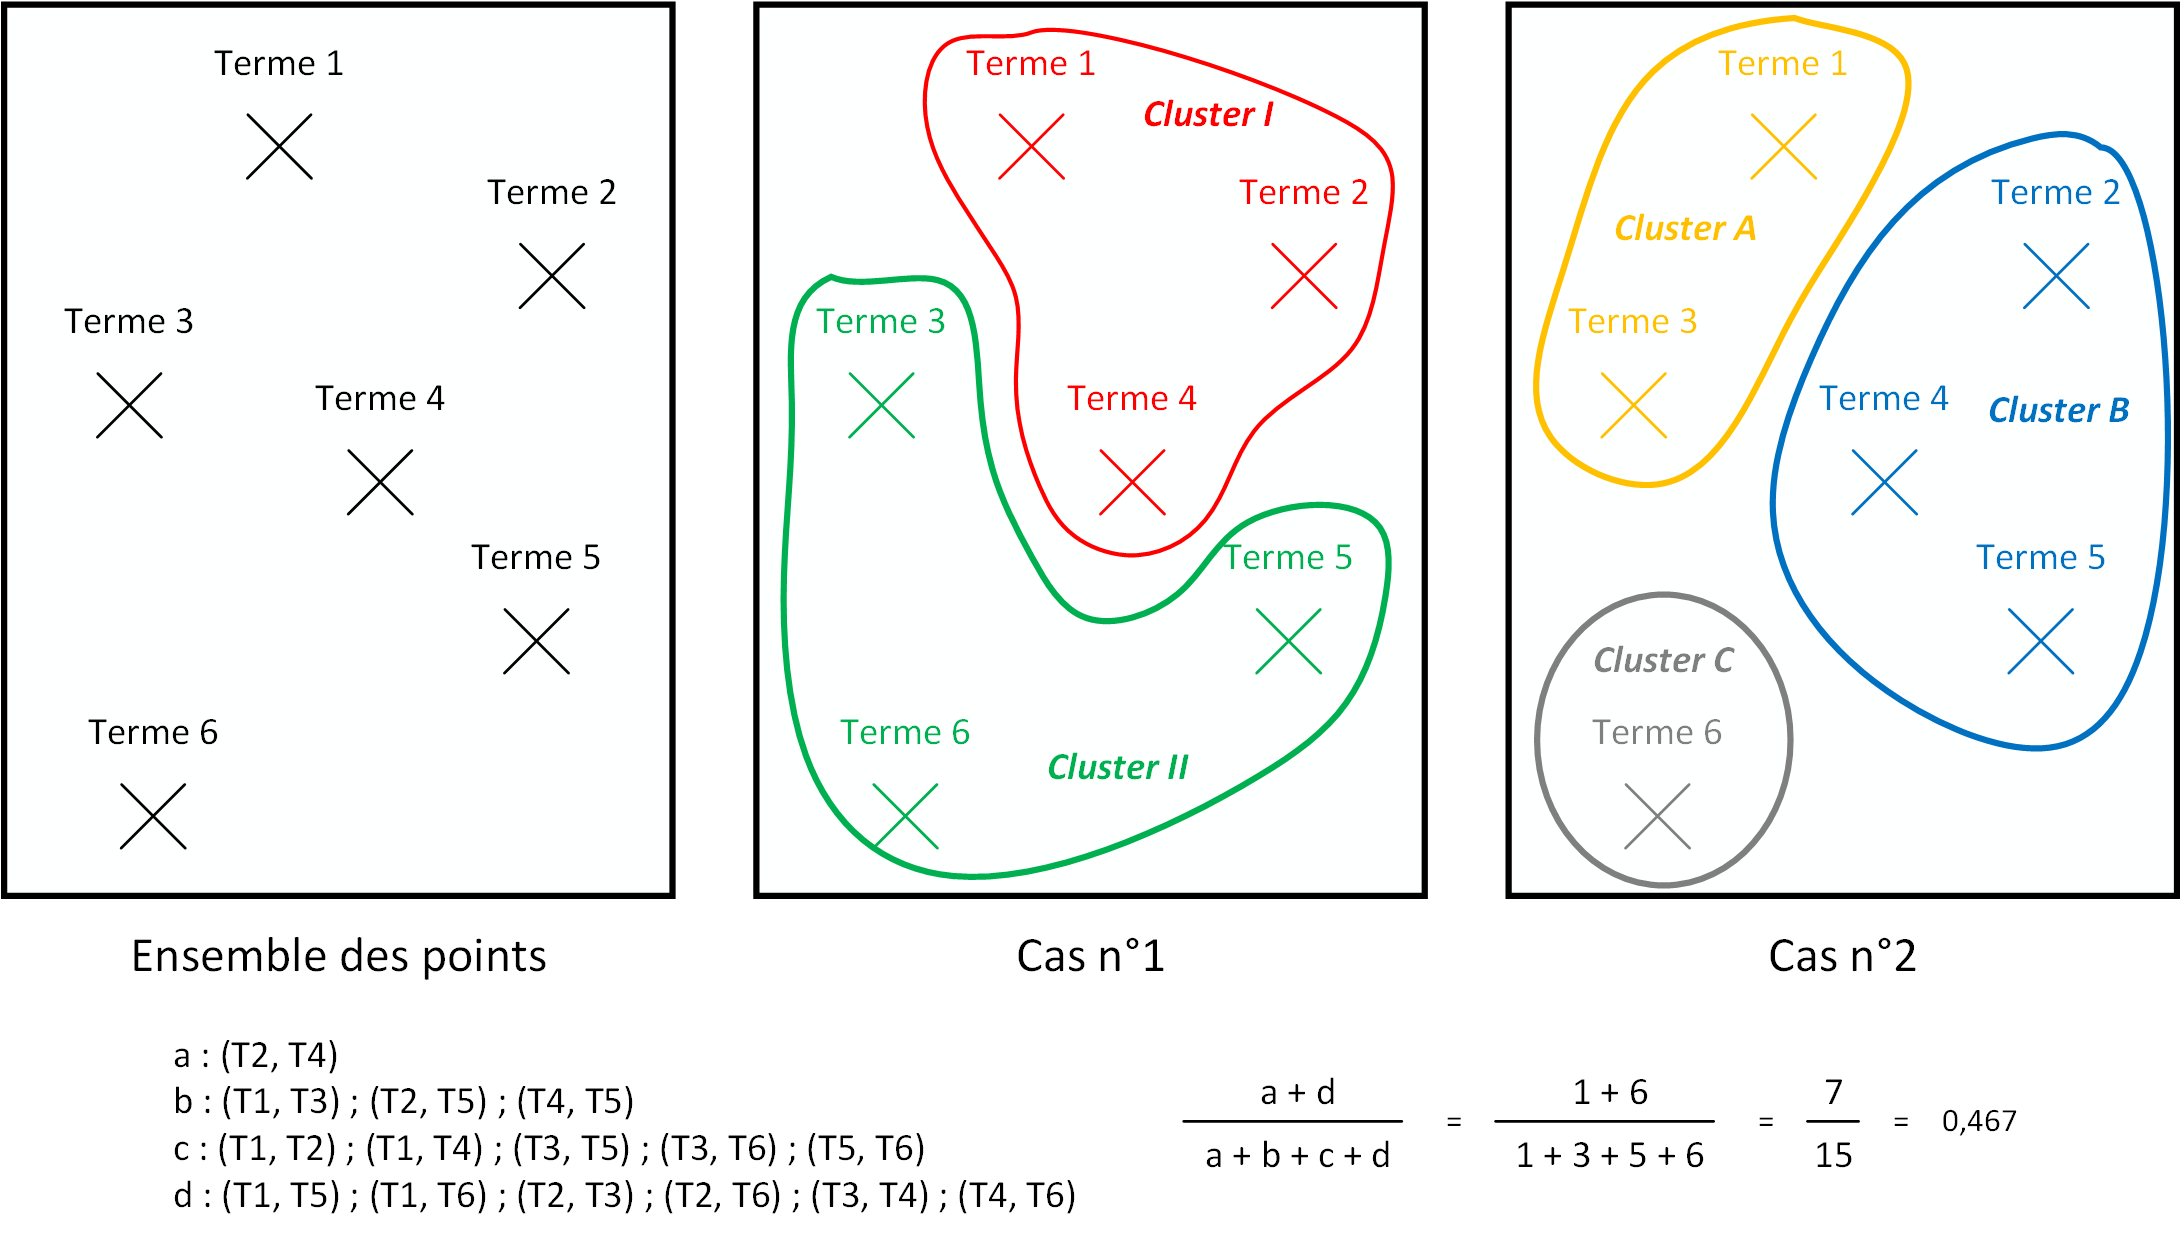
\includegraphics[scale=0.55]{4-Experiences/images/cas-5/RandIndex-formula.png}
}
\caption{Exemple de points, de deux partitions différentes, et du calcul de l'index de Rand}
\label{figure:4-RandIndex}
\end{figure}

\bigskip

L'indice de Rand ajusté~\cite{hubert1985comparing} vise à prendre en compte le fait que certaines paires de points considérées comme en accord ne le sont que par hasard.
Le point de vue utilisé par cet indice est légèrement différent : il teste la possibilité que les deux partitions aient été construites au hasard, tout en s'appuyant sur la considération qu'une des partitions est considérée comme correcte (\og \textit{ground truth} \fg) et que l'autre est testée pour connaître sa similarité.
L'indice de Rand ajusté corrige également certains défauts de l'indice de Rand original, notamment le fait que la valeur générée s'approche rapidement de $ 1 $ lorsque le nombre de clusters augmente~\cite{quere:tel-00950514}.
Concernant l'interprétation, un indice de Rand ajusté proche de $ 1 $ implique que les deux partitions sont identiques, et un indice proche de $ 0 $ indique que les partitions ont été générées aléatoirement~\cite{quere:tel-00950514} (les valeurs peuvent également être négatives).
Nous ne détaillerons pas la construction de l'indice de Rand ajusté dans cette thèse, mais il est intéressant de noter que celui-ci est également symétrique.



%%%%%%%%%%%%%%%%%%%%%%%%%%%%%%%%%%%%%%%%%%%%
\clearpage % Clean for pictures and tables %
\newpage   % Clean for pictures and tables %
%%%%%%%%%%%%%%%%%%%%%%%%%%%%%%%%%%%%%%%%%%%%

%%%%%%%%%%%%%%%%%%%%%%%%%%%%%%%%%%%%%%%%%%%%%%%%%%%%%%%%%
%%%%%%%%%%%%%%%%%%%%%%%%%%%%%%%%%%%%%%%%%%%%%%%%%%%%%%%%%
%%%%%%%%%%%%%%%%%%%%%%%%%%%%%%%%%%%%%%%%%%%%%%%%%%%%%%%%%
%%%%%%%%%%%%%%%%%%%%%%%%%%%%%%%%%%%%%%%%%%%%%%%%%%%%%%%%%
%%%%%%%%%%%%%%%%%%%%%%%%%%%%%%%%%%%%%%%%%%%%%%%%%%%%%%%%%

\section{Déroulement des expérimentations}
\label{section:Evaluation:DeroulementExperimentations}

Dans cette section, nous présentons tout d'abord les 9 supports de cours du scénario 1 plus en détails, étant donné que ce scénario sert de référence pour plusieurs expériences.
Nous disposons ensuite succinctement l'ensemble des supports utilisés lors des différentes validations.
Les résultats bruts de chaque étape de la méthode CREA, ainsi que les résultats finaux (graphe d'impact mutuel, et clusters de termes), sont finalement exposés.


\subsection{Présentation détaillée des documents du cas de référence}
\label{subsection:Evaluation:DeroulementExperimentations:PresentationDocumentsCasRef}


%\paragraph{C1 (E.Coquery) Cours HTML/PHP :}

\begin{table}[ht!]
\centerline{
\begin{tabular}{| m{5cm} m{10cm} |}
\hline
Document :						& \textbf{C1} \\
Titre : 						& \textit{Cours HTML/PHP} \\
Auteur : 						& E.Coquery \\
Type de document : 				& diapositives \\
Année : 						& 2008\\
Nb pages/diapositives : 		& 46 \\
En-têtes et/ou en-pieds : 		& Oui \\
Mots clés : 					& HTML, liens hypertexte, formulaires, PHP, opérateurs, tableaux, structure de contrôle, fonctions, GET, POST, MySQL, sessions\\
Niveau du public : 				& Débutant \\
Commentaires :					&  C1 est divisé en 3 sections : les pages webs statiques/dynamiques, HTML, puis PHP.
									Quelques schémas illustrent le cours, mais restent en quantité limité.
									Les diapositives contiennent beaucoup d'exemples de code, mais également les mots clés pour un tel cours.\\
\hline
\end{tabular}
}
\end{table}



%\paragraph{C2 (T.Lecroq) PHP :}

\begin{table}[ht!]
\centerline{
\begin{tabular}{| m{5cm} m{10cm} |}
\hline
Document :						& \textbf{C2} \\
Titre : 						& \textit{PHP} \\
Auteur : 						& T.Lecroq \\
Type de document : 				& diapositives \\
Année : 						& 2009 \\
Nb pages/diapositives : 		& 64 \\
En-têtes et/ou en-pieds : 		& Oui \\
Mots clés : 					& XHTML, formulaires, PHP, tableaux, instructions de contrôle, chaînes de caractères, fonctions, transfert de fichiers, lecture, écriture, cookies, sessions, XHTML 2.0, X/HTML 5 \\
Niveau du public : 				& Débutant \\
Commentaires :					& C2 est divisé en 7 sections se concentrant majoritairement sur PHP. \\
\hline
\end{tabular}
}
\end{table}



%\paragraph{C3 (S.Rohaut) Cours PHP - Versions 4.x et 5.x :}

\begin{table}[ht!]
\centerline{
\begin{tabular}{| m{5cm} m{10cm} |}
\hline
Document :						& \textbf{C3} \\
Titre : 						& \textit{Cours PHP - Versions 4.x et 5.x} \\
Auteur : 						& S.Rohaut \\
Type de document : 				& texte \\
Année : 						& 2006 \\
Nb pages/diapositives : 		& 93 \\
En-têtes et/ou en-pieds : 		& Oui \\
Mots clés : 					& PHP, ASP, CGI, HTML, syntaxe, variables, opérateurs, expression, structure de contrôle, fonctions, formulaires, GET, POST, dates, MySQL, PhpMyAdmin, MysqlCC, SQL, types colonnes, types tables, index de tables, fichiers, bases de données, sessions, cookies, images, POO, PHP 4, PHP 5\\
Niveau du public : 				& Moyen \\
Commentaires :					& C3 est divisé en 17 chapitres.
									Le cours introduit surtout les nouveautés de PHP 5 par rapport à PHP 4 (particulièrement la programmation orientée objet). \\
\hline
\end{tabular}
}
\end{table}



%\paragraph{C4 (V.Pagé) Programmation Spécifique : Programmation Web :}

\begin{table}[ht!]
\centerline{
\begin{tabular}{| m{5cm} m{10cm} |}
\hline
Document :						& \textbf{C4} \\
Titre : 						& \textit{Programmation Spécifique : Programmation Web} \\
Auteur : 						& V.Pagé \\
Type de document : 				& diapositives \\
Année : 						& 2007 \\
Nb pages/diapositives : 		& 99 \\
En-têtes et/ou en-pieds : 		& Oui \\
Mots clés : 					& HTML, client web, serveur web, CSS, PHP, fonctionnement, instructions, variables, chaînes de carcatères, tableaux, fonctions, inclusion de fichiers, variables pré-définies, portée des variables, formulaires, cookies, sessions, fichiers, base de données, Postregress, images, GD, sécurité\\
Niveau du public : 				& Débutant \\
Commentaires :					& C4 est divisé en 2 parties : l'une sur HTML, et l'autre sur PHP et MySQL.
									Le cours se termine sur une mention de la gestion d'images avec GD (mais le contenu est absent), et une mention sur la sécurité. \\
\hline
\end{tabular}
}
\end{table}



%\paragraph{C5 (G.Rozsavolgyi) Cours PHP Accéléré :}

\begin{table}[ht!]
\centerline{
\begin{tabular}{| m{5cm} m{10cm} |}
\hline
Document :						& \textbf{C5} \\
Titre : 						& \textit{Cours PHP Accéléré} \\
Auteur : 						& G.Rozsavolgyi \\
Type de document : 				& texte \\
Année : 						& 2018 \\
Nb pages/diapositives : 		& 115 \\
En-têtes et/ou en-pieds : 		& Oui \\
Mots clés : 					& caractéristiques, historique, installation, configuration, HTML, PHP, bases du langage, tableaux, inclusion de fichiers, POO, base de données, SQL, PDO, transactions, connexions persistantes, sessions, cookies, HTTP, XML, MVC, templates, frameworks, Composer, Symfony, Flex, tests, TDD, web services, REST, API, Git\\
Niveau du public : 				& Intermédiaire \\
Commentaires :					& C5 aborde quasiment toutes les notions possibles en une quarantaine de sections.
									Le document contient quelques mentions sur des feuilles de TD. \\
\hline
\end{tabular}
}
\end{table}



%\paragraph{C6 (D.Gonzalez) PHP, une initiation :}

\begin{table}[ht!]
\centerline{
\begin{tabular}{| m{5cm} m{10cm} |}
\hline
Document :						& \textbf{C6} \\
Titre : 						& \textit{PHP, une initiation} \\
Auteur : 						& D.Gonzalez \\
Type de document : 				& texte \\
Année : 						& 2009 \\
Nb pages/diapositives : 		& 160 \\
En-têtes et/ou en-pieds : 		& Non \\
Mots clés : 					& langages informatiques, langages webs, PHP, Javascript, bases du langage, fonctions, formulaires, HTML, chaînes de caractères, tableaux, connecteur, PDO, instructions, SQL, inclusion de fichiers, gestion de l'identification des utilisateurs, sécurité, sessions\\
Niveau du public : 				& Débutant \\
Commentaires :					& C6 est divisé en 4 chapitres : le cours, le cours hors programme, les corrigés des exercices, et des études de cas.
									Le document démarre sur une présentation du document lui-même, puis aborde les notions du cours.
									Le cours contient un peu de bruit au début avec diverses mentions de copyright, licences, et du projet GNU, puis les façons de retrouver le document.
									\textit{Seul le premier chapitre contient le cours}.
									Un mini projet est présenté dans les pages 59 et 60.
									De la page 65 à 93, des corrigés d'exercices sont présents.
									Puis, de la page 93 à 149, des projets sont présentés.\\
\hline
\end{tabular}
}
\end{table}



%\paragraph{C7 (C.Escazut) Le Langage PHP, Ou comment concevoir des sites dynamiques :}

\begin{table}[ht!]
\centerline{
\begin{tabular}{| m{5cm} m{10cm} |}
\hline
Document :						& \textbf{C7} \\
Titre : 						& \textit{Le Langage PHP, Ou comment concevoir des sites dynamiques} \\
Auteur : 						& C.Escazut \\
Type de document : 				& diapositives \\
Année :							& 2017 \\
Nb pages/diapositives :			& 37 \\
En-têtes et/ou en-pieds :		& Oui \\
Mots clés :						& bases du langage, PHP, intégration, HTML, variabes, structures conditionnelles, structures itératives, tableaux, fonctions, formulaires, variables super globales, sessions, cookies\\
Niveau du public :				& Débutant \\
Commentaires :					& C7 est le document le plus court, sa structure se divise en 7 sections.
									Quelques images montrent des exemples de code. \\
\hline
\end{tabular}
}
\end{table}



%\paragraph{C8 (M.Kirsch Pinheiro) Création d'un site Web dynamique PHP :}

\begin{table}[ht!]
\centerline{
\begin{tabular}{| m{5cm} m{10cm} |}
\hline
Document :						& \textbf{C8} \\
Titre : 						& \textit{Création d'un site Web dynamique PHP} \\
Auteur : 						& M.Kirsch Pinheiro \\
Type de document : 				& diapositives \\
Année : 						& 2017 \\
Nb pages/diapositives : 		& 81 \\
En-têtes et/ou en-pieds : 		& Oui \\
Mots clés : 					& bases du langage, PHP, intégration, HTML, interprétation, variable, type, opérateurs, tableaux, POO, classes, objets, constructeurs, formulaires, GET, POST, instructions de contrôle, fonctions, conditions, boucles, importation de fichiers, bases de données, SQL, MySQL, PDO, MySQLi, sessions, cookies\\
Niveau du public : 				& Débutant \\
Commentaires :					& C8 est divisé en 6 sections.
									Le document ayant été construit avec PowerPoint et des cadres se superposant les uns aux autres, les textes extraits automatiquement contiennent parfois des erreurs dans les mots (plusieurs mots sont fusionnés en un).
									Un exercice termine le cours.\\
\hline
\end{tabular}
}
\end{table}



%\paragraph{C9 (L.Dounas) Base de donnée 2: PHP and Mysql :}

\begin{table}[ht!]
\centerline{
\begin{tabular}{| m{5cm} m{10cm} |}
\hline
Document :						& \textbf{C9} \\
Titre : 						& \textit{Base de donnée 2: PHP and Mysql} \\
Auteur : 						& L.Dounas \\
Type de document : 				& diapositives \\
Année : 						& 2018\\
Nb pages/diapositives : 		& 131 \\
En-têtes et/ou en-pieds : 		& \\
Mots clés : 					& SQL, web, PHP, installation, commentaires, types de données, opérateurs, date, constantes, tableaux, conditions, boucles, fonctions, intégration, HTML, chaînes de caractères, formulaires, GET, POST, portée des variables, super-globales, inclusion de fichiers, redirections automatiques, sessions, cookies, POO, calsse, objet, héritage, polymorphisme, constructeur, visibilité des méthodes, static, opérateur ::, abstraction, constantes de classe, final, SGBD, PhpMyAdmin, MySQL, MySQLi, PDO, erreurs, try catch, transactions, ACID, moteurs de stockage\\
Niveau du public : 				& Débutant \\
Commentaires :					& C9 est divisé en 11 sections.
									Plusieurs exercices sont présents au sein du document, ainsi que des références à la fin.\\
\hline
\end{tabular}
}
\end{table}




%%%%%%%%%%%%%%%%%%%%%%%%%%%%%%%%%%%%%%%%%%%%
\clearpage % Clean for pictures and tables %
\newpage   % Clean for pictures and tables %
%%%%%%%%%%%%%%%%%%%%%%%%%%%%%%%%%%%%%%%%%%%%

%%%%%%%%%%%%%%%%%%%%%%%%%%%%%%%%%%%%%%%%%%%%%%%%%%%%%%%%%

\subsection{Présentation succincte des documents}
\label{subsection:Evaluation:DeroulementExperimentations:PresentationDocumentsTousCas}

Comme indiqué dans le protocole d'évaluation en section~\ref{section:Evaluation:ProtocoleEvaluation}, les documents C1 à C9 sont utilisés dans les trois premiers scénarios.
Le document CJA correspond au document Java utilisé dans le scénario n°2.
Le scénario n°3 s'appuie sur les documents C1 à C9 et C11 à C19.
Tous ces documents sont en français.

\bigskip

\hspace{0pt}
\vfill


\begin{table}[htb!]
\centering
\centerline{ %%%%%%%% CENTRER HORS DES MARGES
\begin{tabular}{|c| c | c | c | c | m{6cm} |}
\hline
\textbf{} & \textbf{ID} & \textbf{Format} & \textbf{Nb Pages} & \textbf{Auteur} & \textbf{Titre} \\
\hline
\multirow{9}{*}{S1} & C1 & Diapositives & 46 & E.Coquery & Cours HTML/PHP \\ \cline{2-6}
 & C2 & Diapositives & 64 & T.Lecroq & PHP \\ \cline{2-6}
 & C3 & Texte & 93 & S.Rohaut & Cours PHP - Versions 4.x et 5.x \\ \cline{2-6}
 & C4 & Diapositives & 99 & V.Pagé & Programmation Spécifique : Programmation Web \\ \cline{2-6}
 & C5 & Texte & 115 & G.Rozsavolgyi & Cours PHP Accéléré \\ \cline{2-6}
 & C6 & Texte & 160 & D.Gonzalez & PHP, une initiation \\ \cline{2-6}
 & C7 & Diapositives & 37 & C.Escazut & Le Langage PHP, Ou comment concevoir des sites dynamiques \\ \cline{2-6}
 & C8 & Diapositives & 81 & M.Kirsch Pinheiro & Création d'un site Web dynamique PHP \\ \cline{2-6}
 & C9 & Diapositives & 131 & L.Dounas & Base de donnée 2: PHP and Mysql \\ \hline
\hline
\multirow{1}{*}{S2} & CJA & Texte & 88 & A.Morelle & LE LANGAGE JAVA - Petit mémento de syntaxe \& éléments de programmation \\ \hline
\hline
\multirow{9}{*}{S3} & C11 & Texte & 129 & E.Vandeput & Développer une application avec PHP et MySQL \\ \cline{2-6}
 & C12 & Diapositives & 134 & J.Gaulmin & Programmer en PHP \\ \cline{2-6}
 & C13 & Diapositives & 74 & L.Pouilloux & Projets Web - L3STEP \\ \cline{2-6}
 & C14 & Diapositives & 99 & T.Fressin & Développement web \\ \cline{2-6}
 & C15 & Texte & 113 & D.Hadjadj & Initiation à la programmation de page web en PHP \\ \cline{2-6}
 & C16 & Diapositives & 137 & V.Sans & Programmation Web : PHP \\ \cline{2-6}
 & C17 & Texte & 30 & R.Mokadem & Cours introductif au PHP \\ \cline{2-6}
 & C18 & Diapositives & 82 & V.Ricard & PHP (ET MYSQL) \\ \cline{2-6}
 & C19 & Texte & 159 & B.Liaudet & PHP \\ \hline
\end{tabular}
}
\caption{Liste des 19 cours sélectionnés pour les scénarios n°1-2-3 portant sur PHP, ainsi que le cours de Java}
\label{table:4-Scenarios-PHP-Java-CoursSelectionnes}
\end{table}

\vfill
\hspace{0pt}


%%%%%%%%%%%%%%%%%%%%%
%% Scenario 4
%%%%%%%%%%%%%%%%%%%%%

\newpage


Le scénario n°4 vise à vérifier si une amélioration de la qualité des documents en entrée propage également une amélioration des résultats jusqu'au graphe d'impact mutuel.
Dans ce scénario, les 7 supports de cours au format texte travaillant sur PHP issus des scénarios n°1 et 3 sont réunis (C3, C5, C6, C11, C15, C17, C19), puis, le document C6 est \textit{corrigé} en lui retirant certains chapitres ne concernant pas le cours ou pas directement (présentation de projets et \og hors programme \fg).
Afin d'évaluer l'impact de cette correction de façon plus générale, le cours de Java (CJA) est également introduit lors d'un test pour évaluer le nouvel écart.
Ce scénario est donc particulièrement orienté validation fonctionnelle.

\bigskip

\hspace{0pt}
\vfill

% Cours (texte) : C3, C5, C6, C11, C15, C17, C19

\begin{table}[htb!]
\centering
\centerline{  % FORCE FIGURE OUTSIDE THE MARGIN !!! BUT STILL CENTERING !!!
\begin{tabular}{|c| c | c | c | c | m{6cm} |}
\hline
\textbf{} & \textbf{ID} & \textbf{Format} & \textbf{Nb Pages} & \textbf{Auteur} & \textbf{Titre} \\
\hline
\multirow{9}{*}{S4} & C3 & Texte & 93 & S.Rohaut & Cours PHP - Versions 4.x et 5.x \\ \cline{2-6}
 & C5 & Texte & 115 & G.Rozsavolgyi & Cours PHP Accéléré \\ \cline{2-6}
 & C6 & Texte & 160 & D.Gonzalez & PHP, une initiation \\ \cline{2-6}
 & C11 & Texte & 129 & E.Vandeput & Développer une application avec PHP et MySQL \\ \cline{2-6}
 & C15 & Texte & 113 & D.Hadjadj & Initiation à la programmation de page web en PHP \\ \cline{2-6}
 & C17 & Texte & 30 & R.Mokadem & Cours introductif au PHP \\ \cline{2-6}
 & C19 & Texte & 159 & B.Liaudet & PHP \\ \cline{2-6} % \hdashline % \cdashline{2-6}
 & \textit{CJA} & \textit{Texte} & \textit{88} & \textit{A.Morelle} & \textit{LE LANGAGE JAVA - Petit mémento de syntaxe \& éléments de programmation} \\ \hline
\end{tabular}
}
\caption{Liste des 7 documents au format texte long pour le scénario n°4 traitant de PHP}
\label{table:4-Scenario-S4-CoursSelectionnes}
\end{table}

\vfill
\hspace{0pt}


%%%%%%%%%%%%%%%%%%%%%
%% Scenario 5
%%%%%%%%%%%%%%%%%%%%%

\newpage

Le scénario n°5 vise cette fois à utiliser des documents en anglais traitant des Statecharts.
Dans ce scénario précis, les documents A1 à A5 concernent des publications académiques, tandis que les documents C1 à C8 concernent des supports de cours et des publications de l'industrie ou grand public.
Tous ces documents sont en anglais.

\bigskip

\hspace{0pt}
\vfill

% Articles : A1, A2, A3, A5
% Chapitre : A4
% Page Web : C1
% Wikipedia : C7
% Cours (slides) : C2, C3, C4, C5, C6, C8

\begin{table}[htb!]
\centering
\centerline{  % FORCE FIGURE OUTSIDE THE MARGIN !!! BUT STILL CENTERING !!!
\begin{tabular}{|c| c | c | c | c | m{6cm} |}
\hline
\textbf{} & \textbf{ID} & \textbf{Format} & \textbf{Nb Pages} & \textbf{Auteur} & \textbf{Titre} \\
\hline
\multirow{13}{*}{S5} & A1 & Article & 44 & D.Harel & Statecharts: A visual formalism for complex systems \\ \cline{2-6}
 & A2 & Article & 17 & D.Harel & On visual formalisms \\ \cline{2-6}
 & A3 & Article & 11 & E.Kushnareva et al. & Modeling crisis management process from goals to scenarios \\ \cline{2-6}
 & A4 & Chapitre & 75 & R.Keller & 12. Finite-State Machines \\ \cline{2-6}
 & A5 & Article & 15 & S.Van Mierlo et al. & Introduction to statecharts modeling, simulation, testing, and deployment \\ \cline{2-6}
 & C1 & Page Web & 1 & E.Mogensen & Welcome to the world of Statecharts \\ \cline{2-6}
 & C2 & Diapositives & 63 & M.A.Martínez Ibáñez & Statecharts \\ \cline{2-6}
 & C3 & Diapositives & 75 & S.Van Mierlo et al. & An Introduction to Statecharts Modelling and Simulation \\ \cline{2-6}
 & C4 & Diapositives & 26 & B.Franke & Embedded Systems Lecture 4: Statecharts \\ \cline{2-6}
 & C5 & Diapositives & 17 & H.Vangheluwe & Statecharts \\ \cline{2-6}
 & C6 & Diapositives & 18 & M.Felici & Statechart Diagrams \\ \cline{2-6}
 & C7 & Wikipedia & 13 & Wikipedia (17 mai 2020) & Finite-state machine \\ \cline{2-6}
 & C8 & Diapositives & 44 & M.Di Natale & Statecharts (hierarchical FSMs) \\ \hline
\end{tabular}
}
\caption{Liste des 9 documents en anglais sélectionnés pour le scénario n°5 traitant des Statecharts}
\label{table:4-Scenario-Statecharts-CoursSelectionnes}
\end{table}

\vfill
\hspace{0pt}




%%%%%%%%%%%%%%%%%%%%%%%%%%%%%%%%%%%%%%%%%%%%
\clearpage % Clean for pictures and tables %
\newpage   % Clean for pictures and tables %
%%%%%%%%%%%%%%%%%%%%%%%%%%%%%%%%%%%%%%%%%%%%

%%%%%%%%%%%%%%%%%%%%%%%%%%%%%%%%%%%%%%%%%%%%%%%%%%%%%%%%%

\subsection{Validation structurelle}
\label{subsection:Evaluation:DeroulementExperimentations:ValidationStructurelle}


Nous présentons maintenant les résultats bruts pour la validation structurelle.
Comme indiqué dans le protocole présenté en section~\ref{section:Evaluation:ProtocoleEvaluation}, nous comparons tout d'abord le nombre de mots suite à l'étape de nettoyage des textes (PI.2), et le nombre de termes uniques suite à l'étape de filtrage des termes (PI.4).
Puis nous comptons le nombre de termes uniques pour les quatre stratégies de binarisation avec plusieurs valeurs de $ \beta $, et les proportions de \og 0 \fg et de \og 1 \fg avec ces stratégies et $ \beta $.
Enfin, nous présentons les clusters générés avec la stratégie haute et plusieurs valeurs de $ \beta $ pour les scénarios n°1 et n°5 uniquement.


\bigskip

\subsubsection{Résultats du nettoyage des textes (PI.2) et du filtrage des termes (PI.4)}
\label{subsubsection:Evaluation:DeroulementExperimentations:ValidationStructurelle:ResultatsNettoyageTextesFiltrageTermes}

Les premières étapes de la méthode CREA sont appliquées aux cours.
Les résultats de l'étape du nettoyage des textes (PI.2) sont résumés dans le tableau~\ref{table:4-cas-1-PI-StatistiquesMotsTermesPhaseI} pour les scénarios n°1-2-3, et dans le tableau~\ref{table:4-cas-6-PI-StatistiquesMotsTermesPhaseI} pour le scénario n°5.
Les textes extraits des supports de cours sont analysés au fur et à mesure de la première phase.
Ces tableaux indiquent le nombre de mots et de termes conservés au fil des étapes de nettoyage des textes (PI.2) et de filtrage des termes (PI.4)
La différence entre les \textit{mots} des deux premières étapes et les \textit{termes} des deux dernières étapes provient du fait que c'est l'étape de désambiguïsation (PI.3) qui agrège certains mots en un seul terme (par exemple, \og \textit{base de données} \fg est comptabilisée comme 3 mots par l'étape de nettoyage des textes (PI.2), particulièrement car l'outil TreeTagger assigne des classes grammaticales aux mots, avant que BabelFy retrouve l'entité associée à cet ensemble de mots).

\bigskip

Pour les scénarios n°1-2-3, les résultats montrent des proportions de conservation des mots entre $ 76 \% $ et $ 91 \% $ à l'issue de la phase de nettoyage des textes par TreeTagger.
Les classes sélectionnées dans TreeTagger permettent de conserver une majorité de mots dans les documents (effet attendu), et nous constatons qu'aucun document ne subit d'exclusion disproportionnée.
Le scénario n°5 travaillant en anglais et sur des documents dont la nature varie beaucoup plus, ses proportions restent malgré tout assez proches : conservation des mots entre $ 69 \% $ et $ 95 \% $.
Le cas extrême de C5 s'explique par le fait qu'il s'agit d'une présentation avec très peu de termes et beaucoup de schémas : le format diapositives implique souvent de réduire le vocabulaire à quelques noms et verbes essentiels, ce qui correspond exactement à ce que nous cherchons à extraire.
À l'inverse, C1 est une page web assez courte contenant beaucoup de mots des classes grammaticales exclues.
Les proportions restent donc stables dans tous les scénarios, il n'y a pas d'écart majeur entre les documents.

\bigskip

Concernant la phase de filtrage des termes dans les scénarios n°1-2-3, on observe des taux entre $ 17 \% $ et $ 35 \% $ pour les proportions de conservation des termes.
La quantité de termes conservés semble très faible en comparaison des quantités de mots conservés, mais la grande majorité de termes exclus ont des scores de désambiguïsation à 0, indiquant que BabelFy n'a pas jugé ces termes comme cohérents dans leur contexte.

\bigskip

En analysant de plus près les termes exclus, on s'aperçoit que les supports de cours au format texte ont éliminé beaucoup de termes inutiles (des noms propres, quelques en-têtes, ...), mais à l'inverse, dans les supports au format diapositives, des termes utiles ont été éliminés (tels que \textit{web}, \textit{css}, \textit{tableau}).
Bien que des termes utiles soient éliminés dans certains cas, une grande majorité d'entre eux (\textit{php}, \textit{client}, \textit{serveur}, ...) sont conservés.
Ce découpage est prévisible du fait du traitement automatique et des scores de cohérence à 0.

\bigskip

Dans le cas du scénario n°5 en anglais, certains documents ont des taux de rétention des termes assez élevés (jusqu'à $ 47 \% $).
Deux explications nous semblent plausibles : la taille réduite de certains documents (moins de $ 1.000 $ termes reconnus, dans des documents initialement plutôt courts) implique des écarts beaucoup plus grands à la moindre variation, mais surtout, BabelNet étant un réseau sémantique basé sur des sources accessibles en ligne et la langue anglaise étant majoritaire sur internet, il est beaucoup plus aisé de retrouver des concepts et entités nommées avec.

\bigskip

%\newpage % Résultats ensemble sur une page dédiée


\hspace{0pt}
\vfill

% Texte : C3, C5, C6
% Slides : C1, C2, C4, C7, C8, C9

\begin{table}[htb!]
\centering
\centerline{ %%%%%%%% CENTRER HORS DES MARGES
\begin{tabular}{|c| c || r | r | c || r | r | c |}
\hline
\textbf{ } & \textbf{ID} & \textbf{Mots (PI.1)} & \textbf{Mots (PI.2)} & \textbf{\%} & \textbf{Termes (PI.3)} & \textbf{Termes (PI.4)} & \textbf{$\%$} \\
\hline
\multirow{9}{*}{S1} & C1 & 2.806		& 2.314 	& $ 82 \% $	& 1.288		& 270	& $ 21 \% $ \\ \cline{2-8}
 & C2 & 3.060 		& 2.704 	& $ 88 \% $	& 990 		& 275	& $ 28 \% $ \\ \cline{2-8}
 & C3 & 26.631 		& 20.874	& $ 78 \% $	& 11.244	& 2.620	& $ 23 \% $ \\ \cline{2-8}
 & C4 & 5.516 		& 4.688 	& $ 85 \% $	& 2.139 	& 532 	& $ 25 \% $ \\ \cline{2-8}
 & C5 & 18.921 		& 16.286 	& $ 86 \% $	& 5.936 	& 1.530	& $ 26 \% $ \\ \cline{2-8}
 & C6 & 35.752 		& 28.222 	& $ 79 \% $	& 13.278	& 2.667	& $ 20 \% $ \\ \cline{2-8}
 & C7 & 2.613 		& 2.309 	& $ 88 \% $	& 1.199 	& 283	& $ 24 \% $ \\ \cline{2-8}
 & C8 & 6.833 		& 6.219 	& $ 91 \% $	& 1.744 	& 355	& $ 20 \% $ \\ \cline{2-8}
 & C9 & 8.075 		& 6.693 	& $ 83 \% $	& 3.132 	& 781	& $ 25 \% $ \\ \hline
\hline
\multirow{1}{*}{S2} & CJA & 23.025		& 17.781 	& $ 77 \% $	& 9.283		& 2.535	& $ 27 \% $ \\ \hline
\hline
\multirow{9}{*}{S3} & C11 & 30.517		& 23.384 	& $ 77 \% $	& 12.788	& 2.237	& $ 17 \% $ \\ \cline{2-8}
 & C12 & 14.978 	& 12.524 	& $ 84 \% $	& 5.994 	& 2.086	& $ 35 \% $ \\ \cline{2-8}
 & C13 & 2.055 		& 1.798 	& $ 87 \% $	& 839		& 219	& $ 26 \% $ \\ \cline{2-8}
 & C14 & 3.951 		& 3.486 	& $ 88 \% $	& 1.705 	& 524 	& $ 31 \% $ \\ \cline{2-8}
 & C15 & 34.317 	& 27.021 	& $ 79 \% $	& 14.209 	& 3.322	& $ 23 \% $ \\ \cline{2-8}
 & C16 & 7.997 		& 7.279 	& $ 91 \% $	& 3.144		& 1.101	& $ 35 \% $ \\ \cline{2-8}
 & C17 & 10.836 	& 8.186 	& $ 76 \% $	& 5.034 	& 1.181	& $ 23 \% $ \\ \cline{2-8}
 & C18 & 3.467 		& 3.089 	& $ 89 \% $	& 1.393 	& 362	& $ 26 \% $ \\ \cline{2-8}
 & C19 & 27.038 	& 21.396 	& $ 79 \% $	& 10.366 	& 2.608	& $ 25 \% $ \\ \hline
\end{tabular}
}
\caption{Statistiques de filtrage de la phase I pour les scénarios n°1-2-3}
\label{table:4-cas-1-PI-StatistiquesMotsTermesPhaseI}
\end{table}


\vfill
\hspace{0pt}

\newpage % esthétique

% Articles : A1, A2, A3, A5
% Chapitre : A4
% Page Web : C1
% Wikipedia : C7
% Cours (slides) : C2, C3, C4, C5, C6, C8

\begin{table}[htb!]
\centering
\centerline{ %%%%%%%% CENTRER HORS DES MARGES
\begin{tabular}{|c| c || r | r | c || r | r | c |}
\hline
\textbf{ } & \textbf{ID} & \textbf{Mots (PI.1)} & \textbf{Mots (PI.2)} & \textbf{\%} & \textbf{Termes (PI.3)} & \textbf{Termes (PI.4)} & \textbf{$\%$} \\
\hline
\multirow{9}{*}{S5} & A1 & 14.855 	& 10.565 	& $ 71 \% $	& 6.420 	& 1.922	& $ 30 \% $ \\ \cline{2-8}
 & A2 & 10.900 		& 7.822 	& $ 72 \% $	& 4.559 	& 1.507	& $ 33 \% $ \\ \cline{2-8}
 & A3 & 3.506 		& 2.583 	& $ 74 \% $	& 1.960 	& 724	& $ 37 \% $ \\ \cline{2-8}
 & A4 & 17.698 		& 13.377 	& $ 76 \% $	& 7.086 	& 2.423	& $ 34 \% $ \\ \cline{2-8}
 & A5 & 6.542 		& 4.759 	& $ 78 \% $	& 3.238 	& 1.066	& $ 33 \% $ \\ \cline{2-8}
 & C1 & 5.204		& 3.574 	& $ 69 \% $	& 2.298		& 664	& $ 29 \% $ \\ \cline{2-8}
 & C2 & 2.486 		& 1.835 	& $ 74 \% $	& 1.253 	& 293	& $ 23 \% $ \\ \cline{2-8}
 & C3 & 959	 		& 848		& $ 88 \% $	& 499		& 209	& $ 42 \% $ \\ \cline{2-8}
 & C4 & 1.560 		& 1.229 	& $ 79 \% $	& 675	 	& 201 	& $ 30 \% $ \\ \cline{2-8}
 & C5 & 786	 		& 743	 	& $ 95 \% $	& 350	 	& 166	& $ 47 \% $ \\ \cline{2-8}
 & C6 & 1.306	 	& 970	 	& $ 74 \% $	& 643		& 165	& $ 26 \% $ \\ \cline{2-8}
 & C7 & 4.535 		& 3.601 	& $ 79 \% $	& 2.840	 	& 1.293	& $ 46 \% $ \\ \cline{2-8}
 & C8 & 1.829 		& 1.419 	& $ 78 \% $	& 939	 	& 248	& $ 26 \% $ \\ \hline
\end{tabular}
}
\caption{Statistiques de filtrage de la phase I pour le scénario n°5}
\label{table:4-cas-6-PI-StatistiquesMotsTermesPhaseI}
\end{table}


%\vfill
%\hspace{0pt}


\bigskip


%%%%%%%%%%%%%%%%%%%%%%%%%%%%%%%%%%%%%%%%%%%%
%\clearpage % Clean for pictures and tables %
%\newpage   % Clean for pictures and tables %
%%%%%%%%%%%%%%%%%%%%%%%%%%%%%%%%%%%%%%%%%%%%

%%%%%%%%%%%%%%%%%%%%%%%%%%%%%%%%%%%%%%%%%%%%%%%%%%%%%%%%%%%%%%%%%%%%%%%%%%%%%%%%%%%%%%%%%%%%%%%%%%%%%%%%%%%%%%%%%%%

\subsubsection{Quantités de termes uniques issus du filtrage des termes (PI.4)}
\label{subsubsection:Evaluation:DeroulementExperimentations:ValidationStructurelle:ResultatsTermesUniquesFiltrageTermes}

Afin de mesurer la diversité des termes retenus par ces premiers traitements, nous effectuons une analyse des termes  conservés à l'issue de l'étape de filtrage des termes (PI.4).
Le tableau~\ref{table:4-cas-1-PI-StatistiquesTermesUniquesPhaseI} illustre cette analyse pour les scénarios n°1-2-3, et permet de constater que certains termes sont à la fois supprimés et conservés (les \textit{termes communs} appartiennent simultanément aux catégories \textit{retenus} et \textit{exclus}).
Par exemple, dans le cours C1, il s'agit de 7 termes \og \textit{lien} \fg ($bn{:}00045513n$), \og \textit{langage} \fg ($bn{:}00049910n$), \og \textit{texte} \fg ($bn{:}00076732n$), \og \textit{web} \fg ($bn{:}00080778n$), \og \textit{choisir} \fg ($bn{:}00084931v$), \og \textit{spécifier} \fg ($bn{:}00086464v$), \og \textit{dernières} \fg ($bn{:}00105773a$).
Ce phénomène provient du fait que nous utilisons le score de cohérence que BabelFy alloue à chaque terme selon le contexte détecté.
Des termes trop techniques peuvent devenir incohérents dans des phrases génériques, et inversement, des termes trop génériques peuvent devenir incohérents dans des phrases techniques.
On notera également que la proportion de termes communs aux listes de termes retenus et de termes exclus est un peu plus élevée (entre $ 4,6 \% $ et $ 6,3 \% $) dans le cas de documents au format texte (C3, C5, C6), par rapport au format diapositives (entre $ 1,2 \% $ et $ 2,4 \% $).
Comme nous l'avions déjà fait remarquer, ce résultat est prévisible du fait que les diapositives utilisent généralement un vocabulaire beaucoup plus restreint et concentré sur les notions abordées.
Concernant le scénario n°2 et le cours de Java (\textit{CJA}) en particulier, plusieurs termes techniques intéressants ont tout de même été exclus (tels que \og \textit{api} \fg, \og \textit{mise à jour} \fg, \og \textit{classe java} \fg, \og \textit{vector} \fg), mais cela correspond statistiquement aux résultats des 9 précédents supports de cours.
Le scénario n°3 confirme également ces statistiques avec les 9 documents supplémentaires.



% Texte : C3, C5, C6
% Slides : C1, C2, C4, C7, C8, C9

\begin{table}[htb!]
\centering
\centerline{ %%%%%%%% CENTRER HORS DES MARGES
\begin{tabular}{|c| c || r || r | c || r | c || r | c |}
\hline

\textbf{} & \textbf{} & \multicolumn{1}{c||}{\textbf{Termes}} & \multicolumn{1}{c|}{\textbf{Termes}} & \textbf{} & \multicolumn{1}{c|}{\textbf{Termes}} & \textbf{} & \multicolumn{1}{c|}{\textbf{Termes}} & \textbf{}\\

\textbf{} & \textbf{ID} & \multicolumn{1}{c||}{\textbf{uniques}} & \multicolumn{1}{c|}{\textbf{uniques retenus}} & \textbf{\%} & \multicolumn{1}{c|}{\textbf{uniques exclus}} & \textbf{\%} & \multicolumn{1}{c|}{\textbf{communs}} & \textbf{\%}\\

\textbf{} & \textbf{} & \multicolumn{1}{c||}{\textbf{(PI.3)}} & \multicolumn{1}{c|}{\textbf{(PI.4)}} & \textbf{} & \multicolumn{1}{c|}{\textbf{(PI.4)}} & \textbf{} & \multicolumn{1}{c|}{\textbf{(PI.4)}} & \textbf{}\\

\hline
\multirow{9}{*}{S1} & C1 & 360	& 84 	& $ 23 \% $ & 283	& $ 79 \% $ & 7		& $ 1,9 \% $ \\ \cline{2-9}
 & C2 & 375 	& 97 	& $ 26 \% $	& 283	& $ 75 \% $ & 5		& $ 1,3 \% $ \\ \cline{2-9}
 & C3 & 1.597 	& 501 	& $ 31 \% $	& 1.181	& $ 74 \% $ & 85	& $ 5,3 \% $ \\ \cline{2-9}
 & C4 & 614 	& 151 	& $ 25 \% $	& 475 	& $ 77 \% $ & 12	& $ 2,0 \% $ \\ \cline{2-9}
 & C5 & 1.269 	& 373 	& $ 29 \% $	& 955	& $ 75 \% $ & 59	& $ 4,6 \% $ \\ \cline{2-9}
 & C6 & 2.032 	& 609 	& $ 30 \% $	& 1.551	& $ 76 \% $ & 128	& $ 6,3 \% $ \\ \cline{2-9}
 & C7 & 259 	& 70 	& $ 27 \% $	& 192	& $ 74 \% $ & 3		& $ 1,2 \% $ \\ \cline{2-9}
 & C8 & 339 	& 83 	& $ 24 \% $	& 264	& $ 78 \% $ & 8		& $ 2,4 \% $ \\ \cline{2-9}
 & C9 & 772 	& 239 	& $ 31 \% $	& 550	& $ 71 \% $ & 17	& $ 2,2 \% $ \\ \hline
\hline
\multirow{1}{*}{S2} & CJA & 1.590	& 513	& $ 32 \% $ & 1.169 	& $ 74 \% $ & 92		& $ 5,7 \% $ \\ \hline
\hline
\multirow{9}{*}{S3} & C11 & 1.734	& 500	& $ 29 \% $ & 1.334 & $ 77 \% $ & 100	& $ 5,8 \% $ \\ \cline{2-9}
 & C12 & 1.068	& 328	& $ 31 \% $ & 779 	& $ 73 \% $	& 39	& $ 3,7 \% $ \\ \cline{2-9}
 & C13 & 363 	& 111	& $ 31 \% $ & 258 	& $ 71 \% $	& 6		& $ 1,7 \% $ \\ \cline{2-9}
 & C14 & 620 	& 168 	& $ 27 \% $ & 461 	& $ 74 \% $	& 9		& $ 1,5 \% $ \\ \cline{2-9}
 & C15 & 1.803 & 558	& $ 31 \% $ & 1.358	& $ 75 \% $	& 113	& $ 6,3 \% $ \\ \cline{2-9}
 & C16 & 587 	& 177	& $ 30 \% $ & 420 	& $ 72 \% $	& 10	& $ 1,7 \% $ \\ \cline{2-9}
 & C17 & 956 	& 318	& $ 33 \% $ & 669 	& $ 70 \% $	& 31	& $ 3,2 \% $ \\ \cline{2-9}
 & C18 & 472 	& 133	& $ 28 \% $ & 346 	& $ 73 \% $	& 7		& $ 1,5 \% $ \\ \cline{2-9}
 & C19 & 1.268	& 401	& $ 32 \% $ & 948 	& $ 75 \% $	& 81	& $ 6,4 \% $ \\ \hline
\end{tabular}
}
\caption{Statistiques des termes uniques filtrés pour les scénarios n°1-2-3}
\label{table:4-cas-1-PI-StatistiquesTermesUniquesPhaseI}
\end{table}

% Texte : C3, C5, C6
% Slides : C1, C2, C4, C7, C8, C9


\bigskip


%%%%%%%%%%%%%%%%%%%%%%%%%%%%%%%%%%%%%%%%%%%%
%\clearpage % Clean for pictures and tables %
%\newpage   % Clean for pictures and tables %
%%%%%%%%%%%%%%%%%%%%%%%%%%%%%%%%%%%%%%%%%%%%

%%%%%%%%%%%%%%%%%%%%%%%%%%%%%%%%%%%%%%%%%%%%%%%%%%%%%%%%%%%%%%%%%%%%%%%%%%%%%%%%%%%%%%%%%%%%%%%%%%%%%%%%%%%%%%%%%%%

\subsubsection{Résultats des stratégies de binarisation (PII.1.c) des scénarios n°1 et n°3}
\label{subsubsection:Evaluation:DeroulementExperimentations:ValidationStructurelle:ResultatsStrategiesBinarisationS1S3}

À l'issue de la première phase de pré-traitement sémantique, la normalisation est effectuée en calculant des proportions de termes dans chaque cours, puis la transposition afin de passer de cours décrits par des termes à des termes présents dans des cours.
Le calcul des stratégies de binarisation (voir en sous-section~\ref{subsubsection:CREA:PII.1.c-strategies}) permet ensuite d'obtenir plusieurs visions des cours insérés et des termes contenus.
Les quantités de termes uniques générées par chacune des stratégies pour les scénarios n°1 et n°3 sont présentées dans les tableaux~\ref{table:4-cas-1-PII-StrategiesTermesUniquesPhaseII} et~\ref{table:4-cas-3-PII-StrategiesTermesUniquesPhaseII} en suivant un pas de $ 0.25 $ pour les évolutions de $ \beta $.
Ces tableaux permettent d'observer dans quelle mesure les termes sont conservés et éliminés par chacune des stratégies et $ \beta $, afin de sélectionner la stratégie et le $ \beta $ les plus appropriés pour les traitements suivants.

\bigskip

On remarque tout d'abord que les quantités de termes varient très peu entre les stratégies \textit{Directe} et \textit{Moyenne}, quelle que soit la valeur de $ \beta $.
Les quantités de termes des stratégies \textit{Haute} et \textit{Basse} évoluent de façon similaire, mais la stratégie \textit{Basse} perd de plus en plus de termes avec l'accroissement de $ \beta $.
On s'aperçoit que les termes retenus en $ \beta = 0.00 $ et $ \beta = 0.25 $ pour les stratégies \textit{Basse} et \textit{Haute} sont strictement les mêmes (seules les valeurs de la matrice binaire changent comme expliqué par la suite).


\begin{table}[htb!]
\centering
\centerline{ %%%%%%%% CENTRER HORS DES MARGES
\begin{tabular}{| c | c | c | c | c |}
\hline
\multirow{2}{*}{$ \beta $}	& \multicolumn{4}{c|}{Stratégies} \\ \cline{2-5}
							& \textbf{Directe} & \textbf{Moyenne} & \textbf{Haute} & \textbf{Basse} \\
\hline
\textbf{$ 0.00 $} & 		& 1.206 & 74 & 74 \\ \cline{1-1} \cline{3-5}
\textbf{$ 0.25 $} & 		& 1.217 & 74 & 74 \\ \cline{1-1} \cline{3-5}
\textbf{$ 0.50 $} & 1.279	& 1.240 & 74 & 54 \\ \cline{1-1} \cline{3-5}
\textbf{$ 0.75 $} & 		& 1.265 & 74 & 25 \\ \cline{1-1} \cline{3-5}
\textbf{$ 1.00 $} & 		& 1.279 & 60 & 7 \\ \hline
\end{tabular}
}
\caption{Quantités de termes uniques des stratégies et Bêtas pour le scénario n°1 (référence)}
\label{table:4-cas-1-PII-StrategiesTermesUniquesPhaseII}
\end{table}


\begin{table}[htb!]
\centering
\centerline{ %%%%%%%% CENTRER HORS DES MARGES
\begin{tabular}{| c | c | c | c | c |}
\hline
\multirow{2}{*}{$ \beta $}	& \multicolumn{4}{c|}{Stratégies} \\ \cline{2-5}
							& \textbf{Directe} & \textbf{Moyenne} & \textbf{Haute} & \textbf{Basse} \\
\hline
\textbf{$ 0.00 $} & 		& 1.835 & 116 & 116 \\ \cline{1-1} \cline{3-5}
\textbf{$ 0.25 $} & 		& 1.848 & 116 & 116 \\ \cline{1-1} \cline{3-5}
\textbf{$ 0.50 $} & 1.951	& 1.908 & 115 & 60 \\ \cline{1-1} \cline{3-5}
\textbf{$ 0.75 $} & 		& 1.940 & 115 & 23 \\ \cline{1-1} \cline{3-5}
\textbf{$ 1.00 $} & 		& 1.951 & 106 & 6 \\ \hline
\end{tabular}
}
\caption{Quantités de termes uniques des stratégies et Bêtas pour le scénario n°3}
\label{table:4-cas-3-PII-StrategiesTermesUniquesPhaseII}
\end{table}



\newpage

Les tableaux~\ref{table:4-cas-1-PII-StrategiesQuantites0-1PhaseII} et~\ref{table:4-cas-3-PII-StrategiesQuantites0-1PhaseII} présentent cette fois les quantités de \og 0 \fg et de \og 1 \fg dans chacune des matrices générées par les stratégies pour des $ \beta $ évoluant par paliers de $ 0.25 $.
On y voit que les matrices des stratégies \textit{Directe}, \textit{Moyenne}, et \textit{Haute} sont relativement stables dans les proportions de \og 0 \fg et de \og 1 \fg (environ $ 80 \sim 85 \% $ de \og 0 \fg et $ 20 \sim 15 \% $ de \og 1 \fg pour le scénario n°1, et environ $ 85 \sim 90 \% $ de \og 0 \fg et $ 15 \sim 10 \% $ de \og 1 \fg pour le scénario n°3).
La stratégie \textit{Basse} produit des matrices avec beaucoup plus de \og 1 \fg pour des valeurs de $ \beta $ faible ($ \sim 40 \% $ pour $ \beta = 0.00 $ dans les deux scénarios) et s'approche progressivement de la tendance ($ \sim 25 \% $ pour $ \beta = 1.00 $ dans les deux scénarios).
Cette instabilité semble liée à la quantité de termes uniques en forte baisse selon la valeur de $ \beta $.
Une comparaison des termes uniques entre la stratégie \textit{Haute} $ \beta = 0.00 $ et $ \beta = 1.00 $ dans le scénario n°3 montre que les termes retirés sont tous du bruit, excepté l'un d'entre eux (\og \textit{symfony} \fg) qui est plutôt connu et utile, mais est effectivement absent de plusieurs supports de cours anciens (le framework symfony étant publié pour la première fois courant 2005, sa démocratisation a nécessité un certain temps).

\bigskip

Cette analyse vient compléter la précédente en analysant non pas seulement la quantité de termes retenus, mais la quantité et la qualité des concepts formels pouvant être produits.
Comme indiqué dans le protocole, un excès de \og 0 \fg ne formera quasiment aucun concept formel (donc aucune connaissance ne pourra être exploitée), et un excès de \og 1 \fg formera quasiment toutes les combinaisons possibles de termes et de documents sans mettre en avant les combinaisons les plus pertinentes pour la réutilisation.

\bigskip

Qualitativement parlant, dans le cadre des stratégies de binarisation, utiliser la stratégie \textit{Directe} pour avoir une vision d'ensemble sera très similaire à la stratégie \textit{Moyenne} quelle que soit la valeur de $ \beta $.
On pourra préférer la stratégie \textit{Haute} à la stratégie \textit{Basse} de par sa stabilité, mais aussi par la théorie impliquant que seules les hautes fréquences sont conservées, donc les termes les plus fréquents dans certains cours.
La stratégie \textit{Directe} semble donc adaptée pour construire le graphe d'impact mutuel, et la stratégie \textit{Haute} pour les clusters de termes.





\begin{table}[htb!]
\centering
\centerline{ %%%%%%%% CENTRER HORS DES MARGES
\begin{tabular}{| c || c | c || c | c || c | c || c | c |}
\hline
\multirow{3}{*}{$ \beta $}	& \multicolumn{8}{c|}{Stratégies} \\ \cline{2-9}
	& \multicolumn{2}{c}{\textbf{Directe}} & \multicolumn{2}{c}{\textbf{Moyenne}} & \multicolumn{2}{c}{\textbf{Haute}} & \multicolumn{2}{c|}{\textbf{Basse}} \\ \cline{2-9}
	& $ 0 $ & $ 1 $  &  $ 0 $ & $ 1 $  &  $ 0 $ & $ 1 $  &  $ 0 $ & $ 1 $ \\
\hline
\textbf{$ 0.00 $} & 	&			& 9.036 & 1.818	&  549 & 117	& 394 & 272	\\ \cline{1-1} \cline{4-9}
\textbf{$ 0.25 $} & 	&			& 9.112 & 1.841	&  556 & 110	& 410 & 256	\\ \cline{1-1} \cline{4-9}
\textbf{$ 0.50 $} & 9.304 & 2.207	& 9.194 & 1.966	&  569 & 97		& 342 & 144	\\ \cline{1-1} \cline{4-9}
\textbf{$ 0.75 $} & 	&			& 9.314 & 2.062	&  574 & 92		& 172 & 53	\\ \cline{1-1} \cline{4-9}
\textbf{$ 1.00 $} & 	&			& 9.388 & 2.123	&  471 & 69		& 48 & 15	\\ \hline
\end{tabular}
%\subcaption*{Quantités de \og 0 \fg et de \og 1 \fg des stratégies et Bêtas pour le cas n°1 référence}
}

\medskip

\centerline{ %%%%%%%% CENTRER HORS DES MARGES
\begin{tabular}{| c || c | c || c | c || c | c || c | c |}
\hline
\multirow{3}{*}{$ \beta $}	& \multicolumn{8}{c|}{Stratégies} \\ \cline{2-9}
	& \multicolumn{2}{c}{\textbf{Directe}} & \multicolumn{2}{c}{\textbf{Moyenne}} & \multicolumn{2}{c}{\textbf{Haute}} & \multicolumn{2}{c|}{\textbf{Basse}} \\ \cline{2-9}
	& $ 0 $ & $ 1 $  &  $ 0 $ & $ 1 $  &  $ 0 $ & $ 1 $  &  $ 0 $ & $ 1 $ \\
\hline
\textbf{$ 0.00 $} & 		&				& $ 83 \% $ & $ 17 \% $	&  $ 82 \% $ & $ 18 \% $	& $ 59 \% $ & $ 41 \% $	\\ \cline{1-1} \cline{4-9}
\textbf{$ 0.25 $} & 		&				& $ 83 \% $ & $ 17 \% $	&  $ 83 \% $ & $ 17 \% $	& $ 62 \% $ & $ 38 \% $	\\ \cline{1-1} \cline{4-9}
\textbf{$ 0.50 $} & $ 81 \% $ & $ 19 \%$	& $ 82 \% $ & $ 18 \% $	&  $ 85 \% $ & $ 15 \% $	& $ 70 \% $ & $ 30 \% $	\\ \cline{1-1} \cline{4-9}
\textbf{$ 0.75 $} & 		&				& $ 82 \% $ & $ 18 \% $	&  $ 86 \% $ & $ 14 \% $	& $ 76 \% $ & $ 24 \% $	\\ \cline{1-1} \cline{4-9}
\textbf{$ 1.00 $} & 		&				& $ 82 \% $ & $ 18 \% $	&  $ 84 \% $ & $ 16 \% $	& $ 76 \% $ & $ 24 \% $	\\ \hline
\end{tabular}
}
%\subcaption*{Proportions de \og 0 \fg et de \og 1 \fg des stratégies et Bêtas pour le cas n°1 référence}
\caption{Quantités et proportions de \og 0 \fg et de \og 1 \fg des stratégies et Bêtas pour le scénario n°1 (référence)}
\label{table:4-cas-1-PII-StrategiesQuantites0-1PhaseII}
\end{table}






\begin{table}[htb!]
\centering
\centerline{  % FORCE FIGURE OUTSIDE THE MARGIN !!! BUT STILL CENTERING !!!
\begin{tabular}{| c || c | c || c | c || c | c || c | c |}
\hline
\multirow{3}{*}{$ \beta $}	& \multicolumn{8}{c|}{Stratégies} \\ \cline{2-9}
	& \multicolumn{2}{c}{\textbf{Directe}} & \multicolumn{2}{c}{\textbf{Moyenne}} & \multicolumn{2}{c}{\textbf{Haute}} & \multicolumn{2}{c|}{\textbf{Basse}} \\ \cline{2-9}
	& $ 0 $ & $ 1 $  &  $ 0 $ & $ 1 $  &  $ 0 $ & $ 1 $  &  $ 0 $ & $ 1 $ \\
\hline
\textbf{$ 0.00 $} & 	&			& 29.213 & 3.817	&  1.834 & 254	& 1.258	& 830	\\ \cline{1-1} \cline{4-9}
\textbf{$ 0.25 $} & 	&			& 29.397 & 3.867	&  1.857 & 231	& 1.285	& 803	\\ \cline{1-1} \cline{4-9}
\textbf{$ 0.50 $} & 30.217 & 4.901	& 29.961 & 4.383	&  1.854 & 216	& 778	& 302	\\ \cline{1-1} \cline{4-9}
\textbf{$ 0.75 $} & 	&			& 30.291 & 4.629	&  1.881 & 189	& 331	& 83	\\ \cline{1-1} \cline{4-9}
\textbf{$ 1.00 $} & 	&			& 30.401 & 4.717	&  1.743 & 165	& 53	& 19	\\ \hline
\end{tabular}
}
%\subcaption*{Quantités de \og 0 \fg et de \og 1 \fg des stratégies et Bêtas pour le cas n°1 référence}

\medskip

\centerline{  % FORCE FIGURE OUTSIDE THE MARGIN !!! BUT STILL CENTERING !!!
\begin{tabular}{| c || c | c || c | c || c | c || c | c |}
\hline
\multirow{3}{*}{$ \beta $}	& \multicolumn{8}{c|}{Stratégies} \\ \cline{2-9}
	& \multicolumn{2}{c}{\textbf{Directe}} & \multicolumn{2}{c}{\textbf{Moyenne}} & \multicolumn{2}{c}{\textbf{Haute}} & \multicolumn{2}{c|}{\textbf{Basse}} \\ \cline{2-9}
	& $ 0 $ & $ 1 $  &  $ 0 $ & $ 1 $  &  $ 0 $ & $ 1 $  &  $ 0 $ & $ 1 $ \\
\hline
\textbf{$ 0.00 $} & 		&				& $ 88 \% $ & $ 12 \% $	&  $ 88 \% $ & $ 12 \% $	& $ 60 \% $ & $ 40 \% $	\\ \cline{1-1} \cline{4-9}
\textbf{$ 0.25 $} & 		&				& $ 88 \% $ & $ 12 \% $	&  $ 89 \% $ & $ 11 \% $	& $ 62 \% $ & $ 38 \% $	\\ \cline{1-1} \cline{4-9}
\textbf{$ 0.50 $} & $ 86 \% $ & $ 14 \%$	& $ 87 \% $ & $ 13 \% $	&  $ 90 \% $ & $ 10 \% $	& $ 72 \% $ & $ 28 \% $	\\ \cline{1-1} \cline{4-9}
\textbf{$ 0.75 $} & 		&				& $ 87 \% $ & $ 13 \% $	&  $ 91 \% $ & $ 9 \% $		& $ 80 \% $ & $ 20 \% $	\\ \cline{1-1} \cline{4-9}
\textbf{$ 1.00 $} & 		&				& $ 87 \% $ & $ 13 \% $	&  $ 91 \% $ & $ 9 \% $		& $ 74 \% $ & $ 26 \% $	\\ \hline
\end{tabular}
}
%\subcaption*{Proportions de \og 0 \fg et de \og 1 \fg des stratégies et Bêtas pour le cas n°3}
\caption{Quantités et proportions de \og 0 \fg et de \og 1 \fg des stratégies et Bêtas pour le scénario n°3}
\label{table:4-cas-3-PII-StrategiesQuantites0-1PhaseII}
\end{table}








%%%%%%%%%%%%%%%%%%%%%%%%%%%%%%%%%%%%%%%%%%%%
\clearpage % Clean for pictures and tables %
\newpage   % Clean for pictures and tables %
%%%%%%%%%%%%%%%%%%%%%%%%%%%%%%%%%%%%%%%%%%%%

%%%%%%%%%%%%%%%%%%%%%%%%%%%%%%%%%%%%%%%%%%%%%%%%%%%%%%%%%%%%%%%%%%%%%%%%%%%%%%%%%%%%%%%%%%%%%%%%%%%%%%%%%%%%%%%%%%%

\subsubsection{Résultats des clusters (PII.3) des scénarios n°1 et n°5}
\label{subsubsection:Evaluation:DeroulementExperimentations:ValidationStructurelle:ResultatsClustersS1}

L'étape finale de clustering s'appuie sur la matrice de similarité conceptuelle (vue en sous-section~\ref{subsubsection:CREA:PII.1.e-metriquestreillis}).
L'implémentation choisie utilisant \textit{scikit-learn}~\cite{scikit-learn} et le module \textit{scipy.cluster.hierarchy} de \textit{sci-py}~\cite{2020SciPy-NMeth}, il est nécessaire de transformer la matrice de similarité en matrice de distance, ou à minima en matrice de dissimilarité (voir en sous-section~\ref{subsection:CREA:PII.3-ConstructionClusters}).
Étant donné que nous voulons créer une structure haut niveau pour un syllabus, nous nous orientons vers les résultats produits par la stratégie \textit{Haute} afin de n'utiliser que les termes les plus fréquents et reconnus comme étant des notions générales.
Nous utilisons donc la matrice de similarité issue de la stratégie \textit{Haute}, que nous transformons en matrice de dissimilarité.
Une fois ce traitement préparatoire réalisé, nous demandons à l'algorithme de \textit{classification ascendante hiérarchique} de générer un ensemble de 8 clusters afin de pouvoir préparer 8 séances de cours.

\bigskip

Les figures~\ref{figure:4-cas-1-PII-ClustersStrategieHaute} et~\ref{figure:4-cas-6-PII-ClustersStrategieHaute} illustrent les 8 clusters générés pour les scénarios n°1 et n°5 à partir des matrices de similarité conceptuelle obtenue avec la stratégie \textit{Haute} pour chaque valeur de $ \beta $ de $ 0.00 $ à $ 1.00 $ par pas de $ 0.25 $.

Les tableaux~\ref{table:4-cas-1-PII-QuantiteMaxTermesClusters} et~\ref{table:4-cas-6-PII-QuantiteMaxTermesClusters} listent les tailles des plus grands clusters pour chaque valeur de $ \beta $ afin d'analyser les variations.

\bigskip

La lecture des clusters du scénario n°1 se fait en associant les termes contenus dans chacun d'entre eux.
Par exemple en $ \beta = 1.00 $, le cluster n°6 contient : \textit{base de données, insert, varchar, null}, ce qui correspond à des termes typiquement du monde de la base de données (\textit{insert} servant d'ordre dans les requêtes SQL, \textit{varchar} étant un type pour les colonnes, \textit{null} étant la gestion des colonnes ne contenant pas de valeur).
Cet exemple avec \textit{null} illustre également que le sens d'un terme peut varier selon son contexte.
Ici, il prend tout son sens pour de la base de données, mais dans le contexte de PHP, il existe également plusieurs méthodes pour gérer l'absence de valeur dans une variable, l'absence de déclaration d'une variable, etc... dont \textit{null} est une de ces méthodes.
On comprend qu'un cluster devient un contexte contribuant à orienter les choix de l'enseignant, ou à lui proposer une grille de lecture possible des termes.

\bigskip

En répétant cette lecture des clusters du scénario n°1, nous avons estimé que les clusters en $ \beta = 1.00 $ sont ceux de meilleure qualité.
En effet, les termes provoquant du bruit ont été automatiquement effacés par rapport aux autres valeurs de $ \beta $, mais aussi, les clusters prennent beaucoup plus de sens à la lecture.
\begin{enumerate}
\item \textit{php, code, fois, post, jour, foreach, cle, classe, class, mysqli} : on peut parler de l'accès aux valeurs des variables transmises en \textit{post} avec des \textit{foreach}/\textit{fois} sur les \textit{cle}, et commencer à parler du connecteur \textit{mysqli}.

\item \textit{page web, navigateur, serveur web, texte, concerner, délimiter, utilisateur, associer, personne, machine, mysql}  : un ensemble très large de notions sont abordées (\textit{serveur web}, \textit{machine}, \textit{mysql}) tout en parlant de notions côté \textit{utilisateur} (\textit{page web}, \textit{navigateur}, \textit{texte}). On peut penser à une séance d'introduction donnant une vision large de comment fonctionne le web, et comment les utilisateurs y naviguent.

\item \textit{url, langage, case, fermeture, session, chaîne, entête, avoir accès} : la gestion des \textit{sessions} (et leur  \textit{fermeture}) permettant d'\textit{avoir accès} à des données ou non, puis, les \textit{url} (et le passage des valeurs au format \textit{texte} dans les \textit{entêtes} http).

\item \textit{fichier, commentaire, case à cocher, interpréter, côté serveur, serveur, côté client} : le web fonctionne avec un \textit{côté serveur} et un \textit{côté client}. Le \textit{serveur} \textit{interprète} les \textit{fichiers} PHP, et ignore les \textit{commentaires}.

\item \textit{typage, mot, moteur, affiche, transaction, visiteur} : pour gérer les \textit{transactions} sur un site, y compris quand les \textit{visiteurs} créent un panier, il faut choisir le bon \textit{moteur} de stockage sur la base de données.

\item \textit{base de données, insert, varchar, null} : une séance dédiée à la \textit{base de données} n'est pas du tout à exclure dans le cadre d'un cours de développement web en PHP. On peut y aborder tous les outils pour \textit{insérer} des données, dont certaines colonnes seront des \textit{varchar} dont il faut absolument préciser la taille, et d'autres \textit{null} seront optionnelles.

\item \textit{xml, configuration, composer, doctype} : le html est lié au format \textit{xml} qui impose de déclarer le \textit{doctype} du document.

\item \textit{donnée, text, méthode post, programmation, site, langage de script, list, méthode, timestamp, file} : la séance parle du fait que PHP est un \textit{langage de script} dont l'usage habituel est la \textit{programmation} de \textit{site}. On peut y aborder les \textit{list}, expliquer ce qu'est un \textit{timestamp} sur des \textit{file}, et démarrer le fonctionnement de la \textit{méthode post} pour transférer des \textit{données}.
\end{enumerate}

\bigskip

Ces propositions d'interprétation varient d'un individu à l'autre, étant donné qu'elles s'appuient sur l'expérience de chacun, c'est-à-dire les connaissances tacites.
C'est d'ailleurs pour cela qu'il s'agit d'un KIP dont la créativité individuelle est importante, et qui exige une certaines expérience de la part de l'enseignant sur le sujet étudié.
Les 8 séances proposées sous formes de clusters permettent donc à un enseignant d'avoir un aperçu des structures existantes, tout en lui proposant une organisation possible de notions auxquelles il ajoutera ses propres liens logiques.
Ces clusters n'étant pas ordonnancés temporellement, l'enseignant doit les réordonner (nous proposons néanmoins en conclusion en section~\ref{subsection:Conclusion:PerspectivesAmeliorations:AnalyseTemporelle} une méthode d'ordonnancement encore expérimentale).

\bigskip

Une vérification succincte des clusters générés par la stratégie \textit{Basse} avec $ \beta = 0.00 $ a été réalisée, mais les résultats confirment que les clusters n'ont que très peu d'intérêt pour la construction d'un cours en comparaison de ceux de la stratégie \textit{Haute}.
Bien que les termes retenus soient similaires à ceux de la stratégie haute, leur organisation dans les clusters diffère et est beaucoup moins pertinente (il nous était beaucoup plus difficile de produire une interprétation pour la plupart des clusters).
De plus, comme indiqué précédemment en~\ref{subsubsection:Evaluation:DeroulementExperimentations:ValidationStructurelle:ResultatsStrategiesBinarisationS1S3}), plus le $ \beta $ est élevé, moins il y a de termes, rendant impossible la construction de 8 clusters dans certains cas (seulement 7 termes étant disponibles dans le cas $ \beta = 1.00 $).

\bigskip

Dans le scénario n°5, les 13 documents fournis en entrée génèrent 111 termes pour des $ \beta $ de $ 0.00 $ à $ 0.75 $ inclus, puis 83 pour $ \beta = 1.00 $.
Tout d'abord, la quantité de documents fournis en entrée semble avoir un impact sur la quantité de termes présents dans les clusters (ce qui était partiellement indiqué par le nombre de termes uniques vu en sous-section~\ref{subsubsection:Evaluation:DeroulementExperimentations:ValidationStructurelle:ResultatsTermesUniquesFiltrageTermes}).
Ensuite, on remarque que certains clusters varient peu à chaque nouveau pas de $ \beta $.
Par exemple, le cluster n°2 reste le même de $ \beta = 0.00 $ à $ 0.75 $, il subit plusieurs modification et devient le cluster n°1 à $ \beta = 1.00 $.
De même pour le cluster n°1 qui varie légèrement à chaque pas, et devient le cluster n°2 en $ \beta = 1.00 $ en perdant cette fois beaucoup de termes.
Concernant la qualité, on constate que les clusters contiennent beaucoup plus de termes issus des exemples classiques utilisés dans le domaine des statecharts (\textit{traffic light}, \textit{light}, \textit{city}, \textit{new york}, \textit{police}, \textit{automobiles}, \textit{sec}, \textit{second}, \textit{timers}, ...) par rapport au scénario n°1.
Ce point n'est pas totalement négatif, car il s'agit effectivement d'exemples incontournables pour présenter le sujet.
Plus le $ \beta $ augmente, plus les clusters deviennent courts et donc plus simples à lire.
Le nombre de termes représentant des exemples se réduit (un même exemple devient illustré non plus par plusieurs termes mais par un seul) et permet de revenir à une lecture plus abstraite des concepts et de quelques exemples typiques.
L'usage des clusters issus du $ \beta = 1.00 $ est donc plus approprié pour une lecture de haut niveau afin de former un syllabus.


\bigskip

\vfill
\hspace{0pt}


\begin{table}[htb!]
\centering
\centerline{ %%%%%%%% CENTRER HORS DES MARGES
\begin{tabular}{| c | c | c |}
\hline
$ \beta = 0.00 $ & 20 termes & \\ \hline
$ \beta = 0.25 $ & 18 termes & \\ \hline
$ \beta = 0.50 $ & 12 termes & (2 clusters) \\ \hline
$ \beta = 0.75 $ & 13 termes & \\ \hline
$ \beta = 1.00 $ & 11 termes & \\ \hline
\end{tabular}
}
\caption{Quantités de termes dans le(s) plus grand(s) cluster(s) pour le scénario n°1 (référence)}
\label{table:4-cas-1-PII-QuantiteMaxTermesClusters}
\end{table}


\begin{table}[htb!]
\centering
\centerline{ %%%%%%%% CENTRER HORS DES MARGES
\begin{tabular}{| c | c | c |}
\hline
$ \beta = 0.00 $ & 24 termes & (2 clusters)\\ \hline
$ \beta = 0.25 $ & 33 termes & \\ \hline
$ \beta = 0.50 $ & 28 termes & \\ \hline
$ \beta = 0.75 $ & 29 termes & \\ \hline
$ \beta = 1.00 $ & 24 termes & \\ \hline
\end{tabular}
}
\caption{Quantités de termes dans le(s) plus grand(s) cluster(s) pour le scénario n°5}
\label{table:4-cas-6-PII-QuantiteMaxTermesClusters}
\end{table}

\hspace{0pt}
\vfill





%\begin{figure*} % Figure flottante
\begin{figure}[htb!]
\centering
%\includegraphics[width=3in]{images/VerySmallModels_text.png}
%%\includegraphics[scale=0.6]{images/VerySmallModels_text.png}
\centerline{  % FORCE FIGURE OUTSIDE THE MARGIN !!! BUT STILL CENTERING !!!
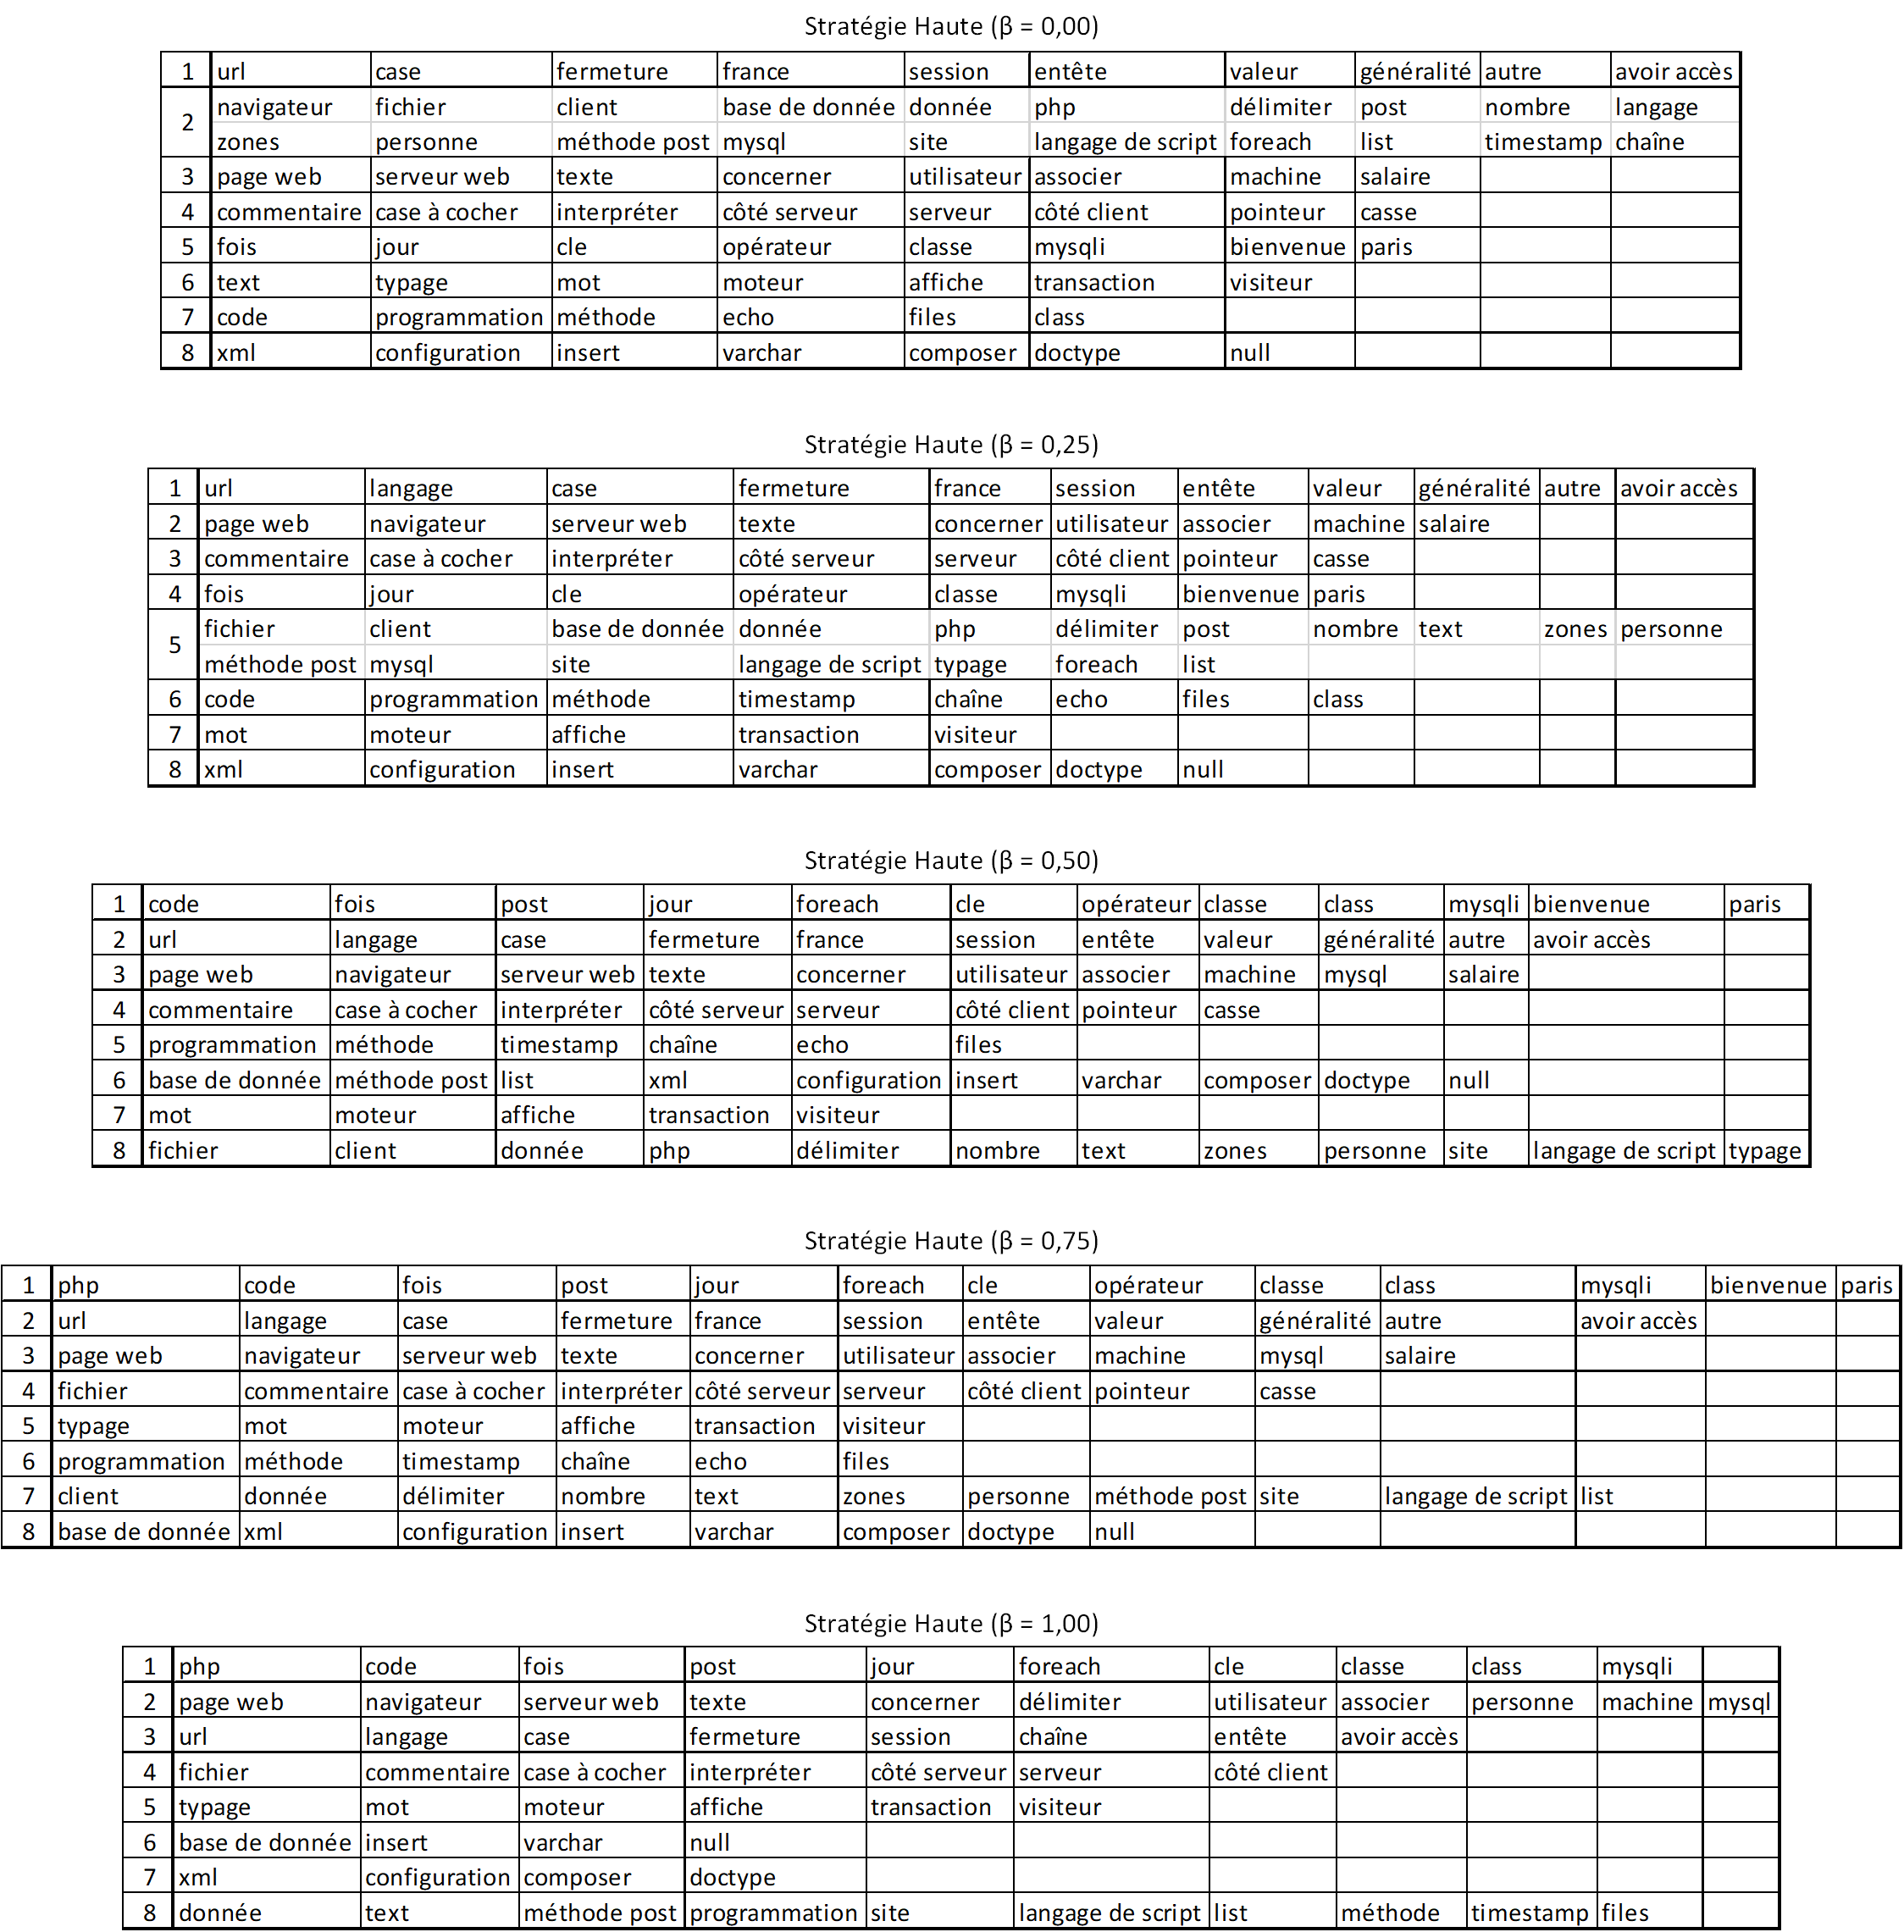
\includegraphics[scale=0.7]{4-Experiences/images/cas-1/clusters-S=H.png}
}
\caption{Clusters issus de la stratégie \textit{Haute} pour $ \beta $ de $0.00$ à $1.00$ par pas de $0.25$ pour le scénario n°1 référence}
\label{figure:4-cas-1-PII-ClustersStrategieHaute}
\end{figure}
%\end{figure*} % Figure flottante
% To use it : fig~\ref{label}



%\begin{figure*} % Figure flottante
\begin{figure}[htb!]
\centering
%\includegraphics[width=3in]{images/VerySmallModels_text.png}
%%\includegraphics[scale=0.6]{images/VerySmallModels_text.png}
\centerline{  % FORCE FIGURE OUTSIDE THE MARGIN !!! BUT STILL CENTERING !!!
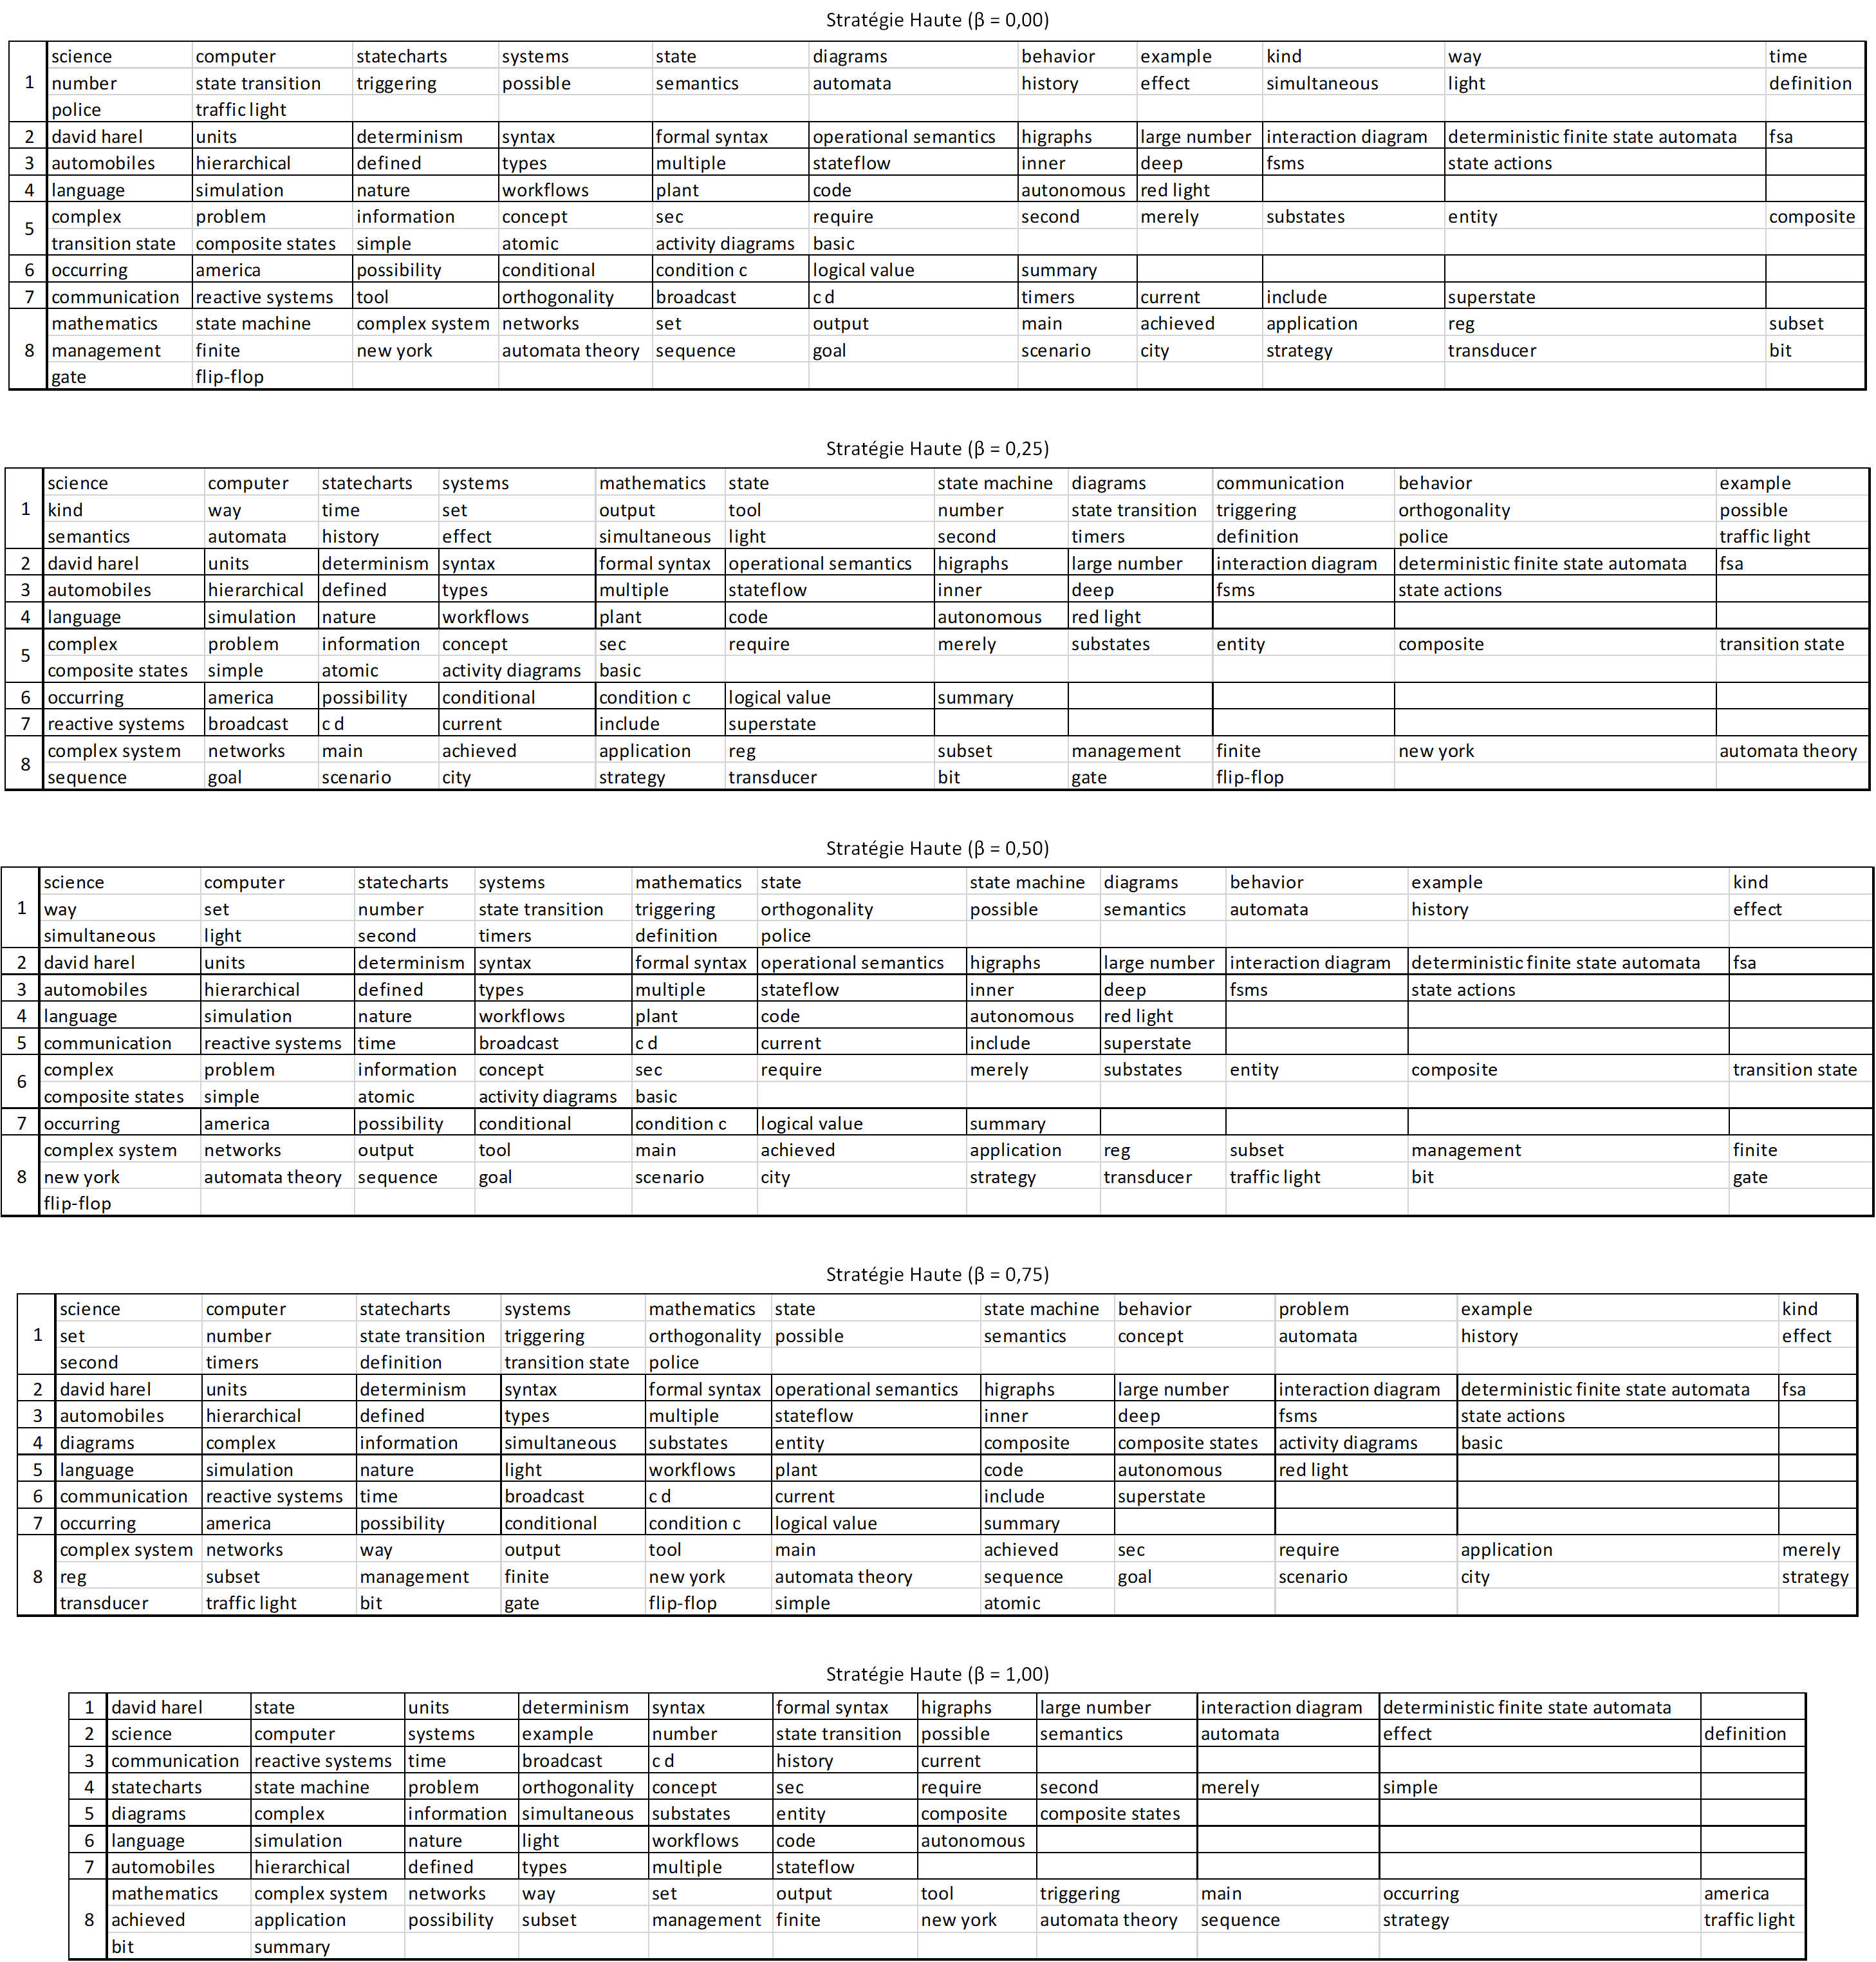
\includegraphics[scale=0.55]{4-Experiences/images/cas-6/clusters-Statecharts-S=H.png}
}
\caption{Clusters issus de la stratégie \textit{Haute} pour $ \beta $ de $0.00$ à $1.00$ par pas de $0.25$ pour le scénario n°5}
\label{figure:4-cas-6-PII-ClustersStrategieHaute}
\end{figure}
%\end{figure*} % Figure flottante
% To use it : fig~\ref{label}





%%%%%%%%%%%%%%%%%%%%%%%%%%%%%%%%%%%%%%%%%%%%
\clearpage % Clean for pictures and tables %
\newpage   % Clean for pictures and tables %
%%%%%%%%%%%%%%%%%%%%%%%%%%%%%%%%%%%%%%%%%%%%

%%%%%%%%%%%%%%%%%%%%%%%%%%%%%%%%%%%%%%%%%%%%%%%%%%%%%%%%%

\subsection{Validation fonctionnelle}
\label{subsection:Evaluation:DeroulementExperimentations:ValidationFonctionnelle}

Nous présentons maintenant les résultats bruts pour la validation fonctionnelle.
Comme indiqué dans le protocole présenté en section~\ref{section:Evaluation:ProtocoleEvaluation}, nous présentons tout d'abord les graphes d'impact mutuel formés avec les différents scénarios, puis les clusters de termes pour chacun des scénarios.
Le scénario n°2 visant à vérifier la résistance au bruit, et le scénario n°4 visant à comparer l'écart en cas de corrections, nous ne nous intéressons qu'aux graphes d'impact mutuel dans ces cas.
Les réponses de 5 informaticiens sont également présentées : les clusters qu'ils ont tout d'abord construits, puis leurs avis concernant les clusters produits par le cas de référence.



\subsubsection{Graphes d'impact mutuel (PII.2)}
\label{subsubsection:Evaluation:DeroulementExperimentations:ValidationFonctionnelle:GraphesImpactMutuel}

Le graphe d'impact mutuel permet à un enseignant d'obtenir une vue d'ensemble des supports de cours insérés et leurs termes afin de disposer d'une carte des notions les plus récurrentes et des documents partageant le plus ces notions.
La stratégie \textit{Directe} est employée pour générer le treillis de Galois (voir sous-section~\ref{subsubsection:CREA:PII.1.d-treillis}) étant donné qu'elle conserve l'ensemble des termes présents et permet donc d'avoir la vue la plus complète possible.
Pour rappel, le treillis généré permet de construire la matrice d'impact mutuel (voir sous-section~\ref{subsubsection:CREA:PII.1.e-metriquestreillis}) qui est illustrée par le graphe d'impact mutuel.
Le graphe d'impact mutuel est construit sur Gephi~\cite{bastian2009gephi} avec l'algorithme de spatialisation \textit{Force Atlas} en insérant une \textit{force de répulsion} entre \textit{1.000} et \textit{15.000} (selon le nombre de supports insérés), ainsi qu'une \textit{force d'attraction} entre \textit{5} et \textit{10} (pour la même raison).
Les figures~\ref{figure:4-cas-1-PII-GrapheDezoom-1} et~\ref{figure:4-cas-1-PII-GrapheDezoom-2} illustrent le graphe généré et la répartition concentrique des termes selon leur degré pour le scénario n°1.
Les cercles les plus extérieurs contiennent les termes connectés à peu de cours, à l'inverse, l'ensemble central en rouge contient les termes connectés aux 9 cours.

\bigskip

Dans le scénario n°1, en observant de plus près l'ensemble central on peut y lire les termes \textit{post}, \textit{méthode post}, \textit{nombre}, \textit{langage}, \textit{donnée}, \textit{fichier}, \textit{code}, \textit{php}, \textit{navigateur}, \textit{site}.
Dans le cadre de supports de cours abordant le développement web en PHP, ces termes sont très pertinents.
Seuls \og \textit{langage} \fg et éventuellement \og \textit{nombre} \fg semblent moins techniques, mais peuvent tout de même s'insérer dans le cadre de la gestion \textit{multi-lingue} d'un site ou du \textit{langage de programmation} PHP, ainsi que du type de données \textit{entier} ou \textit{integer}.
Les termes en orange (donc connectés à 8 des 9 cours) sont eux aussi adaptés : \og \textit{base de données} \fg , \og \textit{foreach} \fg , \og \textit{méthode} \fg .
En jaune (les termes connectés à 7 cours), on retrouve également des termes pertinents : \og \textit{serveur web} \fg , \og \textit{client} \fg , \og \textit{langage de script} \fg .
De même sur les termes en vert (connectés à 6 cours) : \og \textit{mysql} \fg , \og \textit{session} \fg , \og \textit{switch} \fg .
Plus on s'éloigne de l'ensemble central, plus on retrouve de termes peu adaptés à la construction d'un syllabus, voire, n'ont aucun sens par rapport au sujet.
Typiquement, les n\oe{}uds les plus éloignés contiennent le bruit non effacé par les précédentes étapes de nettoyage.

\bigskip

En comparant ensemble central avec les termes uniques retenus dans la matrice générée par la stratégie \textit{Haute}, on remarque que ces termes sont pour la grande majorité connectés à au moins 5 cours.
Plusieurs termes sont néanmoins absents, mais ceux-ci peuvent soit être sous-entendus par d'autres termes présents (\og \textit{sql} \fg pouvant être retrouvé via \og \textit{mysql} \fg par hyponymie, ou encore \og \textit{constructeur} \fg pouvant être retrouvé via \og \textit{classe} \fg par hyperonymie), soit sont des notions très spécifiques (\og \textit{switch} \fg et d'autres termes liés au langage de développement lui-même, donc des notions peu adaptées à une vision d'ensemble d'un cours).
La stratégie \textit{Haute} reflète cet ensemble central et les principales notions abordées dans les différents supports de cours.

\bigskip

%\begin{figure*} % Figure flottante
\begin{figure}[htb!]
\centering
%\includegraphics[width=3in]{images/VerySmallModels_text.png}
%%\includegraphics[scale=0.6]{images/VerySmallModels_text.png}
\centerline{  % FORCE FIGURE OUTSIDE THE MARGIN !!! BUT STILL CENTERING !!!
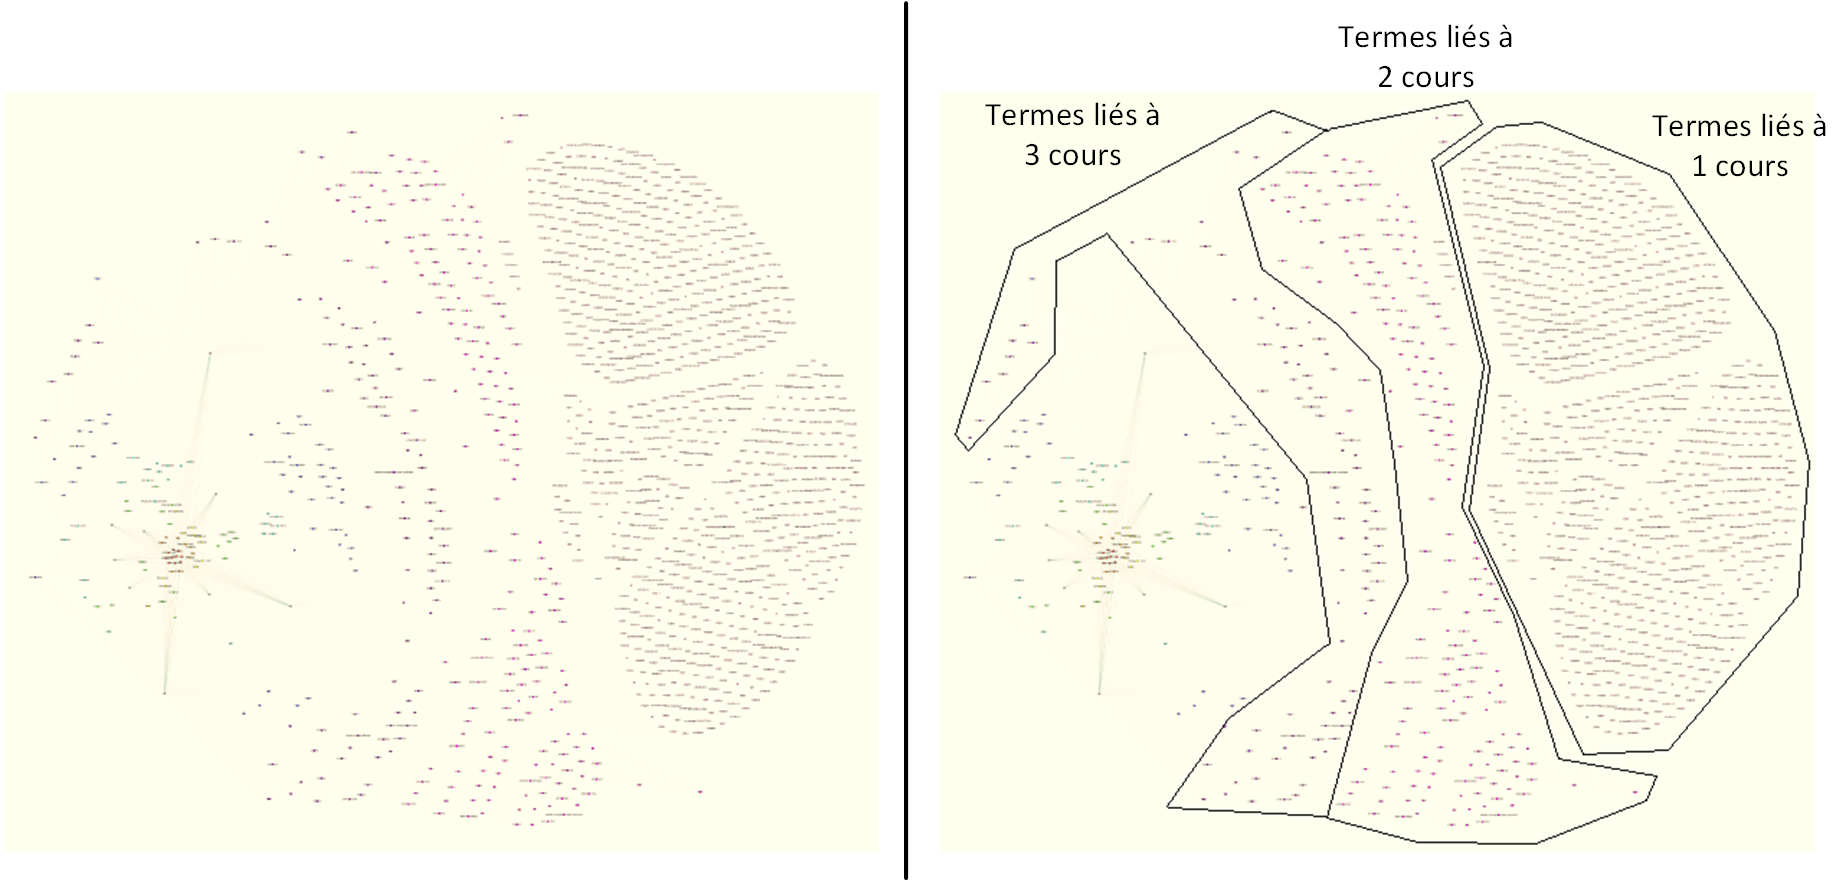
\includegraphics[scale=0.75]{4-Experiences/images/cas-1/Graphe-Directe-Explications.png}
}
\caption{Graphe d'impact mutuel des 9 cours [scénario n°1] : Vision d'ensemble éloignée et annotations}
\label{figure:4-cas-1-PII-GrapheDezoom-1}
\end{figure}
%\end{figure*} % Figure flottante
% To use it : fig~\ref{label}


%\begin{figure*} % Figure flottante
\begin{figure}[htb!]
\centering
%\includegraphics[width=3in]{images/VerySmallModels_text.png}
%%\includegraphics[scale=0.6]{images/VerySmallModels_text.png}
\centerline{  % FORCE FIGURE OUTSIDE THE MARGIN !!! BUT STILL CENTERING !!!
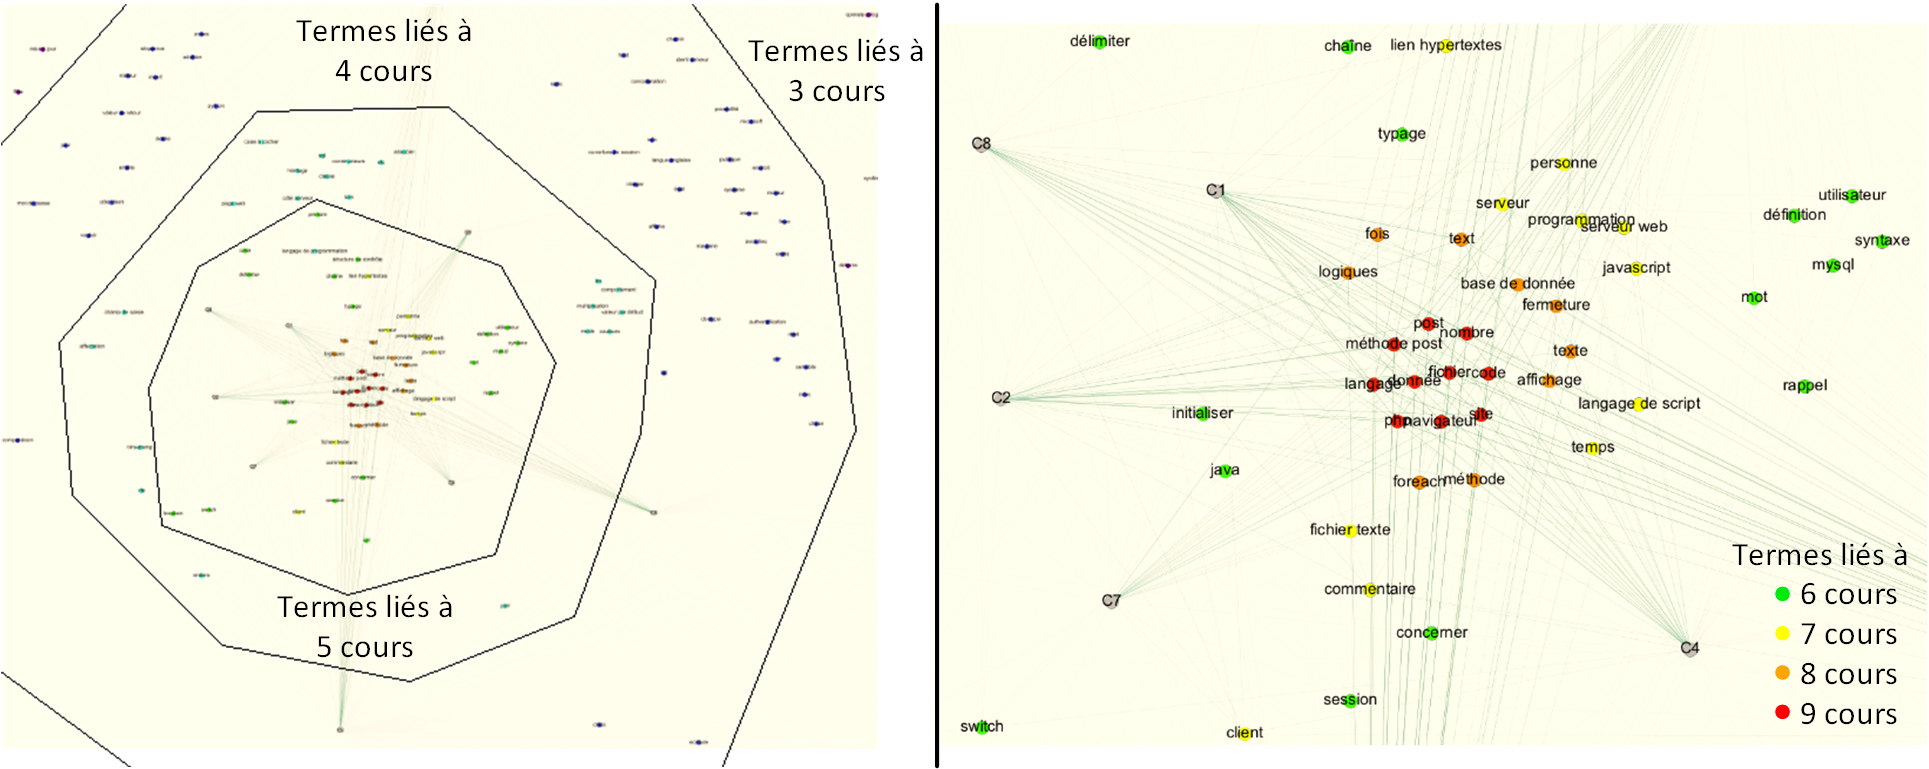
\includegraphics[scale=0.75]{4-Experiences/images/cas-1/Graphe-Directe-ExplicationsCore.png}
}
\caption{Graphe d'impact mutuel des 9 cours [scénario n°1] : Vision d'ensemble rapprochée et annotations}
\label{figure:4-cas-1-PII-GrapheDezoom-2}
\end{figure}
%\end{figure*} % Figure flottante
% To use it : fig~\ref{label}



%\begin{figure*} % Figure flottante
\begin{figure}[htb!]
\centering
%\includegraphics[width=3in]{images/VerySmallModels_text.png}
%%\includegraphics[scale=0.6]{images/VerySmallModels_text.png}
\centerline{  % FORCE FIGURE OUTSIDE THE MARGIN !!! BUT STILL CENTERING !!!
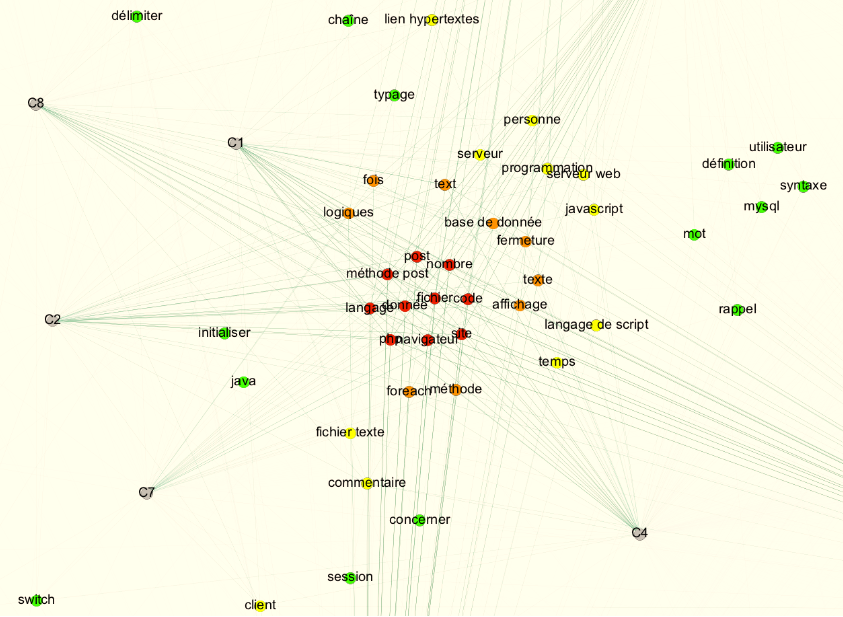
\includegraphics[scale=0.65]{4-Experiences/images/cas-1/graphe-Directe-core-zoom.png}
}
\caption{Graphe d'impact mutuel des 9 cours [scénario n°1] : Zoom sur l'ensemble central}
\label{figure:4-cas-1-PII-GrapheCoreZoom}
\end{figure}
%\end{figure*} % Figure flottante
% To use it : fig~\ref{label}


\newpage

L'ensemble central correspondant à ce qu'un enseignant s'attend à extraire de supports de cours de PHP, celui-ci peut évaluer la qualité des supports (quelles notions souhaite-t-il retrouver ou éviter, quelle distance maximale entre les supports accepte-t-il, ...).
Une analyse sur les supports de cours est illustrée par la figure~\ref{figure:4-cas-1-PII-GrapheCoursesZoom}.
On observe surtout que les supports au format texte sont les plus éloignés de l'ensemble central.
Les supports au format diapositives sont au contraire plus rapprochés de l'ensemble central.
Comme précédemment indiqué, cette différence peut s'expliquer par la plus forte quantité de vocabulaire employée dans les supports au format texte, par rapport au format diapositives.
Les supports au format texte disposant de beaucoup plus de termes uniques, ces derniers forment de grands ensembles dédiés à chacun des supports.
Ces ensembles étaient déjà sous-entendus dans le tableau~\ref{table:4-cas-1-PI-StatistiquesTermesUniquesPhaseI} grâce aux stratégies filtrant de nombreux termes selon leurs fréquences, et sont maintenant visibles sur le graphe d'impact mutuel.



%\begin{figure*} % Figure flottante
\begin{figure}[htb!]
\centering
%\includegraphics[width=3in]{images/VerySmallModels_text.png}
%%\includegraphics[scale=0.6]{images/VerySmallModels_text.png}
\centerline{  % FORCE FIGURE OUTSIDE THE MARGIN !!! BUT STILL CENTERING !!!
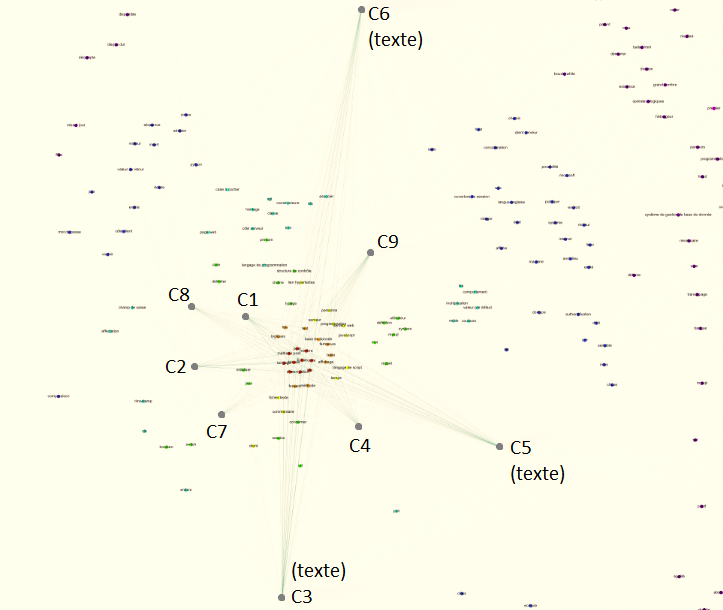
\includegraphics[scale=0.7]{4-Experiences/images/cas-1/graphe-Directe-core-courses-written.png}
}
\caption{Graphe d'impact mutuel des 9 cours [scénario n°1] : Zoom sur le positionnement des cours}
\label{figure:4-cas-1-PII-GrapheCoursesZoom}
\end{figure}
%\end{figure*} % Figure flottante
% To use it : fig~\ref{label}




%%%%%%%%%%%%%%%%%%%%%%%%%%%%%%%%%%%%%%%%%%%%
\clearpage % Clean for pictures and tables %
\newpage   % Clean for pictures and tables %
%%%%%%%%%%%%%%%%%%%%%%%%%%%%%%%%%%%%%%%%%%%%


%%%%%%%%%%%%%%%%%%%%%%%%%%%%%%%%%%%%%%
% SCENARIO N°2
%%%%%%%%%%%%%%%%%%%%%%%%%%%%%%%%%%%%%%

Le scénario n°2 vise à insérer un support de cours traitant d'un autre sujet.
Nous nous intéressons donc aux variations entre les graphiques du scénario n°1 et celui-ci.
La figure~\ref{figure:4-cas-2-PII-GrapheDezoom} illustre le graphe d'impact mutuel dans son ensemble.
La figure~\ref{figure:4-cas-2-PII-GrapheCoreZoom} illustre l'ensemble central.
Enfin, la figure~\ref{figure:4-cas-2-PII-GrapheCoursesZoom} illustre le positionnement des documents.

\bigskip

Dans l'ensemble central, les termes les plus fréquents (en rouge) sont maintenant \textit{donnée}, \textit{code}, \textit{nombre}, \textit{fichier}, \textit{langage}, \textit{méthode post}, \textit{site}, \textit{navigateur}, \textit{post}.
En comparant avec la liste précédente (figure~\ref{figure:4-cas-1-PII-GrapheCoreZoom}), on peut voir l'unique différence suivante : \textit{donnée}, \textit{code}, \textit{nombre}, \textit{fichier}, \textit{langage}, \textit{méthode post}, \textit{site}, \textit{navigateur}, \textit{post}, \sout{\textit{php}}.
Celle-ci est confirmée par le contenu du cours de Java abordant les notions sus-citées, excepté PHP.
Le terme \textit{php} est maintenant coloré en orange (donc relié à tous les cours, sauf 1) mais est le plus éloigné de la communauté centrale par rapport à tous les autres noe{}ds oranges : il se retrouve à la même distance que les n\oe{}uds jaunes (reliés à tous les cours, sauf 2) voire à la même distance que certains verts clairs (reliés à tous les cours, sauf 3).
On s'aperçoit que PHP n'est pas ce qui unit l'ensemble des supports de cours, mais bien les notions générales de programmation, et particulièrement ceux du développement web.



\vfill
\hspace{0pt}

%\begin{figure*} % Figure flottante
\begin{figure}[htb!]
\centering
%\includegraphics[width=3in]{images/VerySmallModels_text.png}
%%\includegraphics[scale=0.6]{images/VerySmallModels_text.png}
\centerline{  % FORCE FIGURE OUTSIDE THE MARGIN !!! BUT STILL CENTERING !!!
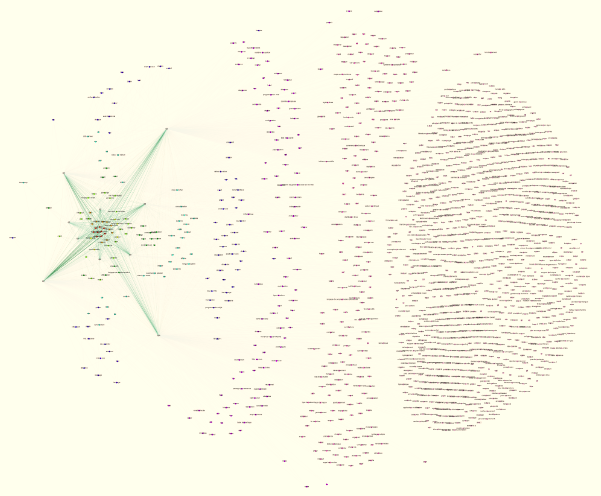
\includegraphics[scale=0.8]{4-Experiences/images/cas-2/graphe-Directe-dezoom.png}
}
\caption{Graphe d'impact mutuel des 10 cours [scénario n°2] : Vision d'ensemble éloignée}
\label{figure:4-cas-2-PII-GrapheDezoom}
\end{figure}
%\end{figure*} % Figure flottante
% To use it : fig~\ref{label}

\hspace{0pt}
\vfill



%%%%%% ESTHETIQUE
\clearpage
%%%%%% FIN ESTHETIQUE


%\begin{figure*} % Figure flottante
\begin{figure}[htb!]
\centering
%\includegraphics[width=3in]{images/VerySmallModels_text.png}
%%\includegraphics[scale=0.6]{images/VerySmallModels_text.png}
\centerline{  % FORCE FIGURE OUTSIDE THE MARGIN !!! BUT STILL CENTERING !!!
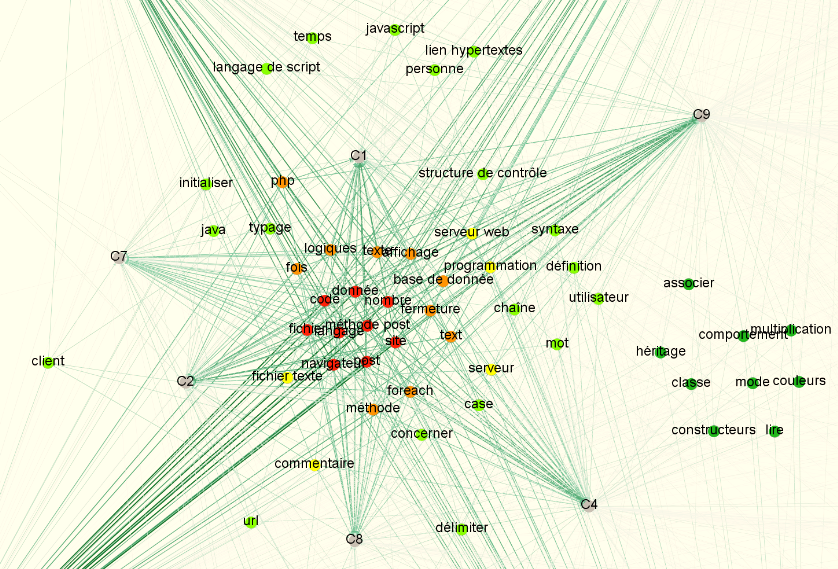
\includegraphics[scale=0.65]{4-Experiences/images/cas-2/graphe-Directe-core-zoom.png}
}
\caption{Graphe d'impact mutuel des 9 cours [scénario n°2] : Zoom sur l'ensemble central}
\label{figure:4-cas-2-PII-GrapheCoreZoom}
\end{figure}
%\end{figure*} % Figure flottante
% To use it : fig~\ref{label}

\bigskip

En observant le placement des cours sur la figure~\ref{figure:4-cas-2-PII-GrapheCoursesZoom}, on s'aperçoit que le cours de Java (CJA) est éloigné de l'ensemble central, au moins autant que C6.
Là où C3 et C5 étaient éloignés de l'ensemble central dans le cas n°1 (voir figure~\ref{figure:4-cas-1-PII-GrapheCoursesZoom}), ils apparaissent maintenant plus proches.
L'introduction d'un support de cours éloigné a contribué à partiellement rapprocher certains cours qui jusque là pouvaient paraitre anormalement éloignés.
Un enseignant s'apercevra donc inévitablement que les supports C6 et CJA devraient être vérifiés de plus près pour s'assurer de leur rapport avec le sujet qu'il souhaite enseigner.
Selon l'éloignement sémantique des supports, on peut supposer que la distance dans le graphe sera comparable : insérer un cours de philosophie risque d'être extrêmement éloigné et donc de rapprocher tous les autres cours (on peut néanmoins opposer l'idée qu'un enseignant n'insèrera pas de documents totalement hors sujet).
Chaque support éloigné doit donc être évalué manuellement pour vérifier sa pertinence, et éventuellement recalculer le graphe d'impact mutuel sans celui-ci.


%\begin{figure*} % Figure flottante
\begin{figure}[htb!]
\centering
%\includegraphics[width=3in]{images/VerySmallModels_text.png}
%%\includegraphics[scale=0.6]{images/VerySmallModels_text.png}
\centerline{  % FORCE FIGURE OUTSIDE THE MARGIN !!! BUT STILL CENTERING !!!
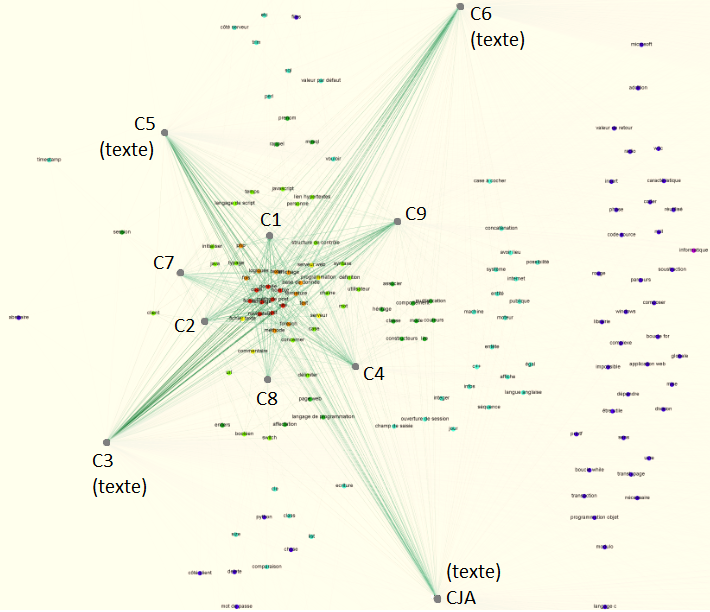
\includegraphics[scale=0.7]{4-Experiences/images/cas-2/graphe-Directe-core-courses-written.png}
}
\caption{Graphe d'impact mutuel des 10 cours [scénario n°2] : Zoom sur le positionnement des cours}
\label{figure:4-cas-2-PII-GrapheCoursesZoom}
\end{figure}
%\end{figure*} % Figure flottante
% To use it : fig~\ref{label}




%%%%%%%%%%%%%%%%%%%%%%%%%%%%%%%%%%%%%%%%%%%%
\clearpage % Clean for pictures and tables %
\newpage   % Clean for pictures and tables %
%%%%%%%%%%%%%%%%%%%%%%%%%%%%%%%%%%%%%%%%%%%%

%%%%%%%%%%%%%%%%%%%%%%%%%%%%%%%%%%%%%%
% SCENARIO N°3
%%%%%%%%%%%%%%%%%%%%%%%%%%%%%%%%%%%%%%

Le scénario n°3 vise à s'assurer du maintien des résultats précédents malgré le doublement du nombre de documents insérés par rapport au scénario n°1 (18 documents insérés contre seulement 9).
La figure~\ref{figure:4-cas-3-PII-GrapheDezoom} illustre le graphe d'impact mutuel dans son ensemble.
La figure~\ref{figure:4-cas-3-PII-GrapheCoreZoom} illustre l'ensemble central.
Enfin, la figure~\ref{figure:4-cas-3-PII-GrapheCoursesZoom} illustre le positionnement des documents.

\bigskip

Étant donné que le nombre de cours est doublé, le nombre de groupes de termes l'est lui aussi.
Comme nous l'avons observé pour le scénario n°1, chaque document dispose d'un ensemble de termes qui lui est propre : en doublant le nombre de documents, nous avons ajouté autant d'ensembles de termes uniques que de documents en plus.
On retrouve en haut à gauche l'ensemble central, puis plus bas vers la droite, chaque groupe de termes dont le nombre de connexions se réduit par itération jusqu'à 1.

\bigskip

En analysant l'ensemble central, illustré par la figure~\ref{figure:4-cas-3-PII-GrapheCoreZoom}, on trouve 6 termes reliés à l'ensemble des supports de cours : \textit{navigateur}, \textit{site}, \textit{fichier}, \textit{langage}, \textit{php}, \textit{code}.
Certains termes ont été légèrement déplacés plus en extérieur en perdant 1 relation par rapport au cas n°1 : \textit{nombre}, \textit{méthode post}, \textit{texte}, \textit{donnée}.
Visuellement, l'ensemble central est resté stable (peu de variation des termes), et le sujet principal est toujours correctement remonté par le graphe.
Enfin, les termes perdant 2 relations par rapport au cas n°1 (\textit{langage de script}, \textit{serveur web}, \textit{javascript}, \textit{serveur}, \textit{base de donnée}, \textit{text}) constituent eux aussi des notions importantes.
Les termes avec des degrés plus faibles restent néanmoins utiles pour un cours de développement web en PHP (ceux en vert et bleu).
On notera que quelques termes provoquant du bruit comme dans le cas n°1 (\textit{fois}, \textit{mot}, et \textit{définition} (qui peut éventuellement être interprété comme un \textit{define} de constante)) sont toujours présents.
Le doublement du nombre de documents n'a donc pas modifié le sujet central détecté par le graphe d'impact mutuel.



%\begin{figure*} % Figure flottante
\begin{figure}[htb!]
\centering
%\includegraphics[width=3in]{images/VerySmallModels_text.png}
%%\includegraphics[scale=0.6]{images/VerySmallModels_text.png}
\centerline{  % FORCE FIGURE OUTSIDE THE MARGIN !!! BUT STILL CENTERING !!!
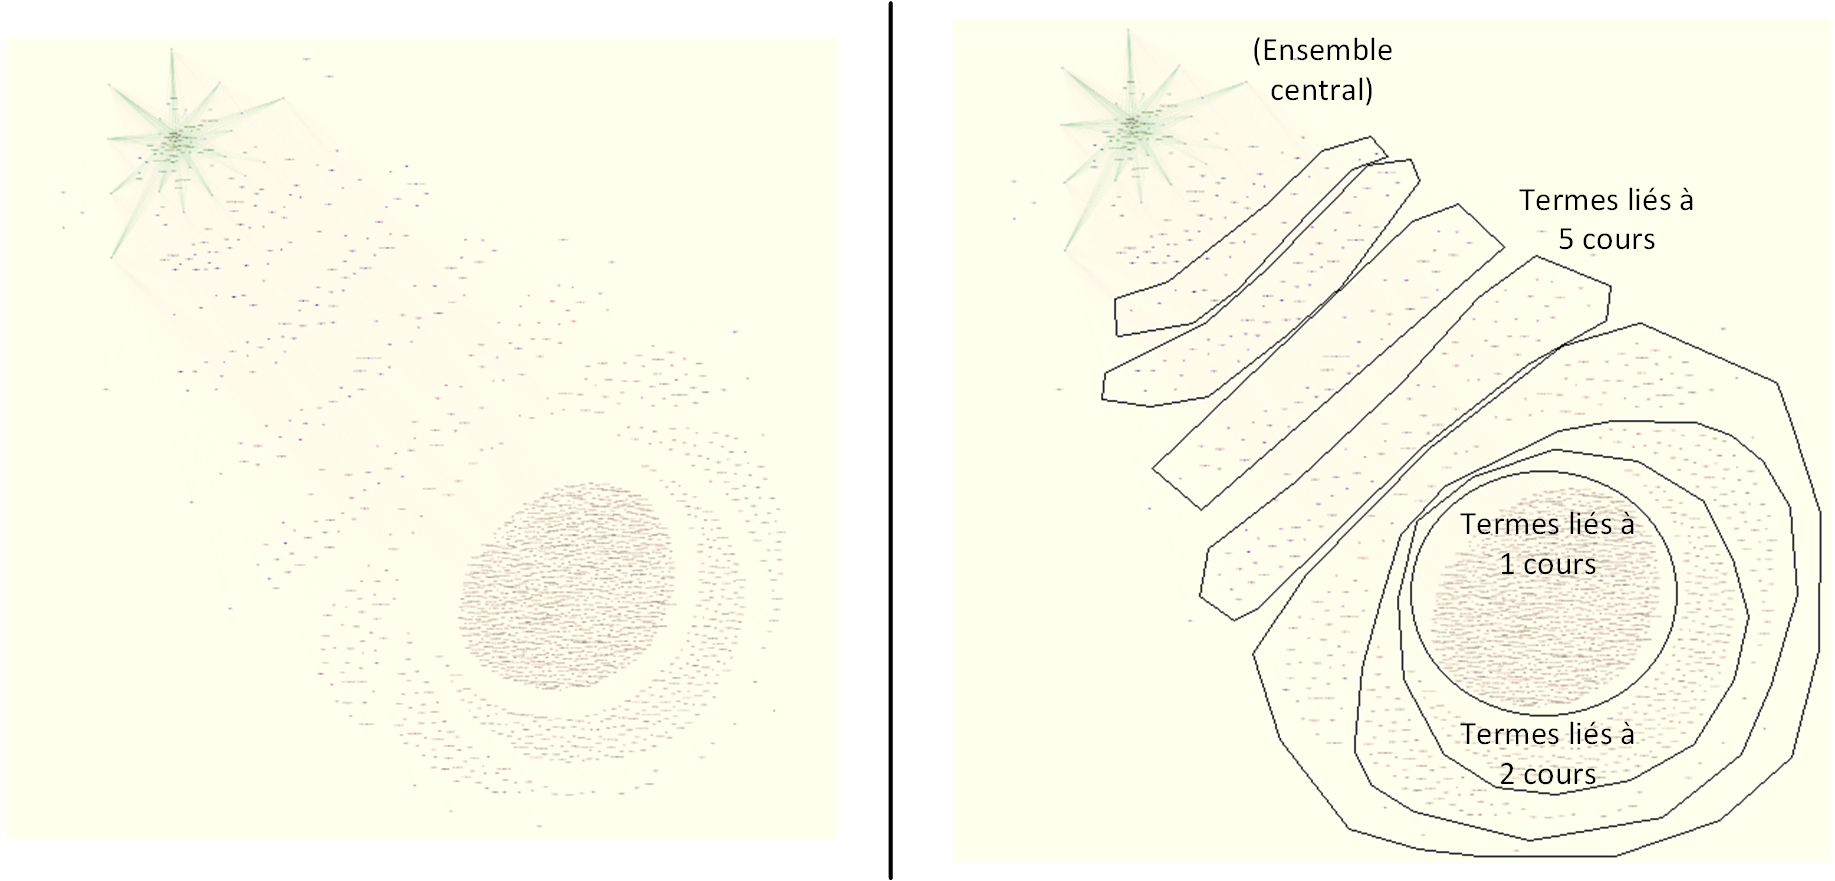
\includegraphics[scale=0.8]{4-Experiences/images/cas-3/Graphe-Directe-Explications.png}
}
\caption{Graphe d'impact mutuel des 18 cours [scénario n°3] : Vision d'ensemble éloignée et annotations}
\label{figure:4-cas-3-PII-GrapheDezoom}
\end{figure}
%\end{figure*} % Figure flottante
% To use it : fig~\ref{label}



L'ensemble central étant stable malgré le dédoublement du nombre de supports de cours insérés, nous nous intéressons maintenant à la pertinence des supports avec la figure~\ref{figure:4-cas-3-PII-GrapheCoursesZoom}.
En observant le positionnement des documents, on se rend compte que la plupart des supports forment eux aussi un ensemble homogène.
C6, qui était déjà éloigné dans les scénarios n°1 et n°2, est confirmé dans son éloignement, mais est rejoint par C11.
Les supports textes sont les plus éloignés.
C17, qui était le support avec le moins de mots parmi les supports au format texte, d'après le tableau~\ref{table:4-cas-1-PI-StatistiquesMotsTermesPhaseI}, se trouve éloigné comme les autres.


%\begin{figure*} % Figure flottante
\begin{figure}[htb!]
\centering
%\includegraphics[width=3in]{images/VerySmallModels_text.png}
%%\includegraphics[scale=0.6]{images/VerySmallModels_text.png}
\centerline{  % FORCE FIGURE OUTSIDE THE MARGIN !!! BUT STILL CENTERING !!!
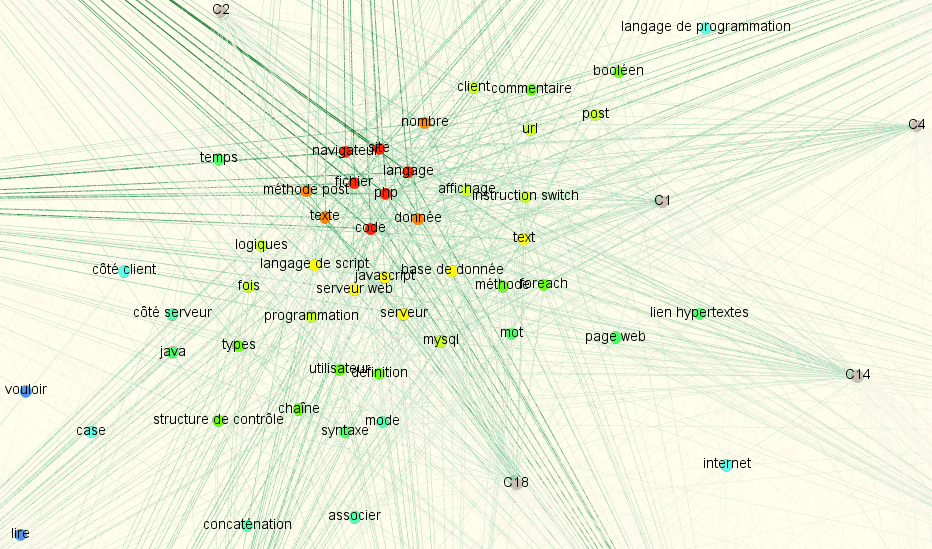
\includegraphics[scale=0.65]{4-Experiences/images/cas-3/graphe-Directe-core-zoom.png}
}
\caption{Graphe d'impact mutuel des 18 cours [scénario n°3] : Zoom sur l'ensemble central}
\label{figure:4-cas-3-PII-GrapheCoreZoom}
\end{figure}
%\end{figure*} % Figure flottante
% To use it : fig~\ref{label}



%\begin{figure*} % Figure flottante
\begin{figure}[htb!]
\centering
%\includegraphics[width=3in]{images/VerySmallModels_text.png}
%%\includegraphics[scale=0.6]{images/VerySmallModels_text.png}
\centerline{  % FORCE FIGURE OUTSIDE THE MARGIN !!! BUT STILL CENTERING !!!
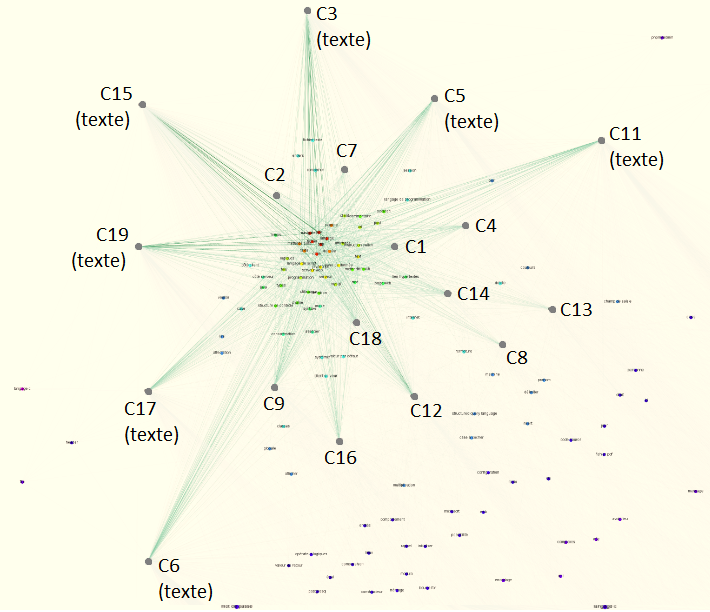
\includegraphics[scale=0.7]{4-Experiences/images/cas-3/graphe-Directe-core-courses-written.png}
}
\caption{Graphe d'impact mutuel des 18 cours [scénario n°3] : Zoom sur le positionnement des cours}
\label{figure:4-cas-3-PII-GrapheCoursesZoom}
\end{figure}
%\end{figure*} % Figure flottante
% To use it : fig~\ref{label}


%%%%%%%%%%%%%%%%%%%%%%%%%%%%%%%%%%%%%%%%%%%%
\clearpage % Clean for pictures and tables %
\newpage   % Clean for pictures and tables %
%%%%%%%%%%%%%%%%%%%%%%%%%%%%%%%%%%%%%%%%%%%%



%%%%%%%%%%%%%%%%%%%%%%%%%%%%%%%%%%%%%%%%%%%%%%%%%%
% SCENARIO N°4
%%%%%%%%%%%%%%%%%%%%%%%%%%%%%%%%%%%%%%%%%%%%%%%%%%

Le scénario n°4 vise à vérifier que la méthode est fonctionnellement correcte en s'assurant que l'amélioration des documents en entrée produit un graphe d'impact mutuel reflétant ces améliorations.
Pour cela, le document C6 (qui était éloigné sur les précédents graphes d'impact mutuel) est successivement corrigé.
Ce scénario étudie six versions successives :
\begin{enumerate}
\item Corpus documentaire des 7 supports de cours au format texte traitant de PHP
\item Suppression du chapitre dédié aux projets (pages 93 - 150, soit 103 pages restantes) dans C6
\item Suppression du chapitre déclaré comme \og hors programme \fg (pages 41 - 65, soit 79 pages restantes) dans C6
\item Ajout du support Java à la version initiale contenant les 7 supports au format texte
\item Ajout du support Java à la version sans projets
\item Ajout du support Java à la version sans projets ni \og hors programme \fg
\end{enumerate}

\bigskip

Le premier graphe d'impact mutuel présentant les 7 supports de cours originaux au format texte est représenté par la figure~\ref{figure:4-cas-final-1-PII-GrapheCoreZoom}.
On constate que C6 est effectivement le document le plus éloigné de l'ensemble central.
On notera que C5, C11, et C15 sont également assez éloignés, mais moins que C6.

\vfill
\hspace{0pt}

\begin{figure}[htb!]
\centering
\centerline{  % FORCE FIGURE OUTSIDE THE MARGIN !!! BUT STILL CENTERING !!!  % 0.75
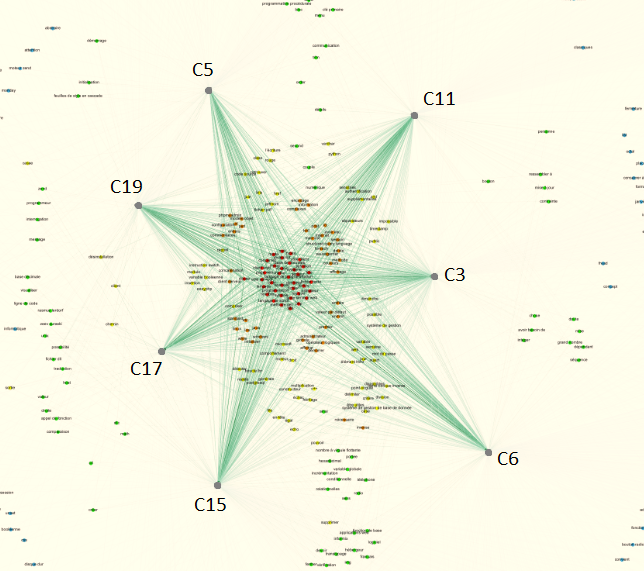
\includegraphics[scale=0.69]{4-Experiences/images/cas-final/1-Full-Text-PHP_core-courses-written.png}
}
\caption{Graphe d'impact mutuel des 7 supports de cours originaux au format texte traitant de PHP [scénario n°4] : Zoom sur le positionnement des documents}
\label{figure:4-cas-final-1-PII-GrapheCoreZoom}
\end{figure}

\hspace{0pt}
\vfill

\clearpage

Le deuxième graphe d'impact mutuel présentant les 7 supports de cours au format texte, mais dans lequel C6 a été corrigé en lui retirant le chapitre sur les projets étudiants, est représenté par la figure~\ref{figure:4-cas-final-2-PII-GrapheCoreZoom}.
On constate que C6 s'est très nettement rapproché de l'ensemble central, et que les documents les plus éloignés sont devenus C5, C11, et C15.
La correction a donc eu un impact positif pour le document C6 : celui-ci est maintenant beaucoup plus proche du sujet présenté dans le corpus.
Du point de vue global, le graphe est visuellement plus équilibré : C6 étant devenu assez proche de l'ensemble central, les autres documents sont un peu plus difficiles à distinguer au niveau de leurs distances avec l'ensemble central.

\vfill
\hspace{0pt}

\begin{figure}[htb!]
\centering
\centerline{  % FORCE FIGURE OUTSIDE THE MARGIN !!! BUT STILL CENTERING !!!
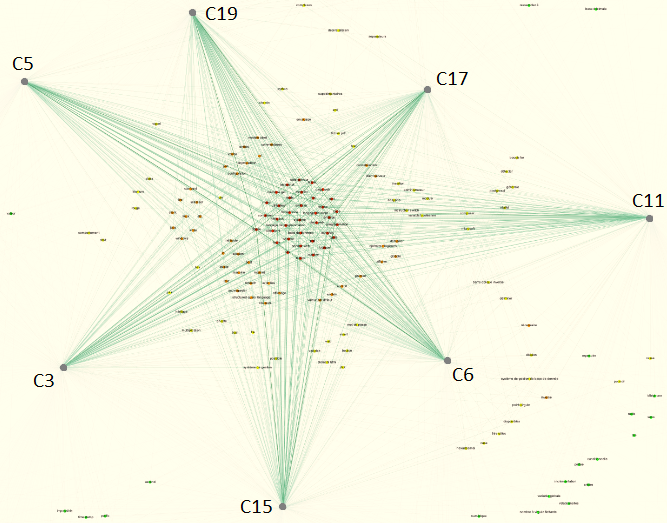
\includegraphics[scale=0.75]{4-Experiences/images/cas-final/2-Full-Text-C+noP-PHP_core-courses-written.png}
}
\caption{Graphe d'impact mutuel des 7 supports de cours au format texte traitant de PHP, dont C6 a été corrigé en retirant le chapitre traitant des projets étudiants [scénario n°4] : Zoom sur le positionnement des documents}
\label{figure:4-cas-final-2-PII-GrapheCoreZoom}
\end{figure}

\hspace{0pt}
\vfill

\clearpage

Le troisième graphe d'impact mutuel présentant les 7 supports de cours au format texte, mais dans lequel C6 a été corrigé en lui retirant le chapitre sur les projets étudiants ainsi que le chapitre déclaré comme \og hors programme \fg, est représenté par la figure~\ref{figure:4-cas-final-3-PII-GrapheCoreZoom}.
On constate que C6 s'est encore un peu plus rapproché de l'ensemble central, et au contraire, C11 est devenu le document le plus éloigné de l'ensemble central.
La correction a donc encore eu un impact positif pour le document C6, mais le graphe s'est visuellement déséquilibré en repoussant particulièrement C11.

\vfill
\hspace{0pt}

\begin{figure}[htb!]
\centering
\centerline{  % FORCE FIGURE OUTSIDE THE MARGIN !!! BUT STILL CENTERING !!!
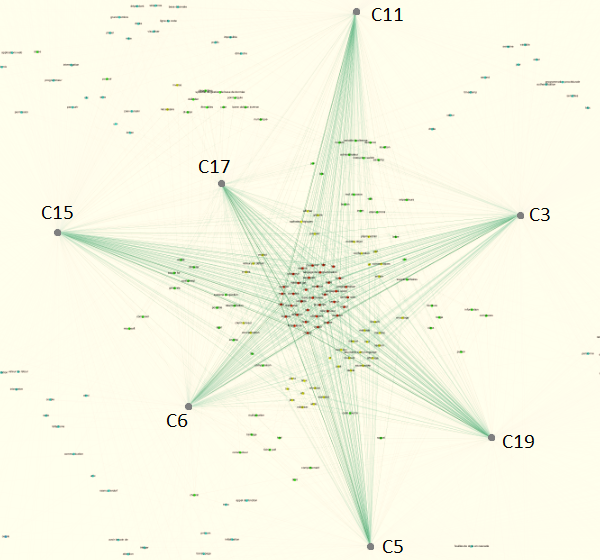
\includegraphics[scale=0.8]{4-Experiences/images/cas-final/3-Full-Text-noC+noP-PHP_core-courses-written.png}
}
\caption{Graphe d'impact mutuel des 7 supports de cours au format texte traitant de PHP, dont C6 a été corrigé en retirant le chapitre traitant des projets étudiants ainsi que le chapitre hors programme [scénario n°4] : Zoom sur le positionnement des documents}
\label{figure:4-cas-final-3-PII-GrapheCoreZoom}
\end{figure}

\hspace{0pt}
\vfill

\clearpage

Le quatrième graphe d'impact mutuel présentant les 7 supports de cours au format texte ainsi que le support Java (CJA), est représenté par la figure~\ref{figure:4-cas-final-4-PII-GrapheCoreZoom}.
On remarque que C6 et CJA sont les plus éloignés, particulièrement C6.
Bien que C6 traite de PHP, l'excès de chapitres hors sujet (et particulièrement la quantité de termes) en fait un document beaucoup plus éloigné des autres.

\vfill
\hspace{0pt}

\begin{figure}[htb!]
\centering
\centerline{  % FORCE FIGURE OUTSIDE THE MARGIN !!! BUT STILL CENTERING !!!
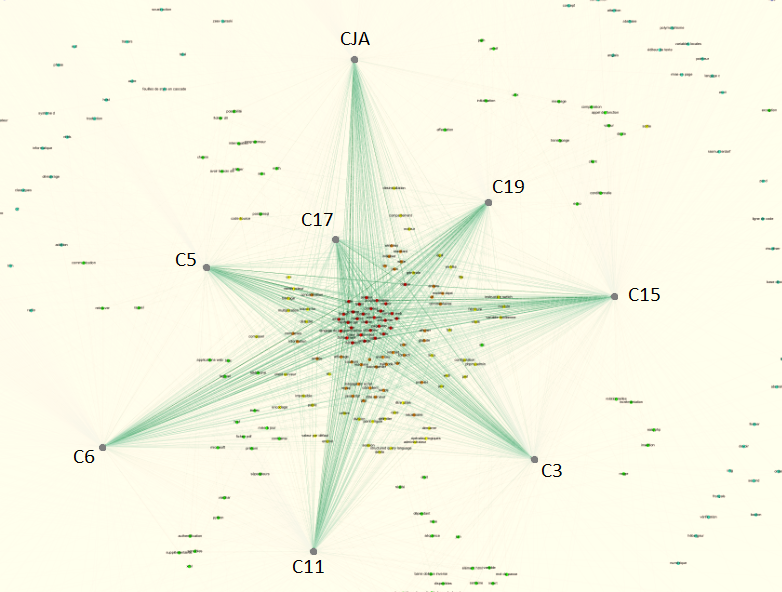
\includegraphics[scale=0.75]{4-Experiences/images/cas-final/4-Full-Text-PHP+Java_core-courses-written.png}
}
\caption{Graphe d'impact mutuel des 7 supports de cours au format texte traitant de PHP complétés du support Java [scénario n°4] : Zoom sur le positionnement des documents}
\label{figure:4-cas-final-4-PII-GrapheCoreZoom}
\end{figure}

\hspace{0pt}
\vfill

\clearpage

Le cinquième graphe d'impact mutuel présentant les 7 supports de cours au format texte ainsi que le support Java (CJA), mais dans lequel C6 a été corrigé en lui retirant le chapitre sur les projets étudiants, est représenté par la figure~\ref{figure:4-cas-final-5-PII-GrapheCoreZoom}.
On constate que C6 s'est très rapproché de l'ensemble central, mais seuls CJA et C11 sont devenus les plus éloignés.
Visuellement, la forme du graphe s'approche d'un parallélogramme, voire d'un losange : hormis CJA et C11, les autres documents sont presque équidistants de l'ensemble central (le cas parfait aurait évidemment été un cercle).
La correction de C6 a donc créé un corpus qui visuellement est beaucoup plus homogène que dans les autres cas.

\vfill
\hspace{0pt}

\begin{figure}[htb!]
\centering
\centerline{  % FORCE FIGURE OUTSIDE THE MARGIN !!! BUT STILL CENTERING !!!
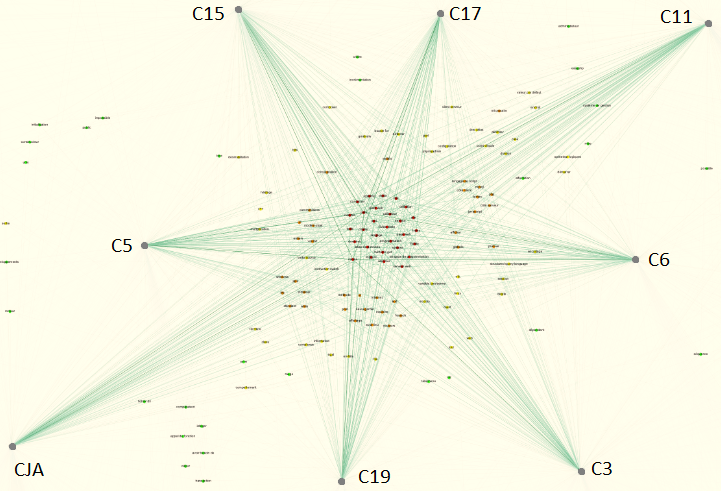
\includegraphics[scale=0.75]{4-Experiences/images/cas-final/5-Full-Text-C+noP-PHP+Java_core-courses-written.png}
}
\caption{Graphe d'impact mutuel des 7 supports de cours au format texte traitant de PHP complétés du support Java, dont C6 a été corrigé en retirant le chapitre traitant des projets étudiants [scénario n°4] : Zoom sur le positionnement des documents}
\label{figure:4-cas-final-5-PII-GrapheCoreZoom}
\end{figure}

\hspace{0pt}
\vfill

\clearpage

Le sixième graphe d'impact mutuel présentant les 7 supports de cours au format texte ainsi que le support Java (CJA), mais dans lequel C6 a été corrigé en lui retirant le chapitre sur les projets étudiants ainsi que le chapitre déclaré comme \og hors programme \fg, est représenté par la figure~\ref{figure:4-cas-final-6-PII-GrapheCoreZoom}.
On constate que C6 s'est nettement rapproché de l'ensemble central, et est devenu le document le plus proche.
C11 et CJA sont les plus éloignés, ainsi que C15.
La double correction a donc bien eu un effet sur le graphe, mais graphiquement, la forme aperçue dispose d'un sommet particulièrement décalé vers l'intérieur.

\vfill
\hspace{0pt}

\begin{figure}[htb!]
\centering
\centerline{  % FORCE FIGURE OUTSIDE THE MARGIN !!! BUT STILL CENTERING !!!
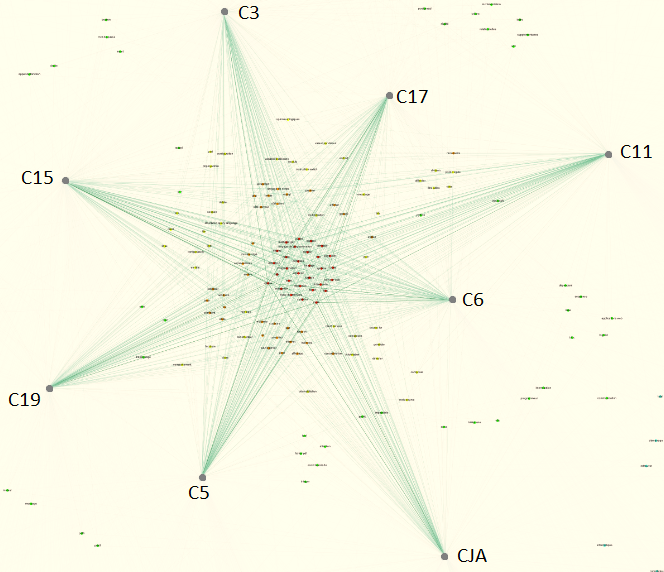
\includegraphics[scale=0.75]{4-Experiences/images/cas-final/6-Full-Text-noC+noP-PHP+Java_core-courses-written.png}
}
\caption{Graphe d'impact mutuel des 7 supports de cours au format texte traitant de PHP complétés du support Java, dont C6 a été corrigé en retirant le chapitre traitant des projets étudiants ainsi que le chapitre hors programme [scénario n°4] : Zoom sur le positionnement des documents}
\label{figure:4-cas-final-6-PII-GrapheCoreZoom}
\end{figure}

\hspace{0pt}
\vfill


%%%%%%%%%%%%%%%%%%%%%%%%%%%%%%%%%%%%%%%%%%%%
\clearpage % Clean for pictures and tables %
\newpage   % Clean for pictures and tables %
%%%%%%%%%%%%%%%%%%%%%%%%%%%%%%%%%%%%%%%%%%%%


%%%%%%%%%%%%%%%%%%%%%%%%%%%%%%%%%%%%%%%%%%%%%%%%%%
% SCENARIO N°5
%%%%%%%%%%%%%%%%%%%%%%%%%%%%%%%%%%%%%%%%%%%%%%%%%%

Le scénario n°5 vise à s'assurer que la méthode CREA fonctionne sur d'autres sujets d'intérêts, et dans une autre langue.
La figure~\ref{figure:4-cas-6-PII-GrapheCoreZoom} illustre l'ensemble central.
La figure~\ref{figure:4-cas-6-PII-GrapheCoursesZoom} illustre le positionnement des documents.

\bigskip

L'ensemble central du graphe d'impact mutuel, visible sur la figure~\ref{figure:4-cas-6-PII-GrapheCoreZoom}, présente seulement 2 termes communs à l'ensemble des 13 documents : \og \textit{statecharts} \fg et \og \textit{state machine} \fg.
Le sujet étudié est donc correctement détecté dans l'ensemble des documents.
On remarque que \og \textit{time} \fg est le troisième terme le plus connecté.
Celui-ci est lié aux exemples employant régulièrement ce terme (on peut citer l'exemple détaillant le fonctionnement d'une montre digitale), mais également au domaine lors de la gestion des transitions et évènements dans le temps.
Plusieurs autres termes importants du domaine sont visibles en périphérie du noyau en rouge : \og \textit{triggering} \fg, \og \textit{state transition} \fg, \og \textit{substates} \fg, \og \textit{process} \fg, \og \textit{diagrams} \fg, \og \textit{automata} \fg, \og \textit{semantics} \fg, \og \textit{systems} \fg, \og \textit{complex} \fg.
Bien que l'ensemble central soit plus éparse que nos précédents exemples, il n'en reste pas moins explicite et correct concernant le contenu des documents sélectionnés.

\bigskip

Concernant les 13 documents, la figure~\ref{figure:4-cas-6-PII-GrapheCoursesZoom} montre que les articles sont plus éloignés que les autres types de documents.
Les documents les plus éloignés sont aussi les plus longs en quantité de mots et de termes : A4 étant le chapitre de livre et A1 étant un article particulièrement long.
A2, A5, et C7 sont également parmi les plus gros en quantité de termes, par rapport aux cours composés de quelques centaines de termes.
L'article A3 est plus difficile à expliquer : sur la quantité de termes, il est comparable à C1, mais il se retrouve graphiquement presque aussi éloigné que A1 et A4.
Il s'agit d'un article \textbf{utilisant} les statecharts, mais détaillant également une étude de cas et quelques autres formalismes différents des statecharts.
Cette non spécialisation sur les statecharts, contrairement à l'ensemble des autres documents, pourrait être à l'origine de cet écart.


% ESTHETIQUE
\newpage



%\begin{figure*} % Figure flottante
\begin{figure}[htb!]
\centering
%\includegraphics[width=3in]{images/VerySmallModels_text.png}
%%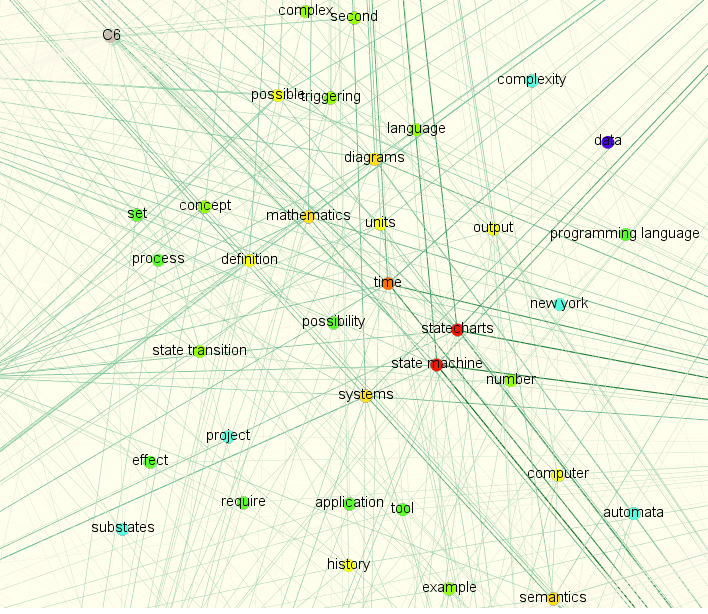
\includegraphics[scale=0.6]{images/VerySmallModels_text.png
\centerline{  % FORCE FIGURE OUTSIDE THE MARGIN !!! BUT STILL CENTERING !!!
\includegraphics[scale=0.6]{4-Experiences/images/cas-6/graphe-Statecharts-Directe-core-zoom.png}
%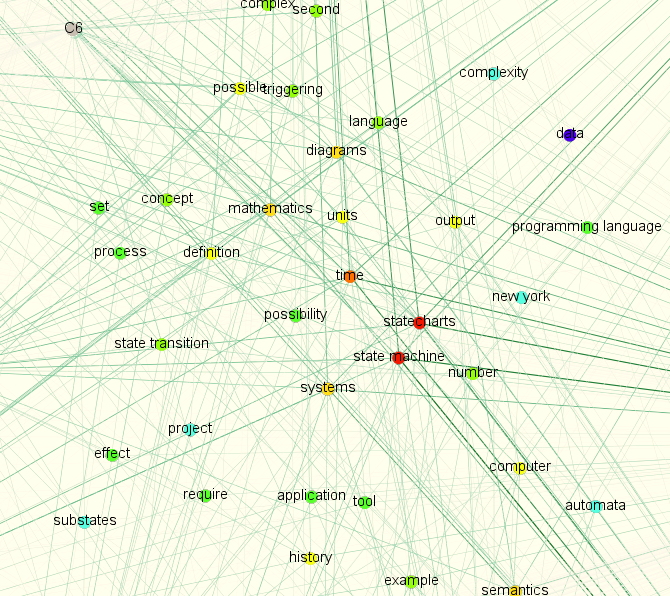
\includegraphics[scale=0.6]{4-Experiences/images/cas-6/graphe-Statecharts-Directe-core-zoom-recut.png}
}
\caption{Graphe d'impact mutuel des 8 cours et 5 articles sur les statecharts [scénario n°5] : Zoom sur l'ensemble central}
\label{figure:4-cas-6-PII-GrapheCoreZoom}
\end{figure}
%\end{figure*} % Figure flottante
% To use it : fig~\ref{label}


%\begin{figure*} % Figure flottante
\begin{figure}[htb!]
\centering
%\includegraphics[width=3in]{images/VerySmallModels_text.png}
%%\includegraphics[scale=0.6]{images/VerySmallModels_text.png}
\centerline{  % FORCE FIGURE OUTSIDE THE MARGIN !!! BUT STILL CENTERING !!!
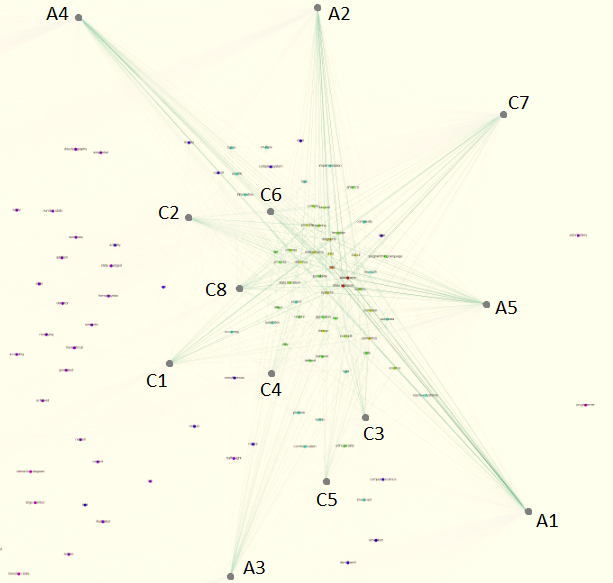
\includegraphics[scale=0.6]{4-Experiences/images/cas-6/graphe-Statecharts-Directe-core-courses-written.png}
%\includegraphics[scale=0.6]{4-Experiences/images/cas-6/graphe-Statecharts-Directe-core-courses-written-recut.png}
}
\caption{Graphe d'impact mutuel des 8 cours et 5 articles sur les statecharts [scénario n°5] : Zoom sur le positionnement des documents}
\label{figure:4-cas-6-PII-GrapheCoursesZoom}
\end{figure}
%\end{figure*} % Figure flottante
% To use it : fig~\ref{label}


%%%%%%%%%%%%%%%%%%%%%%%%%%%%%%%%%%%%%%%%%%%%
\clearpage % Clean for pictures and tables %
\newpage   % Clean for pictures and tables %
%%%%%%%%%%%%%%%%%%%%%%%%%%%%%%%%%%%%%%%%%%%%


%%%%%%%%%%%%%%%%%%%%%%%%%%%%%%%%%%%%%%%%%%%%%%%%%%%%%%%%%%%%%%%%%%%%%%%%%%%%%%%%%%%%%%%%%%%%%%%%%%%%%%%%%%%%%%%%%%%

\subsubsection{Clusters de termes (PII.3)}
\label{subsubsection:Evaluation:DeroulementExperimentations:ValidationFonctionnelle:Clusters}

Les supports étant en lien avec le sujet, et l'ensemble central illustrant ce sujet par l'intermédiaire de plusieurs termes, nous nous intéressons maintenant aux clusters générés avec la matrice de similarité conceptuelle.
Comme expliqué lors de la validation structurelle en~\ref{subsubsection:Evaluation:DeroulementExperimentations:ValidationStructurelle:ResultatsClustersS1}, il apparait que $ \beta = 1.00 $ est la valeur la plus adaptée pour générer des clusters pertinents pour un enseignant.
Nous générons donc les 8 clusters des scénarios n°1 et 3 comme illustré sur la figure~\ref{figure:4-cas-3-PII-ClustersStrategieHaute}, et les 8 clusters du scénario n°5 comme illustré sur la figure~\ref{figure:4-cas-6-PII-ClustersStrategieHaute-Beta-1}.

\bigskip


%%%%%%%%%%%%%%%%%%%%%%%%%%%%%%%%%%%%%%%%%%%%%%%%%%
% SCENARIOS N°1 ET 3
%%%%%%%%%%%%%%%%%%%%%%%%%%%%%%%%%%%%%%%%%%%%%%%%%%

La figure~\ref{figure:4-cas-3-PII-ClustersStrategieHaute} compare les clusters générés avec les 18 supports de cours par rapport au scénario n°1 composé de 9 supports de cours.
On remarque le nombre plus élevé de termes dans le scénario n°3, précisément 106 termes, contre 60 termes dans le scénario n°1.
Certains termes qui étaient éliminés en augmentant $ \beta $ à $ 1.00 $ dans le scénario n°1 réapparaissent (\og \textit{salaire} \fg, \og \textit{france} \fg, \og \textit{bienvenue} \fg, \og \textit{paris} \fg, ...).
Les clusters apparaissent disproportionnés : le cluster 3 contenant 34 termes, et le cluster 8 contenant 31 termes, contre une moyenne de 7 termes pour les autres cluster du scénario n°3.
Ces anomalies pourraient s'expliquer par la valeur de $ \beta $ devenue trop faible, et donc ne filtrant plus les termes en amont.
Des expériences supplémentaires testant des valeurs de $ \beta $ supérieures à $ 1.00 $ sont nécessaires pour pouvoir confirmer cela.

\bigskip

En analysant la qualité des clusters proposés, des liens logiques entre des termes peuvent être faits (par exemple \og \textit{fermeture} \fg, \og \textit{session} \fg, \og \textit{avoir accès} \fg : pour parler des sessions, les accès, et la fermeture de session), mais les clusters 3 et 8 sont trop disproportionnés pour pouvoir être utilisés en l'état.
Il est difficile d'utiliser ces clusters tels quels, bien que toutes les étapes précédentes aient montré des résultats encourageants.
Une quantité maximale de mots par clusters serait utile, une meilleure répartition des termes parmi les clusters, une limite de termes uniques par les stratégies, augmenter $ \beta $ proportionnellement au nombre de supports de cours insérés, ou encore un nombre précis de supports en entrée pourraient être envisagés.



\bigskip

%%%%%%%%%%%%%%%%%%%%%%%%%%%%%%%%%%%%%%%%%%%%%%%%%%
% SCENARIO N°5
%%%%%%%%%%%%%%%%%%%%%%%%%%%%%%%%%%%%%%%%%%%%%%%%%%

Dans le scénario n°5, quelques termes forment du bruit (par exemple \og \textit{c d} \fg, ou encore \og \textit{america} \fg), ou sont directement issus d'exemples (\og \textit{traffic light} \fg, \og \textit{automobiles} \fg).
Le cluster 5 semble relativement intéressant en rassemblant \og \textit{diagrams} \fg, \og \textit{simultaneous} \fg, \og \textit{substates} \fg, et \og \textit{composite states} \fg : on retrouve bien l'idée des sous-états et états composites qui se visualisent parfaitement bien sur des diagrammes.
Le cluster 1 rassemble des termes utiles pour une introduction : \og \textit{david harel} \fg, \og \textit{state} \fg, \og \textit{determinism} \fg, \og \textit{formal syntax} \fg, \og \textit{deterministic finite state automata} \fg.
Le cluster 3 rend compte de l'aspect temporel et réactif utile : \og \textit{reactive systems} \fg, \og \textit{time} \fg, \og \textit{current} \fg.
Ces résultats rappellent ceux du scénario n°3 où des bribes de clusters pouvaient être réutilisées, mais la grande quantité de termes dans quelques clusters empêche d'avoir une vue optimale des clusters.
Cependant, ce cas montre que la langue et le format des documents ne sont pas si bloquant pour la méthode CREA.
De plus, le domaine a été plutôt bien reconnu par BabelFy, bien qu'il soit beaucoup plus spécialisé que le développement web en PHP.


%\begin{figure*} % Figure flottante
\begin{figure}[htb!]
\centering
%\includegraphics[width=3in]{images/VerySmallModels_text.png}
%%\includegraphics[scale=0.6]{images/VerySmallModels_text.png}
\centerline{  % FORCE FIGURE OUTSIDE THE MARGIN !!! BUT STILL CENTERING !!!
\includegraphics[scale=0.7]{4-Experiences/images/cas-3/clusters-PHP-automatic-18-S=H.png}
}
\caption{Clusters issus de la stratégie \textit{Haute} pour $ \beta = 1.00 $ pour les scénarios n°1 (référence) et n°3}
\label{figure:4-cas-3-PII-ClustersStrategieHaute}
\end{figure}
%\end{figure*} % Figure flottante
% To use it : fig~\ref{label}




%\begin{figure*} % Figure flottante
\begin{figure}[htb!]
\centering
%\includegraphics[width=3in]{images/VerySmallModels_text.png}
%%\includegraphics[scale=0.6]{images/VerySmallModels_text.png}
\centerline{  % FORCE FIGURE OUTSIDE THE MARGIN !!! BUT STILL CENTERING !!!
\includegraphics[scale=0.55]{4-Experiences/images/cas-6/clusters-Statecharts-S=H-B=1.00.png}
}
\caption{Cluster issu de la stratégie \textit{Haute} pour $ \beta = 1.00 $ pour le scénario n°5}
\label{figure:4-cas-6-PII-ClustersStrategieHaute-Beta-1}
\end{figure}
%\end{figure*} % Figure flottante
% To use it : fig~\ref{label}



%%%%%%%%%%%%%%%%%%%%%%%%%%%%%%%%%%%%%%%%%%%%
\clearpage % Clean for pictures and tables %
\newpage   % Clean for pictures and tables %
%%%%%%%%%%%%%%%%%%%%%%%%%%%%%%%%%%%%%%%%%%%%

%%%%%%%%%%%%%%%%%%%%%%%%%%%%%%%%%%%%%%%%%%%%%%%%%%%%%%%%%%%%%%%%%%%%%%%%%%%%%%%%%%%%%%%%%%%%%%%%%%%%%%%%%%%%%%%%%%%

\subsection{Validation par retour d'expérience}
\label{subsection:Evaluation:DeroulementExperimentations:ValidationREX}

Afin d'obtenir un avis extérieur sur la qualité des clusters générés nous avons interrogé 5 informaticiens à propos des résultats du scénario n°1 servant de référence.
Les réponses aux deux questionnaires sont maintenant présentés.


\subsubsection{Réponses aux deux questionnaires}
\label{subsubsection:Evaluation:DeroulementExperimentations:ValidationREX:Questionnaires}

Les résultats du premier questionnaire sont présentés sur la figure~\ref{figure:4-cas-5-Questionnaire-1-ClustersInformaticiens} avec le cluster de référence du scénario n°1 tout en haut.
Afin d'évaluer la similarité des réponses des informaticiens aux clusters générés par la méthode CREA, nous avons calculé l'indice de Rand et l'indice de Rand ajusté entre chacune des partitions.
\'Etant donné que certaines réponses ne contiennent pas tous les termes, nous avons calculé une version où les termes oubliés sont tous regroupés dans un unique cluster (le cluster des termes oubliés), mais également une version où chaque terme oublié est dans son propre cluster.

Précisément, il faut noter les oublis suivants :
\begin{itemize}
\item Non-expert n°1 a oublié 4 termes : \og \textit{texte} \fg, \og \textit{typage} \fg, \og \textit{varchar} \fg, \og \textit{timestamp} \fg
\item Expert n°3 a oublié 1 terme : \og \textit{class} \fg
\item Expert n°4 a oublié 1 terme : \og \textit{list} \fg
\end{itemize}

\bigskip

Les tableaux~\ref{table:4-RandIndex-MonoCluster} et~\ref{table:4-AdjustedRandIndex-MonoCluster} présentent les résultats de la version où les termes oubliés sont regroupés dans un unique cluster.
Les tableaux~\ref{table:4-RandIndex-MultiCluster} et~\ref{table:4-AdjustedRandIndex-MultiCluster} présentent les résultats de la version où les termes oubliés sont chacun dans leur propre cluster.

\bigskip

On notera tout d'abord que ces résultats varient très peu entre les deux versions.
Les résultats montrent des indices de Rand élevés ($ > 0,750 $) dans l'ensemble des comparaisons, ce qui indique que le placement des paires de termes est plutôt en accord entre l'ensemble des participants et la méthode CREA.
Cependant, l'indice de Rand ajusté est très faible, voire négatif dans certains cas, ce qui indique que les partitions sont considérées comme construites aléatoirement.

\bigskip

\'Etant donné que les clusters ont bien été construits avec un objectif pédagogique en tête, ou à minima une certaine logique, ces résultats présentent au contraire la complexité de retrouver des liens entre les termes et leurs placements dans des clusters : toute la difficulté concernant la visualisation des connaissances implicites est exposée ici.
De plus, nous ne pouvons pas affirmer avoir une partition plus \textit{correcte} qu'une autre (la \og \textit{ground truth} \fg) tout est question de contexte et d'expérience lors de l'interprétation des clusters de termes.
Une métrique de similarité seule n'est donc pas suffisante, il est nécessaire d'associer un contexte pour évaluer la pertinence des regroupements et leurs similarités.



% ESTHETIQUE
\newpage

\hspace{0pt}
\vfill


\begin{table}[ht!]
\centering
\centerline{
%\begin{tabular}{| C{3cm} | C{2cm} | C{2cm} | C{2cm} | C{2cm} | C{2cm} | C{2cm} |}
\begin{tabular}{| L{3cm} | L{2cm} | L{2cm} | L{2cm} | L{2cm} | L{2cm} | L{2cm} |}
\hline
 & Méthode CREA & Non-expert n°1 & Non-expert n°2 & Expert n°3 & Expert n°4 & Expert n°5 \\
\hline
% Nom               & ref   & n°1   & n°2   & n°3   & n°4   & n°5 \\
Méthode CREA        & 1,0   &  &  &  &  &  \\
\hline
Non-expert n°1      & 0,809 & 1,0   &  &  &  &  \\
\hline
Non-expert n°2      & 0,768 & 0,789 & 1,0   &  &  &  \\
\hline
Expert n°3          & 0,782 & 0,798 & 0,786 & 1,0   &  &  \\
\hline
Expert n°4          & 0,788 & 0,821 & 0,807 & 0,805 & 1,0   &  \\
\hline
Expert n°5          & 0,767 & 0,784 & 0,764 & 0,794 & 0,799 & 1,0 \\
\hline
\end{tabular}
}
\caption{Indice de Rand appliqué au scénario n°1 et aux réponses des 5 informaticiens \textit{(les termes non reportés sont mis dans un unique cluster)}}
\label{table:4-RandIndex-MonoCluster}
\end{table}


\bigskip


\begin{table}[ht!]
\centering
\centerline{
%\begin{tabular}{| C{3cm} | C{2cm} | C{2cm} | C{2cm} | C{2cm} | C{2cm} | C{2cm} |}
\begin{tabular}{| L{3cm} | L{2cm} | L{2cm} | L{2cm} | L{2cm} | L{2cm} | L{2cm} |}
\hline
 & Méthode CREA & Non-expert n°1 & Non-expert n°2 & Expert n°3 & Expert n°4 & Expert n°5 \\
\hline
% Nom               & ref   & n°1   & n°2   & n°3    & n°4   & n°5 \\
Méthode CREA        & 1,0   &  &  &  &  &  \\
\hline
Non-expert n°1      & 0,080 & 1,0   &  &   &  &  \\
\hline
Non-expert n°2      & 0,009 & 0,053 & 1,0   &  &  &  \\
\hline
Expert n°3          &-0,014 & 0,008 & 0,073 & 1,0    &  &  \\
\hline
Expert n°4          & 0,005 & 0,117 & 0,160 & 0,069  & 1,0   &  \\
\hline
Expert n°5          &-0,022 & 0,006 & 0,030 & 0,084  & 0,102 & 1,0 \\
\hline
\end{tabular}
}
\caption{Indice de Rand ajusté appliqué au scénario n°1 et aux réponses des 5 informaticiens \textit{(les termes non reportés sont mis dans un unique cluster)}}
\label{table:4-AdjustedRandIndex-MonoCluster}
\end{table}

%%%%%%%%%%%%%%%%%%%%%%%%%%%%%%

\bigskip

%%%%%%%%%%%%%%%%%%%%%%%%%%%%%%

\begin{table}[ht!]
\centering
\centerline{
%\begin{tabular}{| C{3cm} | C{2cm} | C{2cm} | C{2cm} | C{2cm} | C{2cm} | C{2cm} |}
\begin{tabular}{| L{3cm} | L{2cm} | L{2cm} | L{2cm} | L{2cm} | L{2cm} | L{2cm} |}
\hline
 & Méthode CREA & Non-expert n°1 & Non-expert n°2 & Expert n°3 & Expert n°4 & Expert n°5 \\
\hline
% Nom               & ref   & n°1   & n°2   & n°3   & n°4   & n°5 \\
Méthode CREA        & 1,0   &  &  &  &  &  \\
\hline
Non-expert n°1      & 0,812 & 1,0   &  &  &  &  \\
\hline
Non-expert n°2      & 0,768 & 0,785 & 1,0   &  &  &  \\
\hline
Expert n°3          & 0,782 & 0,799 & 0,786 & 1,0   &  &  \\
\hline
Expert n°4          & 0,788 & 0,821 & 0,807 & 0,805 & 1,0   &  \\
\hline
Expert n°5          & 0,767 & 0,787 & 0,764 & 0,794 & 0,799 & 1,0 \\
\hline
\end{tabular}
}
\caption{Indice de Rand appliqué au scénario n°1 et aux réponses des 5 informaticiens \textit{(les termes non reportés sont chacun dans leur propre cluster)}}
\label{table:4-RandIndex-MultiCluster}
\end{table}


%\bigskip

\vfill
\hspace{0pt}

% ESTHETIQUE
\newpage


\begin{table}[ht!]
\centering
\centerline{
%\begin{tabular}{| C{3cm} | C{2cm} | C{2cm} | C{2cm} | C{2cm} | C{2cm} | C{2cm} |}
\begin{tabular}{| L{3cm} | L{2cm} | L{2cm} | L{2cm} | L{2cm} | L{2cm} | L{2cm} |}
\hline
 & Méthode CREA & Non-expert n°1 & Non-expert n°2 & Expert n°3 & Expert n°4 & Expert n°5 \\
\hline
% Nom               & ref   & n°1   & n°2   & n°3    & n°4   & n°5 \\
Méthode CREA        & 1,0   &  &  &  &  &  \\
\hline
Non-expert n°1      & 0,085 & 1,0   &  &   &  &  \\
\hline
Non-expert n°2      & 0,009 & 0,028 & 1,0   &  &  &  \\
\hline
Expert n°3          &-0,014 & 0,001 & 0,073 & 1,0    &  &  \\
\hline
Expert n°4          & 0,005 & 0,105 & 0,160 & 0,069  & 1,0   &  \\
\hline
Expert n°5          &-0,022 & 0,010 & 0,030 & 0,084  & 0,102 & 1,0 \\
\hline
\end{tabular}
}
\caption{Indice de Rand ajusté appliqué au scénario n°1 et aux réponses des 5 informaticiens \textit{(les termes non reportés sont chacun dans leur propre cluster)}}
\label{table:4-AdjustedRandIndex-MultiCluster}
\end{table}


\bigskip

Dans le deuxième questionnaire, la première question vise à noter la qualité des clusters générés par la méthode CREA.
1 seul non-expert en PHP a répondu avec la note de $ 3 $, tous les autres ont répondu avec la note de $ 4 $, faisant une moyenne de $ 3,8 / 5 $.

Dans les remarques concernant cette note, les non-experts ont pointé l'ordre d'enseignement des notions (\og \textit{Selon le niveau de départ de chacun certains modules risquent de les perdre par manque de connaissance. Exemple XML avant de connaitre le php ou l'HTML} \fg), mais aussi le regroupement logique de certaines d'entre elles (\og \textit{Ne connaissant pas bien le PHP je ne suis pas le meilleur des critiques à ce sujet. J'aurais eu tendance à faire un groupe d'introduction des notions du PHP puis un groupe avec des éléments comme les chaînes de caractères, afficher la chaîne à l'écran et récupérer une information de l'URL} \fg ).

Les experts en PHP ont quant à eux estimé que les clusters sont plutôt pertinents, malgré du bruit à plusieurs niveaux.
L'un d'entre eux estime que l'ordre des termes dans les clusters provoque ce bruit (\og \textit{Tous les clusters ont une cohérence propre, parfois difficile à extraire (mais c'est lié à l'ordre des termes)} \fg), un autre est d'avis que quelques termes en trop le provoque (\og \textit{1 ou 2 notions par cluster n'ont pas de lien évident à mon sens} \fg), le dernier pointant plutôt que 3 clusters ne sont pas assez cohérents (\og \textit{cinq clusters sur huit contiennent des termes fortement liés de mon point de vue. Les 3 autres ont besoin d'un peu de remaniement} \fg).

\bigskip

La qualité des clusters est donc globalement correcte, il n'y a pas de notion complètement hors sujet, mais plutôt un bruit limitant l'usage tel quel des clusters.
Ceci correspond à ce que nous pouvons attendre d'un outil guidant un enseignant, tout en le laissant décider des notions particulières à conserver ou éliminer pour ses besoins, et surtout, pour ceux de son public.

%% ESTHETIQUE
%\newpage

%\hspace{0pt}
%\vfill

%\begin{figure*} % Figure flottante
\begin{figure}[htb!]
\centering
%\includegraphics[width=3in]{images/VerySmallModels_text.png}
%%\includegraphics[scale=0.6]{images/VerySmallModels_text.png}
\centerline{  % FORCE FIGURE OUTSIDE THE MARGIN !!! BUT STILL CENTERING !!!
\includegraphics[scale=0.61]{4-Experiences/images/cas-5/questionnaire-1.png}
}
\caption{Réponses au questionnaire n°1 par les 5 informaticiens}
\label{figure:4-cas-5-Questionnaire-1-ClustersInformaticiens}
\end{figure}
%\end{figure*} % Figure flottante
% To use it : fig~\ref{label}

%\vfill
%\hspace{0pt}




%%%%%%%%%%%%%%%%%%%%%%%%%%%%%%%%%%%%%%%%%%%%
\clearpage % Clean for pictures and tables %
\newpage   % Clean for pictures and tables %
%%%%%%%%%%%%%%%%%%%%%%%%%%%%%%%%%%%%%%%%%%%%

%%%%%%%%%%%%%%%%%%%%%%%%%%%%%%%%%%%%%%%%%%%%%%%%%%%%%%%%%
%%%%%%%%%%%%%%%%%%%%%%%%%%%%%%%%%%%%%%%%%%%%%%%%%%%%%%%%%
%%%%%%%%%%%%%%%%%%%%%%%%%%%%%%%%%%%%%%%%%%%%%%%%%%%%%%%%%
%%%%%%%%%%%%%%%%%%%%%%%%%%%%%%%%%%%%%%%%%%%%%%%%%%%%%%%%%
%%%%%%%%%%%%%%%%%%%%%%%%%%%%%%%%%%%%%%%%%%%%%%%%%%%%%%%%%
%%%%%%%%%%%%%%%%%%%%%%%%%%%%%%%%%%%%%%%%%%%%%%%%%%%%%%%%%

\section{Discussions}
\label{section:Evaluation:Discussions}

Dans cette section nous analysons et discutons les conclusions des expériences précédemment réalisées.
Nous identifions ensuite les limites de la méthode CREA et leurs impacts.
Enfin, nous discutons la méthode d'évaluation et la validité des conclusions obtenues.



\subsection{Analyse et discussions des résultats}
\label{subsection:Evaluation:Discussions:DiscussionsResultats}


Durant la validation structurelle, le nettoyage des mots de l'étape de \textit{pré-traitement sémantique} a montré un certain écart entre les supports au format texte et ceux au format diapositives, confirmant partiellement l'hypothèse H7a.
Les documents texte perdent plus de mots que les documents au format diapositives dans les scénarios n°1-2-3.
L'origine de cette différence provient du fait que nous avons exclu des classes de mots qui sont généralement absentes des diapositives.
En effet, le format diapositives incite généralement à limiter le vocabulaire aux classes grammaticales portant le plus de sémantique (noms et verbes) en évitant les classes grammaticales formant des liens (pronoms, adverbes, ...).
Cette tendance se remarque également lors de l'analyse des termes uniques du \textit{filtrage des termes} où les supports au format texte ont de plus grandes proportions termes communs (exclus et inclus) que les autres supports.

Moins significativement, les supports textes du scénario n°3 conservent moins de termes que leurs homologues au format diapositives, mais cette tendance ne semble pas s'appliquer aux supports texte du scénario n°1.
Enfin, on retrouve cette distinction entre les deux types de supports dans le graphe d'impact mutuel.
En effet, les proportions de termes uniques retenus pour les supports texte sont parmi les plus élevées (jamais inférieures à $ 29 \% $), et on peut observer que les supports texte sont constamment aux extrémités dans chacun des graphes d'impact mutuel des scénarios n°1-2-3.
Cette observation n'invalide pas pour autant les hypothèses H3 et H8b concernant la détection des textes peu pertinents selon la distance sur le graphe d'impact mutuel : le support Java est un des deux supports les plus éloignés de tous les autres.
Le vocabulaire plus restreint des supports au format diapositives leur permet également de partager plus de termes que les supports au format texte, et donc d'apparaitre plus proches de l'ensemble central où les termes sont connectés au maximum de documents.

Plus les supports ont un vocabulaire diversifié et unique au document (c'est-à-dire un vocabulaire peu commun), plus ils disposeront de termes faiblement connectés, et donc plus ils apparaitront en retrait des autres.
Cette analyse suppose qu'un document complètement hors sujet sera uniquement connecté à ses propres termes, et réciproquement, ses propres termes ne seront connectés à aucun autre document, excluant d'office les termes et le document de l'ensemble central.

Le pré-traitement sémantique effectué a également permis de constater qu'une majorité de termes pertinents et quelques termes peu pertinents ont été retenus, malgré quelques erreurs, dans ces premiers scénarios.
Ainsi, l'hypothèse H4a est validée.

\bigskip

Bien que le scénario n°4 vise particulièrement l'hypothèse H7b, il contribue également à appuyer les hypothèses H3 et H8b tout en testant spécifiquement les documents au format texte.
En effet, une fois le document C6 corrigé, c'est-à-dire qu'il est considéré comme \textit{correct}, celui-ci est représenté sur le graphe d'impact mutuel comme étant devenu pertinent par rapport au contexte.
Ce degré de pertinence devient d'autant plus fort lorsque le support de cours Java est introduit.
Ainsi, le graphe d'impact mutuel résultant est effectivement impacté par la présence de parties hors sujet (H7b), mais permet tout de même de visualiser l'écart entre les documents (H8b).

Inversement, l'hypothèse H8c impliquant que le graphe d'impact mutuel n'est pas une représentation suffisante pour visualiser avec le maximum de précision les écarts entre documents est également validée par ce scénario : les documents C6 d'origine et CJA sont les plus éloignés de l'ensemble central sans indication plus spécifique.
Le graphe d'impact mutuel ne retranscrit pas que C6 dispose d'un chapitre parfaitement intégré au sujet général en complément d'au moins un chapitre hors sujet, là où CJA est intégralement hors sujet.
L'utilisateur de la méthode CREA doit chercher et comprendre par lui-même les problèmes dans les documents.

\bigskip

Lors de l'application des stratégies de binarisation, nous espérions pouvoir exploiter les stratégies hautes et basses afin de pouvoir respectivement exposer un syllabus des notions générales abordées dans l'ensemble des documents (les documents s'intéressent surtout à ces notions), et obtenir une carte des notions spécifiques à chaque document (cette notion est spécifiquement abordée dans ce document).
Cependant, bien que les termes conservés soient les mêmes dans les deux cas avec des valeurs basses de $ \beta $, nous avons constaté une très forte diminution du nombre de termes avec la stratégie basse en augmentant la valeur $ \beta $.
Une autre différence concerne les proportions de \og 0 \fg et de \og 1 \fg : la stratégie basse dispose de beaucoup plus de \og 1 \fg que les autres stratégies à valeur égale de $ \beta $.
Cela signifie que les termes conservés par la stratégie basse, et étiquetés d'un \og 1 \fg, apparaissent peu dans chacun des documents concernés.
Le faible nombre de termes concernés par cette stratégie, et nos tentatives d'exploiter les graphes générés avec, ne permettent pas en l'état de produire une carte des notions spécifiques à chaque document.

\bigskip

À l'inverse, la stratégie haute conserve une proportion de \og 1 \fg adaptée à la production de concepts formels au centre du treillis.
Cette proportion produit plusieurs combinaisons entre les termes et documents, mais pas l'ensemble des combinaisons possibles.
Le treillis ne peut pas produire d'informations en l'absence de combinaisons, mais à l'inverse, un excès de combinaisons ne permet pas de déterminer la pertinence des informations (tous les cas possibles étant extraits sans aucune pondération).
De plus, la stratégie haute est théoriquement censée exposer les hautes fréquences d'apparitions de termes dans les documents, et donc de sélectionner les notions les plus abordées.
En calculant la métrique de similarité conceptuelle sur le treillis, et en l'utilisant avec la classification ascendante hiérarchique par la suite, les clusters générés confirment cette intuition.
Nous pouvons générer des clusters rassemblant les notions les plus abordées dans le corpus documentaire.
Le paramétrage du $ \beta $ montre qu'une valeur élevée réduit la quantité de termes peu pertinents pour un cours.
L'augmentation du nombre de supports en entrée, sans changer le nombre de séances demandées, augmente le nombre de termes dans les clusters, les rendant plus difficiles à lire.
Cependant, les termes conservés restent pertinents concernant le sujet abordé.
On peut supposer qu'il est nécessaire d'augmenter la valeur de $ \beta $ au delà de $ 1.00 $ dans ce cas précis.

\bigskip

Le scénario n°5 traitant d'un autre sujet confirme néanmoins que la stratégie haute, un $ \beta $ élevé, et la classification ascendante hiérarchique produisent des clusters utiles pour la construction d'un nouveau cours.
De manière générale, le pré-traitement sémantique et le graphe ont correctement retranscrit le contexte des documents et les clusters ont agrégé des termes pertinents (H1, H2, H6a-c, H8a).
L'hypothèse H7a semble en partie confirmée du fait que la nature des documents n'a pas spécifiquement changé les résultats : les clusters générés contiennent des termes logiques mais leur taille les rendent difficiles à interpréter.
L'hypothèse H6b est donc invalidée étant donné que les scénario n°3 et n°5 montrent que la quantité de documents a un impact sur la lisibilité des clusters.
Une étude plus approfondie est requise pour déduire le rapport idéal entre la quantité de termes, la quantité de documents, la valeur de $ \beta $, et le nombre de clusters.

\bigskip

L'interprétation des clusters des scénarios n°1 et n°5 confirme que quelques termes sont liés sémantiquement, et proposent une organisation logique (H5).
La transposition directe de certains clusters du scénario n°1 en sections de cours contribue à valider partiellement l'hypothèse H4b.

Le deuxième questionnaire a également confirmé ces résultats encourageants sur la qualité des clusters produits par la méthode CREA et les paramétrages actuels (H4b).
Les remarques concernant le bruit produit par quelques termes et l'ordre des termes pointent la difficulté à lire les clusters.
Afficher les clusters de termes dans un tableau, implique d'ordonner les termes dans les cases du tableau (H9).
Cette contrainte impose une lecture séquentielle qui devient plus difficile lorsque le nombre de termes par cluster est élevé, et ne permet pas d'avoir une vision globale du cluster.
Un travail sur la visualisation des données pourrait permettre d'améliorer l'affichage, et simplifier la réutilisation des notions par l'enseignant.

\bigskip



Les hypothèses validées (\checkmark), invalidées (\text{\sffamily X}), ou à confirmer ultérieurement (\text{\sffamily ?}) sont résumées dans le tableau~\ref{table:4-Scenarios-HypothesesValideesInvalideesInconnues}.


%% Coche / Check mark :
% amssymb : \checkmark
% bbding : \Checkmark \CheckmarkBold
% pifont : \ding{51} \ding{52}
% wasysym : \CheckedBox

%% Croix / ???
% regular : \text{\sffamily X}
% pifont : \ding{55}

\begin{table}[htb!]
\centering
\centerline{  % FORCE FIGURE OUTSIDE THE MARGIN !!! BUT STILL CENTERING !!!
\begin{tabular}{ c   c   c   c  l  c  c  c  l  c  l  c  c  c  l  c  c  c  l  c  c  c  l  c }
\specialrule{.1em}{.05em}{.05em}
\multirow{2}{*}{} & \multirow{2}{*}{H1} & \multirow{2}{*}{H2} & \multirow{2}{*}{H3} & & \multicolumn{3}{c}{H4} & & \multirow{2}{*}{H5} & & \multicolumn{3}{c}{H6} & & \multicolumn{3}{c}{H7} & & \multicolumn{3}{c}{H8} & & \multirow{2}{*}{H9} \\
\cline{6-8} \cline{12-14} \cline{16-18} \cline{20-22}
                  &                     &                     &                     & &     a & b & c        & &                    &           & a & b & c        & &      a & b & c         & &      a & b & c        & &  \\

\specialrule{.1em}{.05em}{.05em}
% S0 : H1, H2, H3, H4a-b-c, H5, H6a-b-c, H7a-b-c, H8a-b-c, H9
%  & H1 & H2 & H3 && H4a & H4b & H4c &&
% H5 && H6a & H6b & H6c && H7a & H7b & H7c &&
% H8a & H8b & H8c && H9
  & \checkmark & \checkmark & \checkmark && \checkmark & \checkmark & \text{\sffamily ?} &&
 \checkmark && \checkmark & \text{\sffamily X} & \text{\sffamily ?} && \text{\sffamily ?} & \checkmark & \checkmark &&
 \checkmark & \checkmark & \checkmark && \checkmark \\
\specialrule{.1em}{.05em}{.05em}
\end{tabular}
}
\caption{Hypothèses validées (\checkmark), invalidées (\text{\sffamily X}), ou à confirmer ultérieurement (\text{\sffamily ?})}
\label{table:4-Scenarios-HypothesesValideesInvalideesInconnues}
\end{table}


\bigskip


\subsection{Limites de la méthode CREA}
\label{subsection:Evaluation:Discussions:LimitesMethode}

Plusieurs limites ont été mises en évidence par les diverses expérimentations.
Nous les discutons ici afin de mieux comprendre le contexte qui les a provoquées et proposer un cadre d'usage bien défini pour la méthode CREA.
Nous étudions d'abord les limites structurelles, issues des tests de chaque étape et sous-étape, puis, nous étudions les limites fonctionnelles par rapport aux clusters produits.


\subsubsection{Limites structurelles}
\label{subsubsection:Evaluation:Discussions:LimitesMethode:LimitesStructurelles}

En analysant les premières étapes de la méthode CREA, l'extraction du texte (PI.1) s'appuie sur les outils de reconnaissance optique des caractères.
Nous avons utilisé le fonctionnement permettant d'extraire tous les caractères sans distinction de positionnement, ce qui fragilise l'étape de désambiguïsation (PI.3) : les en-têtes et en-pieds, les pages de garde, et autres textes autour du corps des documents se retrouvent mélangés au contenu sans distinction, ce qui modifie inévitablement le score de cohérence des termes.
Un document avec beaucoup de méta-données visibles et répétées risque d'ajouter du bruit dans les termes désambiguïsés, et de le propager jusqu'aux clusters finaux.
Un document dont le texte est difficilement numérisable génère le même problème qu'un document très court : peu de termes sont désambiguïsés, voire, le résultat est faux à cause du contexte insuffisant pour lever les ambiguïtés.
Actuellement, il est nécessaire de fournir des documents contenant suffisamment de texte, si possible avec le moins de méta-données visibles (en-têtes, pages de garde, ...).

\bigskip

L'étape suivante de nettoyage des textes (PI.2) a été réglée à partir de notre scénario de référence où certains termes nous obligeaient à conserver des classes de mots (\og \textit{base de données} \fg, en l'absence du \og \textit{de} \fg , est considéré comme deux termes \og \textit{base} \fg [dans le sens de \textit{fondement}] et \og \textit{donnée} \fg ).
Afin de reconnaitre certains termes spécifiques, comme par exemple la notion de \textit{CRUD} (Create Read Update Delete) formée de quatre verbes, nous avons également choisi de conserver les verbes.
Bien que certains verbes intéressants ont été extraits avec succès (par exemple \textit{sauvegarder}), ce choix a également ajouté des verbes inutiles, voire provoquant du bruit (par exemple \textit{concerner}).
Cette étape dépend du vocabulaire du domaine, et nécessite d'être paramétrée selon le champ lexical visé.

\bigskip

BabelFy étant conçu pour reconnaitre des textes écrits par l'humain, il n'est pas adapté à la reconnaissance de code ou d'autres formats s'appuyant sur du texte.
Typiquement, dans le cadre de cours d'informatique, du code peut être présent au milieu des explications afin de servir d'exemple ou d'illustration.
Bien que certains langages comme COBOL ont tenté d'imiter la structure des phrases, BabelFy n'est pas capable de reconnaitre les langages de programmation et extrait uniquement les instructions disposant d'un article Wikipedia (telles que \textit{printf}).

\bigskip

Les graphes d'impact mutuel (PII.2) générés illustrent que la méthode CREA est sensible aux formats des documents insérés.
Les documents au format diapositives se retrouvent plus facilement autour de l'ensemble central du graphe, tandis que les documents au format texte en sont éloignés.
Cela pourrait provenir du vocabulaire plus contrôlé des diapositives : en construisant les diapositives, plusieurs règles implicites nous incitent à limiter la quantité de mots et surtout à mettre en avant les termes importants.
À l'inverse, un document au format texte permet de rédiger des phrases beaucoup plus complètes et donc avec un champ lexical bien plus large.
Bien que les étapes de pré-traitement sémantique visent à lier les synonymes et séparer les homonymes, on peut observer des variations dans les quantités et proportion de termes désambiguïsés et filtrés selon le format des documents insérés.
L'étape de normalisation des occurrences dans la matrice n'a aucun effet dans le cas où les synonymes ne sont pas correctement fusionnés, et contribue à éloigner un peu plus les documents utilisant chacun un synonyme différent.
L'enchaînement de ces limitations implique des métriques moins fiables après les opérations de l'analyse de concepts formels.
Il est nécessaire d'approfondir les tests pour s'assurer de la raison provoquant cette distanciation.

\bigskip

Enfin, les clusters (PII.3) sont construits en utilisant la classification ascendante hiérarchique générant des clusters non-recouvrants.
Nous ne faisons que forcer le nombre de clusters, mais pas l'équilibre des clusters en nombre de termes contenus.
L'absence de cette contrainte a entraîné la génération de clusters peu, voire pas, utilisables à cause de l'excès de termes dans certains d'entre eux (deux clusters contenant plus de 30 mots et six clusters contenant moins de 10 constituent une disproportion où l'enseignant peut avoir du mal à comprendre les notions abordées dans certains d'entre eux).
La quantité de termes fournis à la technique de clustering est importante, tout comme la quantité de documents en entrée.
Il est donc nécessaire de surveiller ces valeurs, et éventuellement modifier le nombre de documents en entrée ou de termes manipulés.
Faire évoluer la valeur de $ \beta $ au delà de $ 1.00 $ semble également être une piste d'amélioration pour la lecture des clusters de sortie.
Une étude sur les relations entre le nombre de documents, la quantité de termes contenus, la valeur de $ \beta $, et le nombre de clusters permettrait de surmonter ces difficultés en guidant l'enseignant vers des proportions et valeurs adaptées.





\subsubsection{Limites fonctionnelles}
\label{subsubsection:Evaluation:Discussions:LimitesMethode:LimitesFonctionnelles}

La première limite concerne les données que nous avons utilisées : des supports de cours sur le développement web en PHP, donc du domaine informatique.
Les outils informatiques étant mieux intégrés aux bases de connaissances informatisées que d'autres domaines (surtout dans le cas précis de BabelFy/BabelNet fondés sur la base de connaissances Wikipédia qui s'appuie elle-même sur les technologies PHP et MySQL présentées dans les cours insérés), il est normal que des cours d'informatique soient correctement reconnus.
Le scénario n°5 montre néanmoins qu'un domaine beaucoup plus spécialisé au croisement de la gestion des processus et de la gestion des connaissances est capable d'être reconnu.
Tant que le domaine est suffisamment renseigné dans BabelNet et Wikipedia, il n'y a pas de contre indication particulière.

\bigskip

Plusieurs des informaticiens interrogés dans le questionnaire (voir les sous-section~\ref{subsubsection:Evaluation:ProtocoleEvaluation:ValidationsStructurellesFonctionnellesREX:REX} et~\ref{subsubsection:Evaluation:DeroulementExperimentations:ValidationREX:Questionnaires}) ont eux aussi relevé des difficultés liées au bruit causé par des termes peu liés au sujet étudié.
Deux parmi eux ont indiqué que quelques clusters étaient peu cohérents, l'un précisant que quelques termes n'avaient pas de lien évident avec les autres.
Un troisième a également indiqué que l'ordre des termes lui semblait important.
La lecture des clusters pour en déduire des liens entre les termes dépend évidemment de chaque individu et implique un socle minimal de connaissances.
Il est donc assez peu probable qu'un débutant du domaine puisse exploiter les données générées par la méthode CREA pour construire un cours.
De plus, l'affichage sous forme de tableau impose une lecture séquentielle des termes, ce qui limite les possibilités d'interprétation et donc la créativité.

\bigskip

Dans la phase d'analyse structurelle, le choix des stratégies et de la valeur de $ \beta $ lors de l'analyse de concepts formels (PII.1) permet de sélectionner les termes selon leur fréquence.
Nous espérions pouvoir sélectionner avec la stratégie haute les termes les plus fréquents pour chaque cours afin d'en déduire une carte listant l'ensemble des notions abordées dans le corpus, et avec la stratégie basse les termes les moins fréquents, donc ceux caractérisant le mieux certains cours.
Les termes produits se sont avérés être les mêmes dans les deux stratégies, bien que les relations entre termes et documents soient différentes.
Mais plus le $ \beta $ augmentait, plus la stratégie basse perdait de termes jusqu'à atteindre moins de 10 termes peu utiles.
Seule la stratégie haute répond actuellement à nos prévisions, et il n'est donc pas possible en l'état de classifier les documents par spécificité.

\bigskip

Enfin, une dernière limite concerne les performances en général.
L'implémentation actuelle des outils fait qu'insérer 18 documents en entrée nécessite plusieurs heures sur un ordinateur personnel pour calculer les stratégies, les treillis, et les métriques associées.
Bien qu'il s'agisse d'une implémentation purement expérimentale dont certains traitements pourraient être optimisés, il est nécessaire de limiter le nombre de documents en entrée et le nombre de termes contenus.
Cette limitation n'a pas été étudiée en détails, mais elle est liée aux relations entre le nombre de documents, la quantité de termes contenus, la valeur de $ \beta $, et le nombre de clusters.
Ceci conforte l'intérêt d'étudier ces relations.

\bigskip

%%%%%%%%%%%%%%%%%%%%%%%%%%%%%%%%%%%%%%%%%%%%
%\clearpage % Clean for pictures and tables %
%\newpage   % Clean for pictures and tables %
%%%%%%%%%%%%%%%%%%%%%%%%%%%%%%%%%%%%%%%%%%%%

%%%%%%%%%%%%%%%%%%%%%%%%%%%%%%%%%%%%%%%%%%%%%%%%%%%%%%%%%

\subsection{Discussions sur la méthodologie d'évaluation}
\label{subsection:Evaluation:Discussions:DiscussionsMethodeEvaluation}

En proposant la méthode CREA pour répondre à un problème dans le domaine du système d'information, il était obligatoire de s'orienter vers une démarche de \textit{design science} spécialisée~\cite{hevner2004design}\cite{peffers2007design}.
Afin de produire un artefact conforme, nous avons développé, testé, et corrigé ou modifié diverses parties en plusieurs cycles, comme indiqué par le \og \textit{Information Systems Research Framework} \fg dans~\cite{hevner2004design}.

\bigskip

L'objectif de démontrer la possibilité de réutiliser des fragments de cas passés, dans le contexte des processus à forte intensité de connaissances, est impossible à totalement généraliser de par la nature même de ces processus mais aussi du point de vue des cas.
Cependant, tester l'artefact sur plusieurs cas permet tout de même d'obtenir une indication sur son efficacité.
Nous avons donc décidé de tester la méthode CREA dans plusieurs situations afin de vérifier ses limites et attester de son efficacité sur plusieurs cas proches.
Cette méthode se rapproche des tests structurels(\textit{white box}) et fonctionnels (\textit{black box}).
Les tests structurels visent à vérifier que chaque composant de l'artefact fonctionnent comme espéré en vérifiant des métriques précises dans ces composants.
Les tests fonctionnels visent à vérifier que l'artefact répond correctement aux besoins sans connaitre le fonctionnement interne.

\bigskip

Nous avons préparé plusieurs scénarios pour observer les limites de la méthode CREA, s'assurer que les cas d'erreurs sont bien remontés, et vérifier si la méthode peut fonctionner sur plusieurs données suffisamment différentes.
Un scénario de référence a tout d'abord été établi (le scénario n°1) afin de servir aux réglages de plusieurs paramètres techniques, et obtenir des résultats suffisamment satisfaisants.
Ensuite, un second scénario a introduit une anomalie (le scénario n°2) pour vérifier que la méthode réagit correctement à plusieurs niveaux en modifiant ses données de sortie.
Un troisième scénario a augmenté le nombre de données correctes en entrée (le scénario n°3) pour s'assurer de la robustesse de la méthode, et confirmer les réglages des paramètres techniques.
Un quatrième scénario s'est concentré sur la correction d'un document parmi ceux au format texte long (le scénario n°4) pour s'assurer que le retrait de chapitres et sections hors sujet améliorent bien la qualité du document sur le graphe d'impact mutuel.
Enfin, un cinquième scénario a changé les données d'entrée, toutes étant valides (le scénario n°5), pour s'assurer que la méthode ne répondait pas uniquement au scénario de référence et à ses dérivés, mais également que la méthode est indépendante de la langue.
Bien que ces tests ne soient ni exhaustifs, ni parfaits, nous avons voulu vérifier les composants de la méthode, et les cas courants qui peuvent être rencontrés.

\bigskip

Afin d'obtenir un point de vue externe, mais expert, sur les résultats du cas de référence, nous avons également interrogé des experts du domaine, dont certains avec une expérience dans l'enseignement.
Plusieurs individus, avec leurs connaissances implicites distinctes, ont exprimé leur avis sur la qualité des données générées et émettre leurs remarques.
Ces points de vues variés permettent également de conforter ou non l'efficacité de l'artefact.
L'indice de Rand et l'indice de Rand ajusté ont cependant exposé les limites de l'usage de techniques ne prenant pas assez en compte le contexte pour évaluer les résultats.

\bigskip

Du point de vue des processus à forte intensité de connaissances, la méthode CREA n'étant pas uniquement un processus automatique, mais faisant intervenir les connaissances implicites de l'utilisateur plusieurs fois, nous traitons un problème KIP avec un KIP.
En effet, l'utilisateur doit d'abord sélectionner des documents qui lui semblent pertinents au début de la méthode, ce qui implique une certaine quantité de connaissances de sa part concernant le domaine étudié.
Ensuite, la méthode ne pouvant que le guider en lui proposant des fragments, il doit de nouveau faire appel à ses propres connaissances implicites pour créer des liens logiques entre les termes des clusters afin de faire émerger la solution adaptée à son cas.

\bigskip

Néanmoins, une remarque faite dans~\cite{schacht2016methodology} indique que les recherches dans le domaine de la gestion des connaissances suivant le modèle du \textit{design science} se concentrent particulièrement sur \og \textit{les fonctionnalités plutôt que sur les facteurs tels que le comportement des individus, la structure organisationnelle, la confiance ou les communications préférées} \fg (\og \textit{functionalities rather than also considering factors like individuals' behavior, organizational structure, trust or preferred communications} \fg~\cite{schacht2016methodology}).
Cette remarque s'applique en partie à la méthode CREA étant donné que l'objectif principal est de disposer de fonctionnalités précises (générer un graphe d'impact mutuel et des clusters de termes).
L'expérience personnelle d'enseignement a tout de même été utilisée lors de la conception et le développement de la méthode : en effet, le comportement habituel nécessaire à la construction d'un cours implique inévitablement de rechercher des sources qui seront lues, analysées, et réutilisées.

\bigskip

%%%%%%%%%%%%%%%%%%%%%%%%%%%%%%%%%%%%%%%%%%%%
%\clearpage % Clean for pictures and tables %
%\newpage   % Clean for pictures and tables %
%%%%%%%%%%%%%%%%%%%%%%%%%%%%%%%%%%%%%%%%%%%%

%%%%%%%%%%%%%%%%%%%%%%%%%%%%%%%%%%%%%%%%%%%%%%%%%%%%%%%%%

\subsection{Discussions sur la méthode CREA et les domaines de la gestion des connaissances et des processus à forte intensité de connaissances}
\label{subsection:Evaluation:Discussions:DiscussionsDomaines}

Afin de replacer la méthode CREA dans le contexte de la recherche, nous discutons de son placement au sein des deux domaines étudiés dans le chapitre~\ref{chapter:Contexte}, à savoir la gestion des connaissances et les processus à forte intensité de connaissances.


\subsubsection{La méthode CREA et la gestion des connaissances}
\label{subsubsection:Evaluation:Discussions:DiscussionsDomaines:KM}


Par rapport à la gestion des connaissances, plusieurs rôles présentés dans~\cite{markus2001toward} peuvent être transposés sur les différents intervenants.

En admettant que les documents réutilisés sont produits par d'autres personnes agissant comme des \og \textit{producteurs de connaissances} \fg~\cite{markus2001toward}, la méthode CREA peut aider un enseignant lorsqu'il adopte la posture \og \textit{d'intermédiaire de connaissances} \fg~\cite{markus2001toward} : en effet, les étapes de la méthode CREA suivent le cheminement (nettoyage, indexation, empaquetage sous forme de clusters) général, et l'enseignant peut paramétrer plus finement chacune des étapes pour ses besoins spécifiques.
Les clusters de sortie de la méthode CREA permettent également à l'enseignant de devenir \og \textit{consommateur de connaissances} \fg~\cite{markus2001toward} en obtenant une synthèse des connaissances qu'il doit adapter à la classe à laquelle il souhaite enseigner.

\bigskip

Les différentes situations également présentées dans~\cite{markus2001toward} peuvent aussi être observées lors de l'utilisation de la méthode CREA.

La méthode CREA permet dans un premier temps, grâce au graphe d'impact mutuel, de répondre à la situation où \og \textit{un novice cherche une expertise} \fg~\cite{markus2001toward}.
En effet, l'ensemble central permet à un enseignant de s'assurer qu'il s'agit bien du sujet général qu'il vise, puis, en s'éloignant de cet ensemble, il peut découvrir des termes plus spécifiques et pointus.
Un enseignant découvrant un nouveau domaine qu'il doit enseigner peut commencer à retrouver les termes clés du domaine en question.

Plus communément, un enseignant réutilisant des documents produits par d'autres enseignants ou des formateurs sera vu comme un \og \textit{praticien collaboratif} \fg~\cite{markus2001toward}.
Les autres enseignants et formateurs sont fonctionnellement très proches, mais ceux-ci sont dans des organisations distinctes (universités et industrie, par exemple).
Les difficultés rencontrées seront donc que l'enseignant doit décider quelles connaissances répondent au mieux à son propre contexte.

L'enseignant peut également être vu comme un \og \textit{explorateur tiers de connaissances} \fg~\cite{markus2001toward}.
Les documents sélectionnés traitent à priori du sujet visé (par exemple grâce au titre), mais le contexte précis dans lequel ils ont été générés est peu connu (formation industrielle, articles et études scientifiques, ...).
Les contextes beaucoup trop différents entre les producteurs et consommateurs rendent la partie \textit{collaborative} caduque : un support peut être très ancien et employer des termes et concepts différents, mais qui restent cependant pertinents.
Cet écart temporel, ou plus largement contextuel lorsque les organisations sont beaucoup trop différentes, oblige l'enseignant à bien étudier les limites des documents en question (voire de les retirer du corpus sélectionné).


\bigskip
%\newpage

Parmi les trois méthodes de réutilisation présentées dans~\cite{petter2009developing}, on peut affirmer que la méthode CREA n'est ni un \textit{verbatim} (trop de variations dans les situations), ni de la \textit{création} étant donné qu'il s'agit de réutiliser l'existant, mais plutôt qu'elle aide un enseignant à effectuer une \textit{synthèse} des connaissances en combinant plusieurs documents qu'il doit adapter au cas courant.

\bigskip

Ainsi, la méthode CREA s'insère effectivement dans plusieurs aspects de la gestion des connaissances, en particulier celui de la réutilisation de connaissances.


%\bigskip


\subsubsection{La méthode CREA et les processus à forte intensité de connaissances}
\label{subsubsection:Evaluation:Discussions:DiscussionsDomaines:KIP}

Du point de vue des processus à forte intensité de connaissances, la méthode CREA est un outil permettant tout d'abord de visualiser le contexte des connaissances manipulées.

La reconnaissance des termes et concepts manipulés par les techniques de TAL, ainsi que leur filtrage puis leur organisation sous forme de graphe d'impact mutuel grâce à l'ACF, permettent de s'assurer de la pertinence du contexte d'exécution et des documents utilisés.
Un utilisateur ayant oublié certaines informations clés pourra aisément les redécouvrir grâce à l'ensemble central, et éventuellement avec les anneaux un peu plus secondaires autour.
Inversement, un utilisateur connaissant exactement les informations requises, mais souhaitant s'assurer de la pertinence des documents qu'il utilise pourra s'en assurer grâce au graphe d'impact mutuel.
Fixer initialement les buts étant un pré-requis à l'exécution des processus à forte intensité de connaissances (voir chapitre~\ref{chapter:Contexte} et~\cite{di2015knowledge} expliquant que les processus à forte intensité de connaissances sont \og \textit{orientés buts} \fg et \og \textit{dirigés par les connaissances} \fg), s'assurer de la qualité du contexte d'exécution est donc essentiel.

Parmi les six défis exposés dans~\cite{boissier2019challenges}, la méthode CREA permet d'apporter une réponse au troisième (\og \textit{Comment intégrer les informations de contexte lors de la conception d’un KIP ?} \fg) en proposant de vérifier le contexte au fur et à mesure de l'ajout et des corrections des documents.
La véritable contrainte est actuellement technique et se situe sur le nombre de documents : seuls des processus à forte intensité de connaissances manipulant quelques documents (moins d'une vingtaine) peuvent être pris en charge dans des délais raisonnables.

\bigskip

Le sixième défi, principalement visé dans cette thèse, présenté dans~\cite{boissier2019challenges} (\og \textit{Comment explorer et réutiliser des fragments de processus dans les KIPs ?} \fg) est traité au travers de la réutilisation de connaissances et des liens entre les termes et concepts.
L'ACF permettant de retranscrire les liens entre des concepts~\cite{wormuth2004introduction}, son usage sur les documents permet d'analyser et lier les termes dont les apparitions sont communes dans l'ensemble du corpus.
La fabrication de ces liens s'appuie en pratique sur les connaissances implicites des auteurs des documents : chaque auteur produit des textes en manipulant des concepts et des termes associés selon sa construction intellectuelle.
Ces liens sémantiquement compris par les lecteurs, mais indirectement manipulés par l'ACF, sont les fragments de processus que nous cherchons à réutiliser.

La similarité conceptuelle permet par la suite de mesurer ces liens entre les termes.
Cette quantification sous forme de matrice peut être exploitée par d'autres techniques d'analyse de données, telles que le clustering, pour faire apparaître des regroupements de termes.
Ainsi, les fragments réutilisables produisent concrètement, grâce aux dernières étapes de la méthode CREA, des clusters lisibles par l'utilisateur.

Ces clusters présentent à l'utilisateur des termes intrinsèquement liés dans l'ensemble du corpus documentaire d'origine.
Selon l'expérience de l'utilisateur, ces clusters lui suggèreront des assemblages utiles et logiques qu'il pourra réutiliser tels quels, ou au contraire, qu'il pourra modifier pour s'adapter à d'autres critères non pris en compte par les simples textes.


\bigskip

La méthode CREA est donc un outil permettant à la fois de s'assurer de la pertinence du contexte d'exécution d'un processus à forte intensité de connaissances à partir des documents manipulés, mais surtout de retrouver les connaissances implicites dans ces documents pour en matérialiser les liens dans des regroupements de termes qu'un utilisateur peut réutiliser lors de l'exécution de son nouveau cas.
